%%%%%%%%%%%%%%%%%%%%%%%%%%%%%%%%%%%%%%%%%%%%%%%%%%%%%%%%%%%%%%%%%
%%% %
%%% % weiiszablon.tex
%%% % The Faculty of Electrical and Computer Engineering
%%% % Rzeszow University Of Technology diploma thesis Template
%%% % Szablon pracy dyplomowej Wydziału Elektrotechniki 
%%% % i Informatyki PRz
%%% % June, 2015
%%%%%%%%%%%%%%%%%%%%%%%%%%%%%%%%%%%%%%%%%%%%%%%%%%%%%%%%%%%%%%%%%

\documentclass[12pt,twoside]{article}

\usepackage{weiiszablon}
\usepackage{hyperref}



\author{Kacper Rudź}

% np. EF-123456, EN-654321, ...
\studentID{EF-164045}

\title{Gra platformowa 3D}
\titleEN{3D platfrom game}


%%% wybierz rodzaj pracy wpisując jeden z poniższych numerów: ...
% 1 = inżynierska	% BSc
% 2 = magisterska	% MSc
% 3 = doktorska		% PhD
%%% na miejsce zera w linijce poniżej
\newcommand{\rodzajPracyNo}{1}


%%% promotor
\supervisor{dr inż. Sławomir Samolej prof. PRz}
%% przykład: dr hab. inż. Józef Nowak, prof. PRz

%%% promotor ze stopniami naukowymi po angielsku
\supervisorEN{prof. PRz Sławomir Samolej PhD}

\abstract{W pracy zawarto proces tworzenia trójwymiarowej gry platformowej. Opisano proces
przygotowania szkieletu i animacji postaci humanoidalnej. W pracy zawarto
problemy, na jakie natrafił twórca podczas tworzenia animacji. Pokazano
przygotowanie skryptów sterowania postacią.}
\abstractEN{The thesis contains creation proces of 3D platformer game. The proces of
preparing the skeleton and animation of humanoid character has been described.
Thesis contains the problems encountered by the creator while creating the
animansions. The preparation of character control scripts was shown.}

\begin{document}

% strona tytułowa
\maketitle

\blankpage

% spis treści
\tableofcontents

\clearpage
\blankpage




\section{Cel projektu}
Tematem projektu inżynierskiego jest stworzenie gry platformowej 3D z
zastosowaniem silnika do tworzenia gier Unity. Modele i animacje będą stworzone
w programie Blender~\cite{blender_URL}, a tekstury w programie
QuixelMixer~\cite{QuixelMixer}. Rozwiązania w projekcie będą inspirowane
rozwiązaniami z innych gier platformowych, takich jak seria gier Crash
Bandicoot~\cite{SteamCrash}~(rysunek\ref{Pict:Crash}), Celeste~\cite{SteamCeleste}~(rysunek\ref{Pict:Celeste}) oraz Ori
And The Blind Forest~\cite{SteamOri}~(rysunek\ref{Pict:Ori}). Główny nacisk będzie położony na
skrypty w rozgrywce -- najważniejszą częścią gier platformowych jest poruszanie
się postacią oraz projekt poziomu.  
Rozgrywka będzie stworzona dla jednej osoby, a jej celem będzie przejście do
końca poziomu. Na drodze do celu gracz będzie musiał zmagać się z ruchomymi
platformami i pułapkami -- ciernie zabierające zdrowie bohatera. Gdy zdrowie
postaci spadnie do zera gracz zostaje cofnięty do ostatniego odwiedzonego punktu
kontrolnego. Zdrowie postaci będzie się powoli regenerowało z czasem. Kamera
będzie skierowana od boku postaci oddalona o pewną odległość. Gracz do
dyspozycji będzie miał umiejętności związane z wspinaniem się po ścianach i
skoki w powietrzu. W powietrzu gracz będzie miał ograniczoną kontrolę nad
postacią -- będzie można poruszać się w powietrzu jednak nie będzie to tak
płynne jak poruszanie się po podłożu. Wspinanie po ścianach będzie ograniczała
wytrzymałość. Wytrzymałość będzie się regenerować, gdy postać będzie stała na
ziemi lub platformie. Liczbę skoków w powietrzu gracz będzie mógł zwiększyć
poprzez dotarcie do odpowiednich punktów w grze. 



Modele będą zrobione w stylu low/medium poly -- szczegółowość modeli będzie
niska. W tym stylu mocno widać krawędzie między ścianami. Modele będą posiadały
proste tekstury. Animacje postaci będą proste, niezbyt
skomplikowane. Tekstury należy `wypalić' -- zrobić mapy normalnych, kolorów itp. 
\begin{figure}[hb]
	\centering
	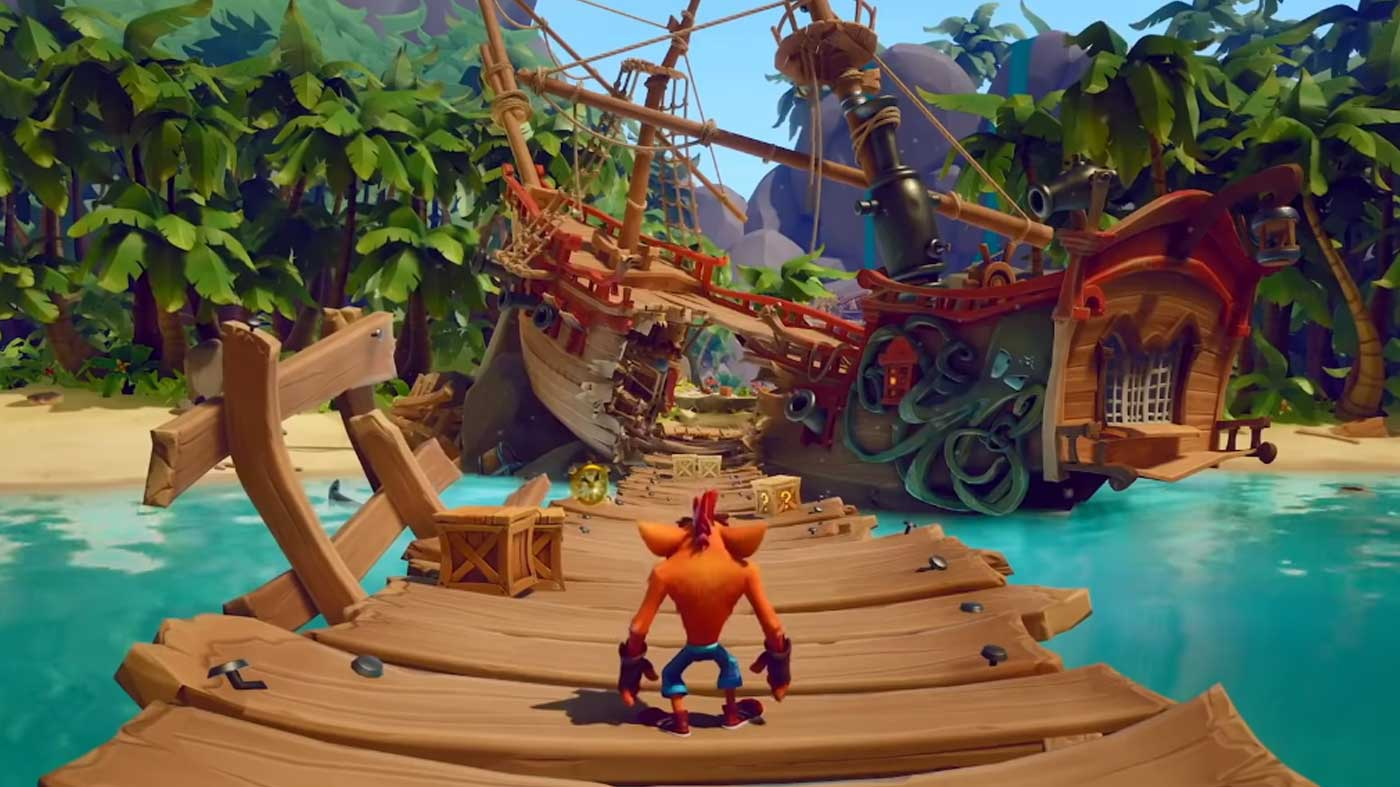
\includegraphics[width=10cm]{GamePictures/Crash.jpg}
	\caption{Crash Bandicoot 4: It’s About Time}\label{Pict:Crash}

	\centering
	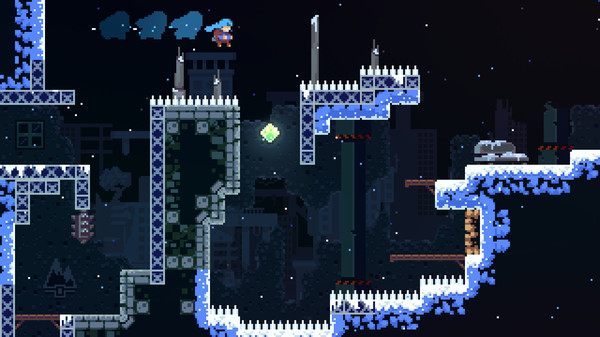
\includegraphics[width=10cm]{GamePictures/Celeste.jpg}
	\caption{Celeste}\label{Pict:Celeste}
	\centering
	\includegraphics[width=10cm]{GamePictures/Ori.jpg}
	\caption{Ori and the Blind Forest}\label{Pict:Ori}

\end{figure}

Poruszanie postaci zostanie zaprojektowane tak, aby było wymagające, ale też
intuicyjne i łatwe do zapamiętania -- obsługa klawiszy będzie podobna jak w innych
grach platformowych. Ważną częścią pisania skryptów jest optymalizacja, ze
względu na to, że w dzisiejszych czasach 60 FPS(z ang. Frames Per Second –
Klatki na sekundę) jest wymagane przez użytkowników. Dla programisty to oznacza,
że obliczenia graficzne muszą zostać wykonane w czasie 1/60 sekundy. Obliczenia
fizyczne muszą być wykonywane z taką samą częstotliwością lub szybciej od
obliczeń graficznych. Dzięki temu postać i inne poruszające się obiekty będą
poruszały się płynnie.


\clearpage

\section{Wstęp teoretyczny}

Gry są to programy, które służą głównie rozrywce. Gry komputerowe dzieli się  
na typy -- różniące się rozgrywką. Te programy można podzielić na kilka części składowych: 
\begin{enumerate}
 \item skrypty, 
 \item grafika, 
 \item udźwiękowienie, 
 \item projekt poziomu, 
 \item projekt rozgrywki.
\end{enumerate}
Waga każdego elementu zależy od gatunku gry -- przykładowo w grach strategicznych
ważną częścią są skrypty sztucznej inteligencji, z którą mierzy się gracz, a w
grach zręcznościowych ważnym elementem jest projekt poziomu. Produkcja gier jest
skomplikowanym procesem, i wymaga dużo czasu. W celu ułatwienia oraz
przyśpieszenia produkcji gier korzysta się z silników, które odpowiadają za
symulację fizyki oraz rendering elementów graficznych (wygenerowanie i
wyświetlenie obrazu gry). 
\subsection{Silnik}
\subsubsection{Najbardziej znane silniki graficzne}

Istnieje wiele silników do tworzenia gier, jednak silnikiem najprostszym i
jednym z najbardziej rozpoznawalnych jest Unity\cite{UnityPAGE} -- do skryptów używa języka
C$\sharp$. Innym silnikiem, który dominuje na rynku jest Unreal Engine\cite{UnrealPAGE} -- do
skryptów używa języka C$++$. Oba silniki posiadają swoje wady i zalety. Zaletami
Unity są prostota, skalowalność i szybkość powstawania projektów, a do wad
należy zaliczyć fakt, że rozbudowane gry często działają wolno. Zaletami Unreal
Engine są szybkość stworzonej już gry, elastyczność (silnik pozwala na bardzo
dużo i twórców ogranicza głównie wyobraźnia oraz moc obliczeniowa komputera)
oraz ilość przygotowanych elementów przez twórców, a do wad zalicza się
wymagania edytora oraz czas potrzebny na zrobienie małego projektu. Oba silniki
posiadają interfejsy graficzne do rozstawiania, przesuwania, skalowania,
obracania obiektów. Oba silniki posiadają symulator fizyki, który jest
odpowiedzialny za obliczenia związane z fizyką. Unity oraz Unreal Engine
posiadają złożone systemy oświetlenia -- obiekty, które emitują światło można
dowolnie modyfikować (położenie, kierunek, intensywność, kolor itp.)\cite{UnityVSUnreal}. 

Każdy z silników jest zbudowany w inny sposób, ale zasada działania każdego z
nich jest podobna.

\subsubsection{Kolejność działań w silniku Unity}

W silnikach graficznych, aby uniknąć nieporozumień i ułatwić pracę programistom
tworzy się tzw. Flow Chart, wykresy, które obrazują zachowanie się silnika.
Określają one kolejność wywoływania metod klasy dziedziczącej z obiektu
bazowego. W Unity obiektem bazowym każdej klasy skryptu w obiektach jest
MonoBehaviour. Na rysunku\ref{Fig:UnityFlowChart} znajduje się podział kolejność
wywoływania metod -- zaczynając od góry. 
\begin{figure}[hb!]
	\centering
	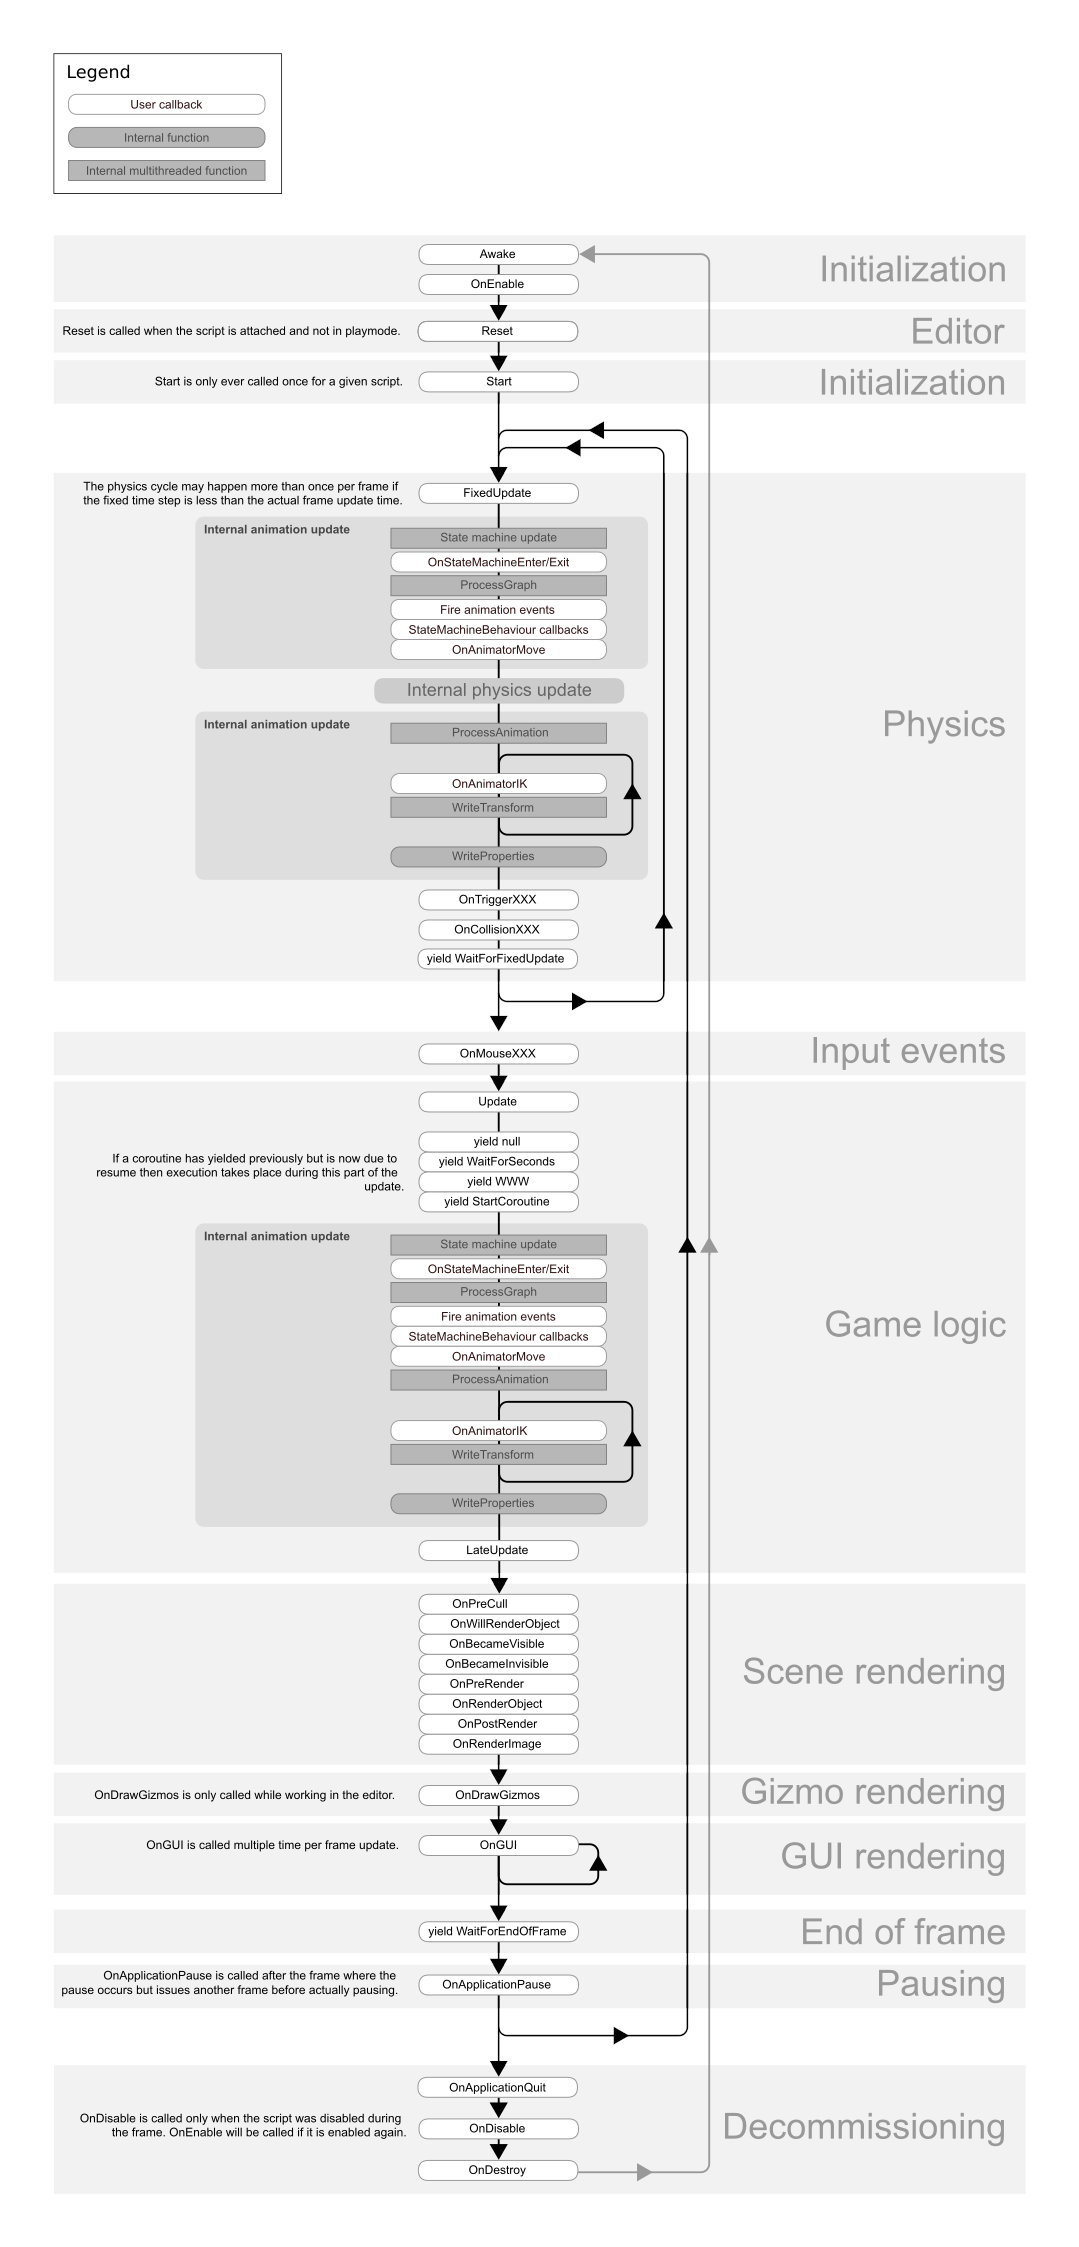
\includegraphics[width=10cm]{Charts/monobehaviour_flowchart.jpg}
	\caption{Unity flowchart}
    \label{Fig:UnityFlowChart}
\end{figure}
Każdy blok odpowiada metodzie w klasie bazowej MonoBehvior, z której dziedziczy
każda klasa przypięta do obiektu w silniku Unity. Każdą z tych metod można
nadpisać. Każdy obiekt ma pewien czas życia -- czas, w którym obiekt jest obecny
w grze. Bloki białe -- metody, które można nadpisać Broki szare -- skrypty silnika
Unity, tych metod nie można nadpisać Podczas życia obiektu zachodzi wiele
obliczeń, które można podzielić na kilka etapów. W każdym etapie znajdują się
metody do wpływania na program. Metody inicjalizacji obietku\cite{UnityFlow}:
\begin{itemize}

\item void Awake() -- metoda wywoływana, gdy obiekt GameObject został
zainicjalizowany, gdy scena zawierająca obiekt została załadowana, obiekt
wcześniej nieaktywny został aktywowany lub obiekt został stworzony używając
metody Object.Instantiate. Metoda jest wywoływana tylko raz w trakcie życia
instancji skryptu 
\item void OnEnable() -- metoda zostaje wywoływana, gdy skrypt jest aktywowany –
wywołanie metody -- SetActive(true), gdy skrypt poprzednio był nieaktywny. 
\end{itemize}
Pętla Fizyczna -- obliczenia związane z fizyką, mogą być wywoływane kilkukrotnie
w ciągu klatki:
\begin{itemize}
\item void FixedUpdate() -- metoda pętli fizycznej, może być wywoływana więcej
razy niż metoda Update. W tej metodzie powinny się znaleźć metody, które
odpowiadają za fizykę gry (nie muszą się tutaj znajdować).
\item void OnStateMachineExit/Enter(Animator animator, int stateMachinePathHash)
– za argumenty przyjmują component animatora oraz numer maszyny stanu w
animatorze. Metody działają na tej podobnej zasadzie -- jedna jest wywoływana na
zakończenie animacji, a druga podczas włączenia następnej animacji
\item void FireAnimationEvent(void/float/string/int/object) -- metoda wywoływana
w pewnym miejscu animacji, oznaczonym w edytorze animacji silnika Unity –
zakładka `Animation' w inspektorze silnika. 
\item StateMachineBehaviour callbacks -- wywoływanie metod klasy
StateMachineBehaviur. Klasa ta jest używana do skryptów używanych w trakcie
działania pewnych animacji. 
\item void OnAnimatorIK(int) -- wywoływana przed aktualizacją wewnętrznego
systemu IK (inverse kinematics).
\item metody OnTriggerXXX i  OnCollisionXXX -- metody wywoływane podczas detekcji
kolizji -- są 3 rodzaje metod Enter (kolizja się rozpoczęła), Stay (kolizja trwa)
i Exit (zakończenie kolizji). Są 2 typy kolizji w silniku Unity, kolizje typu
collider-collider i typu collider-trigger. Kolizje collider-collider będą
wywoływać metody OnCollisionXXX oraz powodują że obiekty nie  `wchodzą' w
siebie. Kolizje typu collider-trigger wywołują metody typu OnTriggerXXX oraz
powodują że jeden obiekt przechodzi przez drugi (collider typu trigger jest
traktowany jak powietrze w kolizjach). Kolizje typu trigger-trigger nie
występują.
\item yield return -- sygnalizuje, że dalsza część programu zostanie wykonana
później. Nie jest to metoda, a korutyna (Coroutine). 
\item yield return WaitForFixeUpdate -- kontynuacja wykonywania metod po metodzie
FixedUpdate
\end{itemize}
Input Events (zdarzenia wejścia) -- w tym miejscu wywoływane są zdarzenia
urządzeń wejścia. Graf może się różnić, gdy jest używana paczka `Input system',
która obsługuje te zdarzenia. Logika Gry (Game Logic):
\begin{itemize}
\item void Update() -- metoda wywoływana raz na klatkę. Powinna zawierać skrypty do zarządzania GUI, animacjami oraz elementy logiki gry.
\item yield return null -- kontynuacja skryptu w następnej klatce
\item yield return WaitForSeconds -- kontynuacja skryptu po  podanej liczbie sekund
\item yield return WWW -- kontynuacja skryptu po ściągnięciu obiektu z strony www
\item yield return StartCoroutine -- kontynuacja skryptu po zakończeniu metody
\item void LateUpdate() -- wywoływana pod koniec logiki gry. Najczęściej używana do ustawiania kamery.
\end{itemize}
Scene rendering:
\begin{itemize}
    \item void OnPreCull() -- metoda wywoływana przed obcięciem sceny do pola
    widzenia kamery.
    \item void OnWillRenderObject() -- metoda wywoływana dla każdej kamery jeżeli
    obiekt jest widoczny (a nie jest elementem UI).
    \item void OnBecameVisible() -- metoda wywoływana, gdy obiekt jest widoczny
    przez jakąkolwiek kamerę.
    \item void OnBecameInvisible() -- metoda wywoływana, gdy obiekt nie jest
    widoczny w żadnej z kamer. 
    \item void OnPreRender() -- metoda jest wywoływana przed renderowaniem sceny.
    \item void OnRenderObject() -- metoda jest wywoływana w trakcie renderowania
    sceny.
    \item void OnPostRender() -- metoda jest wywoływana po wyrenderowaniu sceny.
    \item void OnRenderImage(RenderTexture,RenderTexture) -- pozwala na
    modyfikacje końcowego obrazu kamery. Najczęściej używana do efektów tzw.
    post procesing`u.
\end{itemize}
Gizmo rendering -- jest to renderowanie elementów do debugowania. Metoda void
OnDrawGizmos() pozwala na nałożenie tych elementów. Będą one nałożone na resztę
obiektów. GUI rendering -- render elementów graficznego interfejsu użytkownika.
Posiada tylko metodę  
void OnGUI().  Rekomendowane jest używanie tej metody do modyfikacji elementów
UI i obsługę zdarzeń tych elementów (np. przycisków). Jest wywoływana
wielokrotnie w ciągu klatki. Etap End Of frame kontynuuje program w miejscu
wywołania yield return WaitForEndOfFrame. Decommisioning -- etap w którym kończy
się życie obiektu. Metody void OnApplicationQuit() -- wywoływana podczas wyjścia
z programu --  void OnDissable() -- zablokowanie wykonywania skryptu, wywoływana w
klatce, w której został on zablokowany -- void OnDestroy() -- metoda do
zniszczenia obiektu, w tym miejscu powinny zostać zwolnione zasoby.

\subsection{Grafika}

W dzisiejszych czasach do modelowania oraz tworzenia animacji używa się
wyspecjalizowanych do tego programów. Najczęściej używanym programem jest
Blender\cite{blender_URL} -- darmowy program związany z trójwymiarową grafiką komputerową. Jest
programem najczęściej wybieranym ze względu na zaawansowanie oraz fakt, że
wszystkie narzędzia są w jednym programie. Jest to bardzo pomocne podczas
tworzenia modeli i animacji.  
Tekstury są to różne mapy, które nakładane są na model --  najczęściej używane to
mapy kolorów, normalnych i oświetlenia (ambient, diffuse, specular). Tekstury
można generować proceduralnie lub tworzyć ręcznie za pomocą programów
graficznych. Tekstury generowane graficznie tworzone są szybciej jednak wymagają
wypalania -- proces, który zapisuje teksturę wygenerowaną do pliku --  co wymaga
dużo czasu. Największą zaletą generacji tekstur jest efekt nakładania się map,
dzięki któremu mapy wyglądają naturalnie (najczęściej rozjeżdżają się mapy
normalnych i oświetlenia).  Do tworzenia tekstur można użyć programów do tego
dedykowanych (np. Quixel Mixer), które wspierają np. warstwy.
\subsection{Projekt poziomów}

Poziomy tworzone są proceduralnie lub ręcznie. Proceduralna generacja poziomów
dotyczy tylko określonych gier lub terenu. Pełna generacja poziomów zwykle
dotyczy określonych gatunków gier, gdzie twórcy zakładają przechodzenie gry
wielokrotnie np. Deadcells (\ref{Pict:Dead Cells}) lub bardzo ważnyme elementem
jest proceduralna generacja poziomów np. Minecraft (\ref{Pict:Minecraft}),
Terraria (\ref{Pict:Terraria}). Tworzenie ręczne poziomów często wykorzystuje
generację terenu (najczęściej obejmuje góry, jaskinie, polany). W innym wypadku
pozostaje ręczne tworzenie terenu -- ten proces jest bardzo czasochłonny. Na
przygotowaną mapę terenów nakładane są modele drzew, krzewów, budynków itp.
Narzędzia do tworzenia poziomów (generowanych i tworzonych ręcznie) są dostępne
w silnikach lub zostały przygotowane dodatki lub wtyczki do tego celu.
\begin{figure}[ht!]
	\centering
	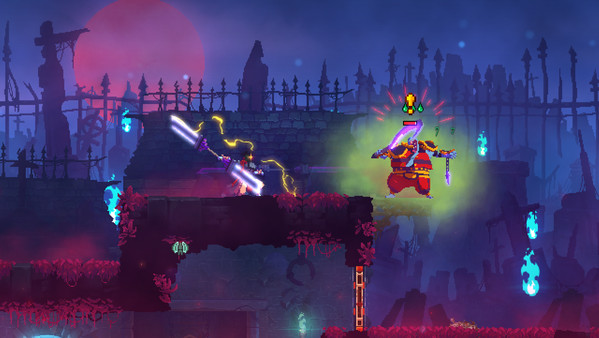
\includegraphics[width=10cm]{GamePictures/DeadCells.jpg}
	\caption{Dead Cells}
    \label{Pict:Dead Cells}
\end{figure}



\begin{figure}[ht!]
	\centering
	\includegraphics[width=10cm]{GamePictures/Minecraft.jpg}
	\caption{Minecraft}
    \label{Pict:Minecraft}
\end{figure}



\begin{figure}[ht!]
	\centering
	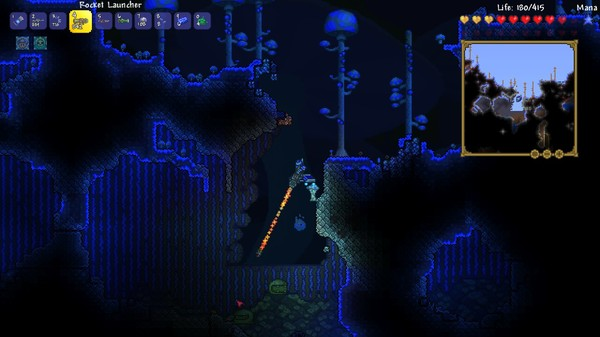
\includegraphics[width=10cm]{GamePictures/terraria.jpg}
	\caption{Terraria}
    \label{Pict:Terraria}

\end{figure}



\clearpage	



\section{Wprowadzenie do programu Blender}
\subsection{Blender -- pola robocze i tryby}
Blender jest programem, który jest bardzo elastyczny. To stwierdzenie dotyczy
też modyfikacji przestrzeni roboczej. Domyślnie w wersji programu v3.3 posiada
11 układów stworzonych przez twórców –- Layout, Modeling, Sculpting, UV Editing,
Texture  Paint, Shading, Animation, Rendering, Compositing, Geometry Nodes,
Scripting (pole nr. 1 na rysunku \ref{Bledner:workspaces})-- każdy z nich jest
stosowany do innych celów. Możliwe jest też tworzenie własnych układów co zostało
opisane w dokumentacji programu \cite{blender_window_workspaces}. 
Znajdują się one w pasku u góry okna programu (na rysunku
\ref{Bledner:workspaces} nr. 1).Na rysunku pola 2, 3, 4 i 5 są obszarami
roboczymi, które można zmieniać. \cite{blender_workspace_show} Rysunek
\ref{Bledner:workspaces} nr.2 domyślnie przedstawia widok na scenę. Zawartość
każdego pola roboczego można zmienić klikając w ikonę w lewym górnym rogu pola
roboczego -- zawarte są tutaj różnego rodzaju pola robocze do np. edytowania
shader`ów, podglądu sceny czy edytory animacji. Obok znajduje się tryb danego
pola roboczego -- w nie każdym polu roboczym taki się znajduje, ponieważ niektóre
pola robocze nie mają innych trybów -- który pozwala na jego zmianę. Domyślną
zawartością pola nr. 3 –- `Outliner' -- jest lista obiektów znajdujących się na
scenie. Obiekty można grupować w kolekcje. W niektórych przypadkach obiekty mogą
zawierać w sobie inne obiekty. Obszar nr. 4 standardowo jest obszarem kontroli
czasu -- nazywa się `Timeline' -- używanym głównie przy tworzeniu animacji. W
obszarze nr. 5, który nazywa się `Properties' domyślnie znajdują się właściwości
obiektu, sceny itp. 

\begin{figure}[h!]
    \centering
    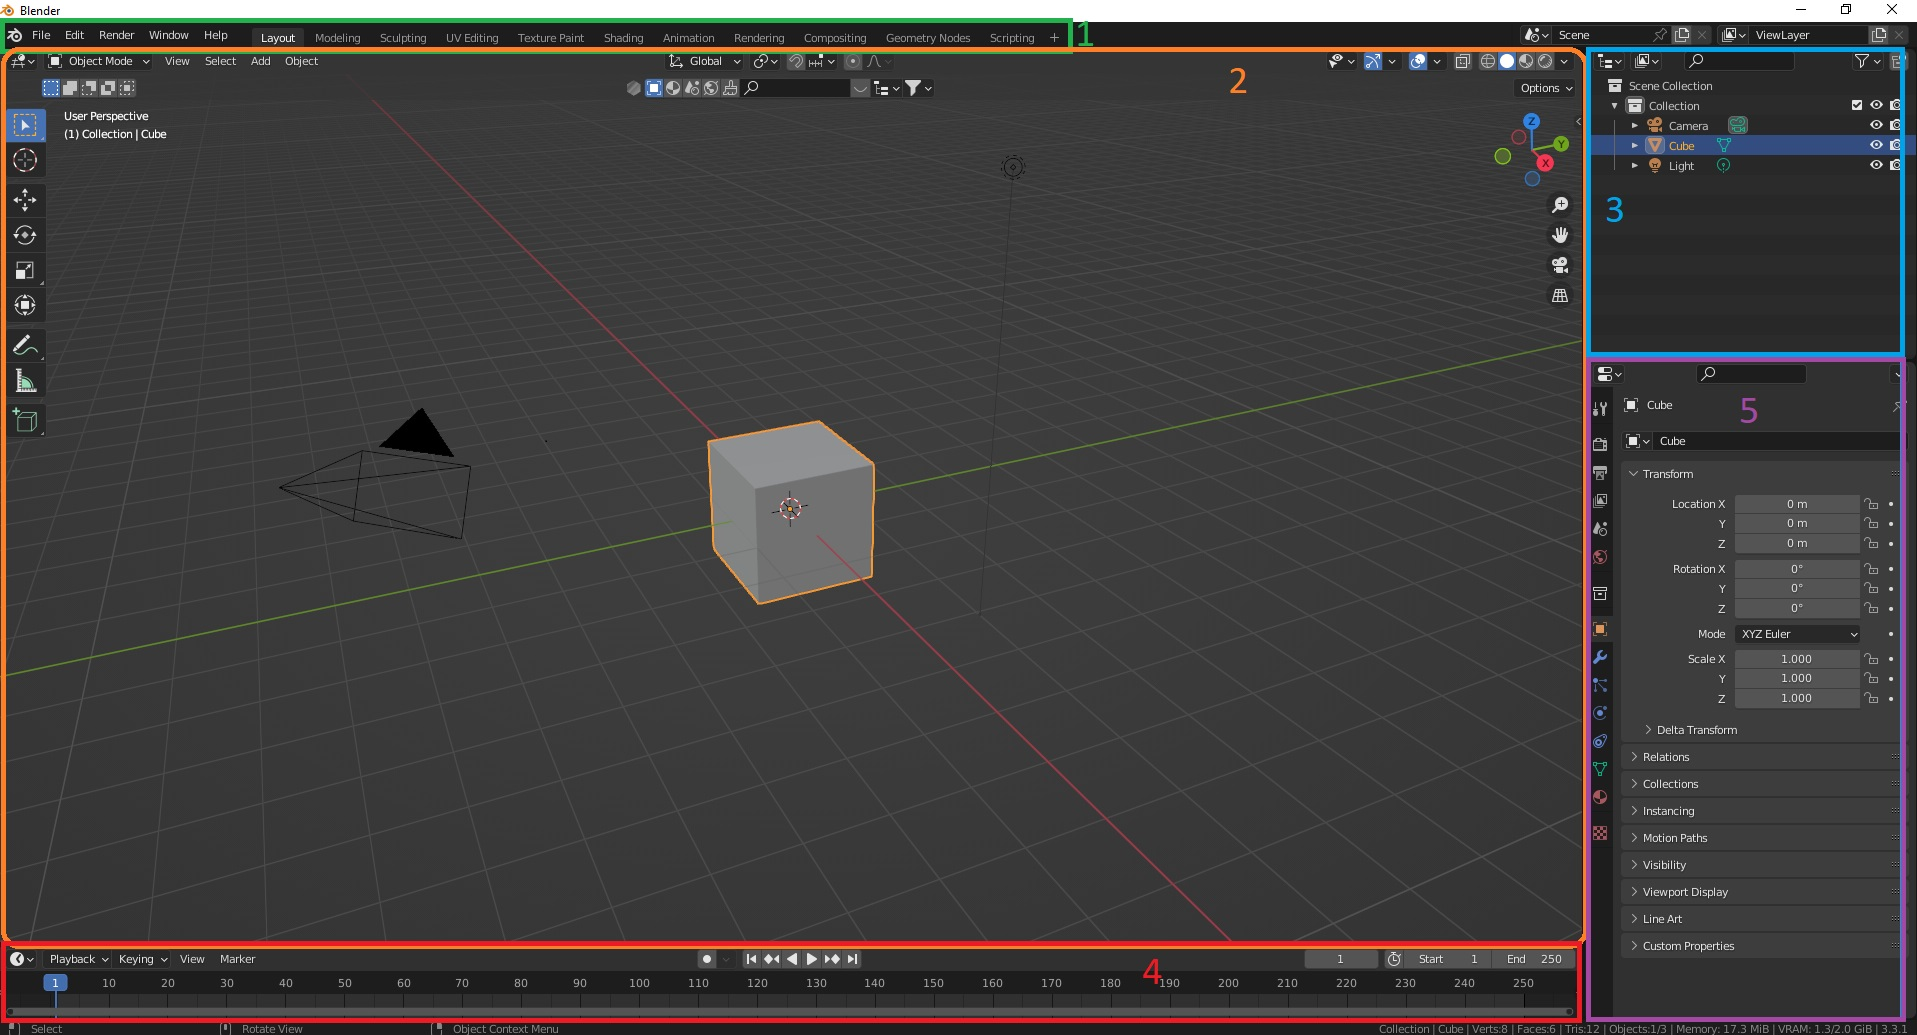
\includegraphics[width=16cm]{BlenderPict/default_window_segments.jpg}
    \caption{Blender podział przestrzeni roboczej}
    \label{Bledner:workspaces}
\end{figure}

Niektóre tryby są dostępne po zaznaczeniu odpowiedniego obiektu -- np.
`Pose mode', za pomocą którego tworzy się animacje jest dostępny tylko w wypadku
zaznaczenia obiektu typu `Armature'. Do zrobienia modeli najczęściej używa się
trybów `Edit mode' i `Sculpt mode'. Pierwszy z nich pozwala na tworzenie
prostych siatek za pomocą narzędzi do skalowania, rotacji, przesuwania i
tworzenia nowych ścian, krawędzi i/lub wierzchołków. `Sculpt mode' jest trybem,
który można porównać do tworzenia glinianej rzeźby -- narzędzia pozwalają na
wycinanie, spłaszczanie płaszczyzn, rozciąganie itp. Posiada nawet pędzel
symulujący tkaniny. Tworzenie modeli wymaga sporo czasu i doświadczenia w
używaniu tych dwóch trybów.

\subsection{Kości i szkielety -- podstawy animacji szkieletowych}
Szkielet -- w programie Blender obiekt szkieletu nazywa się `Armature' -- jest
zbiorem kości, które są ze sobą w połączone w relacji rodzic -- dziecko. Relacja
ta polega na tym, że kość rodzica wpływa na dzieci. Każda kość może, ale nie musi
mieć rodzica -- tak samo jest w przypadku dzieci. Kości mają początek -- nazwany
`Head' -- i koniec -- nazwany `Tail'. Na kości mogą działać modyfikatory –
specjalne operacje z dziedziny animacji, które ułatwiają animowanie. Kości
jedynie wpływają na siatkę -- obiekt typu `Mesh' -- deformując ją. Kości nie są
wyświetlane i służą tylko do deformacji. Jest to możliwe poprzez nakładanie wagi
– współczynnika -- z jaką dana kość wpływa na dany punkt w siatce. Edytowanie wag
jest możliwe  w trybie `Weight Paint' -- należy zaznaczyć wybrać obiekty
`Armature' i `Mesh'. '. Jeden obiekt typu `Armature' może deformować wiele
obiektów typu `Mesh'.


Do stworzenia szkieletu używa się `Edit mode', gdy zaznaczony jest obiekt typu
`Armature'. W tym trybie można tworzyć nowe kości, zmieniać ich rozmiar, relacje
- określanie czyje i jakie transformacje ma dziedziczyć –- czy określać, czy dana
kość deformuje siatkę. Trybem używanym do robienia animacji jest wcześniej
wspomniany tryb `Pose mode'. W tym trybie wcześniej stworzony szkielet działa
według określonych zasad:
\begin{itemize}
\item jeżeli kość ma rodzica i jest `connected' to wtedy nie może się od tego
rodzica odczepić -- początek kości będzie pyrzczepiony dokońca kości rodzica
\item jeżeli kość ma odznaczoną opcję `inherit Rotation' to rotacja rodzica nie
rotuje tej kości, ale ją przesuwa
\item modyfikatory mogą działać niezależnie od zaznaczenia pól `connected' i
`inherit roation'
\end{itemize}
Położenie pól `connected' i `inherit Rotation' pokazano na rysunku
\ref{Blender:ConnectedInherit} znajduje się ono w polu roboczym `Properties',
zakładka `Relations' w zakładce `Bone Properties', tutaj znajduje się
również informacja, która kość jest rodzicem i opcja do zmiany czy dana kość
deformuje siatkę -- pole `Deform'. Zakładka `Bone Properties' jest dostępna po wybraniu
obiektu typu `Aramature' -- w trybie `Object Mode' też jest dostępna, ale nie
działa poprawnie, a poprawne działanie jest w trybach `Edit Mode' i `Pose Mode'.

\begin{figure}[ht]
    \centering
    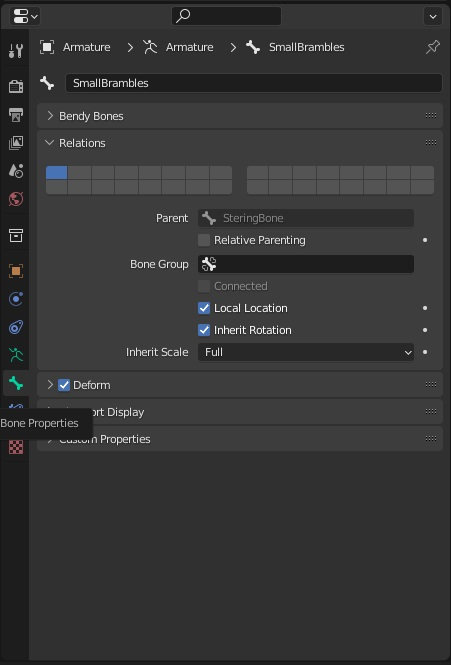
\includegraphics[width=7cm]{BlenderPict/Bone_Properties.jpg}
    \caption{Miejsze zmiany własciwości Kości}
    \label{Blender:ConnectedInherit}
\end{figure}

Rysunek \ref{Blender:Constraints} pokazuje położenie zakładki zawierającej
modyfikatory kości -– zakładka nazywa się `Bone Constraints Properties' i jest
dostępna tylko w trybie `Pose mode'. Narzędzia tutaj zawarte bardzo ułatwiają
tworzenie animacji szkieletowych --  jest ich 28 w 4 różnych kategoriach
pokazanych na rysunku \ref{Blender:Constraints_List}. 

\begin{figure}[hb!]
    
    \centering
    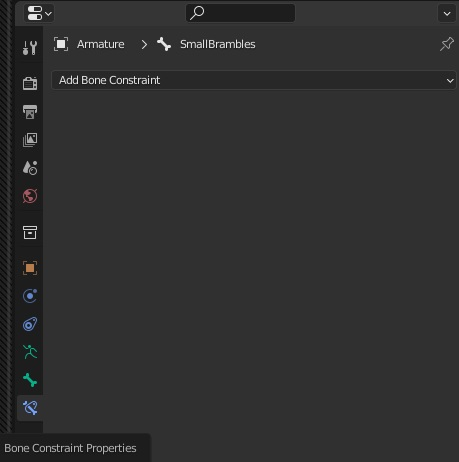
\includegraphics[width=12cm]{BlenderPict/Bone_Constraints.jpg}
    \caption{Miejsce zmiany własciwości Kości}
    \label{Blender:Constraints}
\end{figure}

\begin{figure}[hb!]
    \centering
    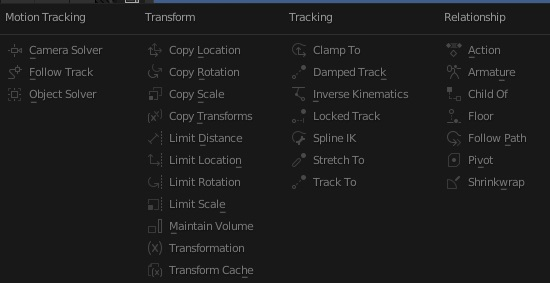
\includegraphics[width=12cm]{BlenderPict/Bone_Constraints_list.jpg}
    \caption{Lista modyfikatorów dostępnych w programie}
    \label{Blender:Constraints_List}
\end{figure}

W projekcie zostały użyte następujące modyfikatory kości:
\begin{itemize}
\item Inverse Kinematics 
\item Copy Location  
\item Copy Transforms
\end{itemize}
\subsubsection{Modyfikator Inverse Kinematics}
Modyfikator Inverse Kinematics (rysunek \ref{Blender:IK}) wpływa na kość
posiadającą ten modyfikator oraz rodziców -- w zależne ile zostało ustawione w
parametrze `Chain Length'. Efektem jest umieszczenie końca kości w pewnej
pozycji -- początku innej kości. Kości, na które wpływa modyfikator są nazywane
łańcuchem. Za parametry przyjmuje:
\begin{itemize}
\item Target -- jest to obiekt, który będzie brany jako punkt, w którym koniec kości ma się znaleźć. W przypadku wybrania obiektu typu `Armature' należy wybrać również kość tego obiektu.
\item Bone -- jest to kość w obiekcie `Armature'. 
\item Pole Target -- obiekt, który określa, w którym kierunku ma zostać wygięty dany łańcuch. Można powiedzieć, że ten obiekt odpowiada za rotację łańcucha w odpowiednim kierunku.
\item Pole Angle -- stosowane do korygowania wygięcia łańcucha
\item Iterations -- określa ile maksymalnie iteracji obliczeń ma się odbyć w celu obliczenia transformacji kości
\item UseTail -- pole określa czy początek kości może być ostatnim elementem łańcucha
\item Stretch -- pozwala/zabrania na rozciąganie kości
\item Rotation -- stopień w jakim brana jest pod uwagę rotacja obiektu `Target'
\item Influence -- stopień wpływu modyfikatora na kości w łańcuchu
\end{itemize}
\begin{figure}[ht!]
    \centering
    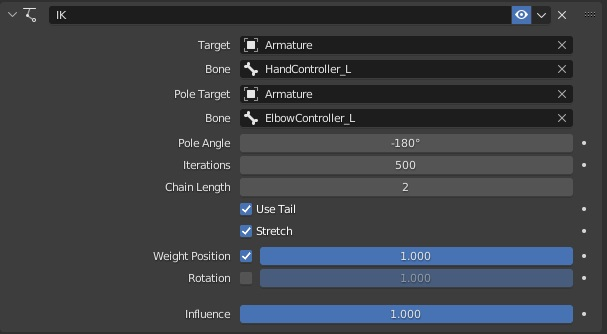
\includegraphics[width=12cm]{BlenderPict/Constraints_IK.jpg}
    \caption{Modyfikator kości Inverse Kinematics}
    \label{Blender:IK}
\end{figure}

Ten modyfikator przydaje się podczas animacji kości, które poruszają się w
jednej płaszczyźnie lub każda z kości może rotować się w jednej płaszczyźnie –
np. noga, ręka lub palce. Przy bardziej skomplikowanych odcinkach -- np.
kręgosłup -- modyfikator IK nie sprawdza się. 

\subsubsection{Modyfikator Copy Location i Copy Transforms}
Copy Location (rysunek \ref{Blender:CopyLocation}) jest modyfikatorem odpowiadającym za m.in. skopiowanie pozycji
innej kości w określonym układzie odniesienia -- wpływa na kość posiadającą
ten modyfikator.

Modyfukator posiada następujące pola (rysunek \ref{Blender:CopyLocation}):
\begin{itemize}
    \item Target -- obiekt, od którego kopiowana jest położenie. W przypadku wybrania obiektu typu `Armature' pojawia się pole `Bone' -- kość wybranego szkieletu
    \item Head/Tail -- określa czy kopiowana ma być kopiowana od początku czy końca wybranej kości
    \item Axis -- określa czy wszystkie współrzędne mają być kopionwane.
    \item Invert -- pozwala wybrać, które współrzędne mają by odwrócone -- jeżeli zaznaczone wtedy dana współrzędna jest mnożona przez -1
    \item Offset -- jeżeli opcja będzie zaznaczona to kopiowane współrzędne będą traktowane jako przesunięcie.
    \item target -- jest to układ odniesienia, z którego kopiowane będą wpółrzędne. Dostępne są następujące układy odniesienia \cite{blender_Space_Types}:
    \begin{itemize}
	\item World Space (przestrzeń globalna) -- punktem odniesienia jest punkt (0,0,0).
	\item Local Space (przestrzeń lokalna) -- brane są transformacje względem obiektu rodzica.
	\item Local with Parent (lokalna z rodzicem) tylko dla kości. Transformacje są oceniane względem położenia i orientacji w pozie spoczynkowej.
	\item Pose Space (przestrzeń pozy) tylko dla kości. Działa podobnie do globalnego układu odniesienia tyle że punktem odniesienia jest transformacja głównego obiektu `Armature'.
	\item Custom Space (przestrzeń niestandardowa) -- transformacje są oceniane względem bieżącej pozycji i orientacji wybranego obiektu.
	\item Local Space (Owner Orientation)  tylko dla kości `Target'.  Ta przestrzeń pozwala na taki sam ruch kości która kopiuje transformacje pod warunkiem, że kości rodzice są w pozie spoczynkowej.
    \end{itemize} 
    \item Owner pole podobnie jak target określna do jakiej przestrzeni będą kopiowane współrzędne przemieszczenia. 
\end{itemize}


\begin{figure}[ht]
    \centering
    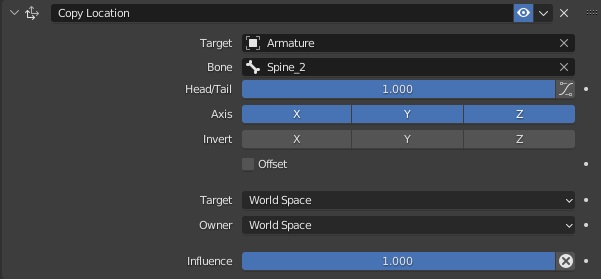
\includegraphics[width=12cm]{BlenderPict/Constraints_Copy_Location.jpg}
    \caption{Modyfikator kości Copy Location}
    \label{Blender:CopyLocation}
\end{figure}

Modyfikator Copy Transforms jest rozwinięciem modyfikatora Copy Location -- poza kopiowaniem lokacji kopiuje jeszcze skalę i rotację. Na rysunku \ref{Blender:CopyTransform} widać, że ten modyfikator jest obcięty z możliwości wybrania kopiowanych osi. Zamiast tego posiada pole `Mix', w którym można określić w jaki sposób w jaki sposób transformacje kopiowane ingerują w transformacje kości-właściciela. W tym polu można ustawić następujące wartości:
\begin{itemize}
	\item Replace -- podmienia transformacje na transformacje obiektu w polu `Target' lub wybranej kości.
	\item Before/After Original (Full) -- Nowa transformacja jest dodawana przed (Before) lub po (After) macierzy właściciela. Full oznacza, że skala jest w pełni dziedziczona -- jest wyliczona z wszystkich rodziców obiektu, z której kopiowane są transformacje.
	\item Before/After Original (Aligned)  -- Nowa transformacja jest dodawana przed (Before) lub po (After) macierzy właściciela. Aligned oznacza, że kość jest skalowana o całkowitą skalę obiektu `Target' lub wybranej kości.
	\item Before/After Original (Split Channels) -- w tym trybie rotacja, skala i lokacja są rozdzielane na osobne kanały. W tym przypadku kanały lokacji są dodawana oddzielnie od kanałów rotacji i skali, dzięki czemu skala i rotacja nie mają wpływu na lokacje.
\end{itemize} 

\begin{figure}[ht]
    \centering
    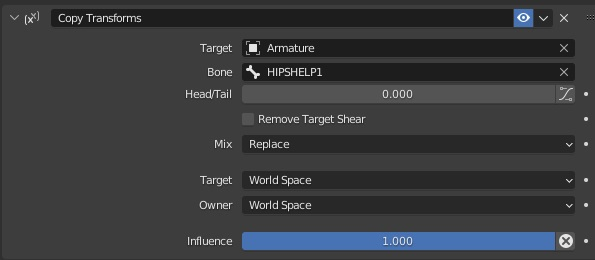
\includegraphics[width=12cm]{BlenderPict/Constraints_Copy_Transforms.jpg}
    \caption{Modyfikator kości Copy Transforms}
    \label{Blender:CopyTransform}
\end{figure}
\clearpage
\subsection{Weight Paint -- deformacja siatki przez szkielet}
`Weight Painting' jest procesem polegającym na przypisaniu wagi kości
wierzchołkom. W ten sposób siatka zmienia się odpowiednio według zmian
transformacji kości. W celu zainicjalizowania ‘połączenia’ siatki  i szkieletem
należy wybrać obiekt siatki –`mesh`- i obiekt szkieletu -- `Armature` -- jak na
rysunku \ref{Blender:ArmatureDeform} i następnie wcisnąć klawisze ‘CTRL’ i ‘P’ w tym samym czasie, co
otworzy menu jak na rysknku, a opcjami odpowiedzialnymi za związanie ze sobą
tych obiektów są 3 poniżej opcji ‘Armature Deform’. Wynikiem `With Empty Groups`
sprawi, że każda kość nie będzie miała wag. `With Automatic Weights` sprawi, że
wagi będą tworzone automatycznie na podstawie odległości -- wagi często są
błędnie wyliczane. Ostatnia opcja `With Envelope Weights` wykorzystuje ‘Bone
Envelope’ -- strefę wpływów kości. Problemem tej metody jest problematyczne
ustawianie ‘Stref wpływów’. 

\begin{figure}[h]
    \centering
    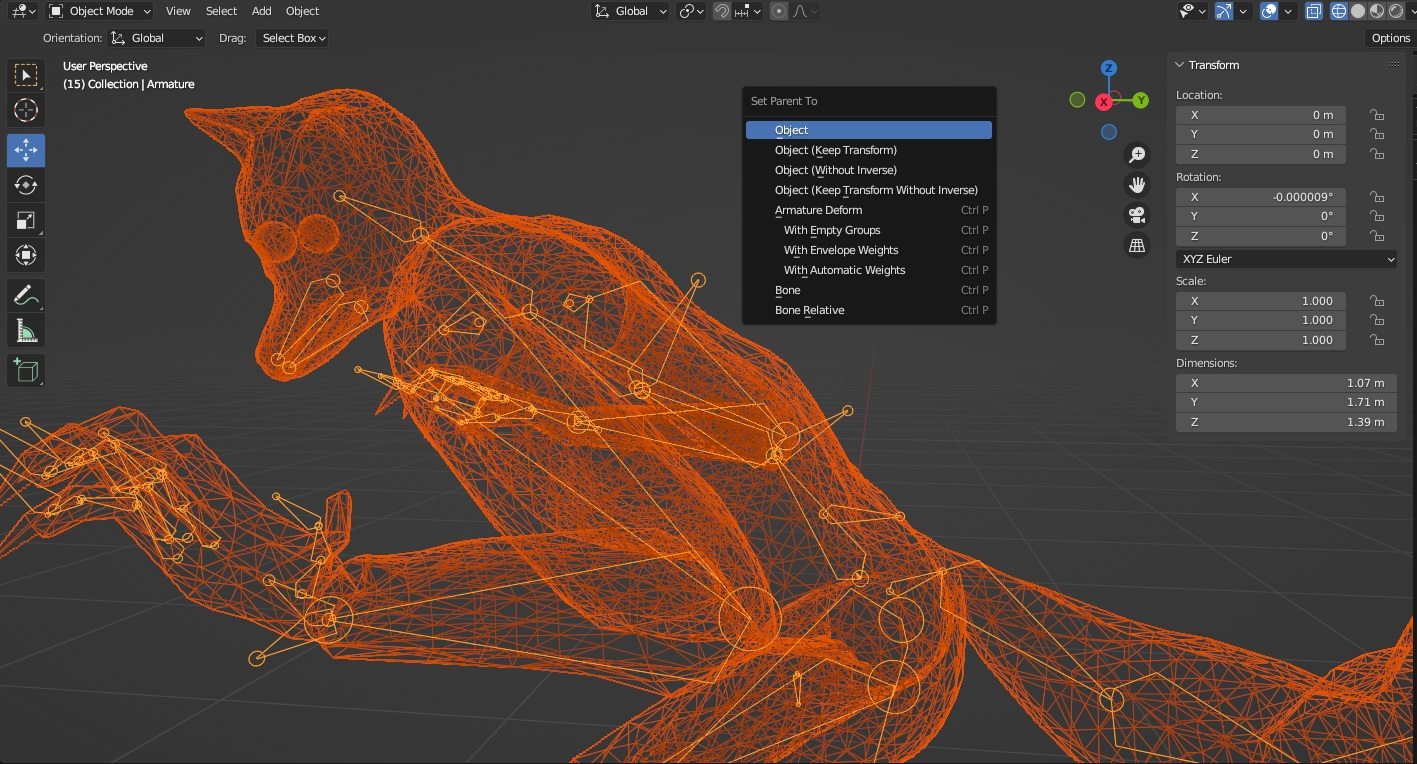
\includegraphics[width=12cm]{BlenderPict/WeightPaint_ArmatureDeform.jpg}
    \caption{Wstępne wyliczenie wag kości }
    \label{Blender:ArmatureDeform}
\end{figure}

Szkielet może deformować wiele siatek w tym samym czasie. Dlatego w programie
Blender wybór siatek odbywa się w trybie obiektowym. Na rysunku
\ref{Blender:BeginWeightPaint} znajduje się przykładowy wybór siatki do `Weigt
Painting’u'. 
\begin{figure}[h]
    \centering
    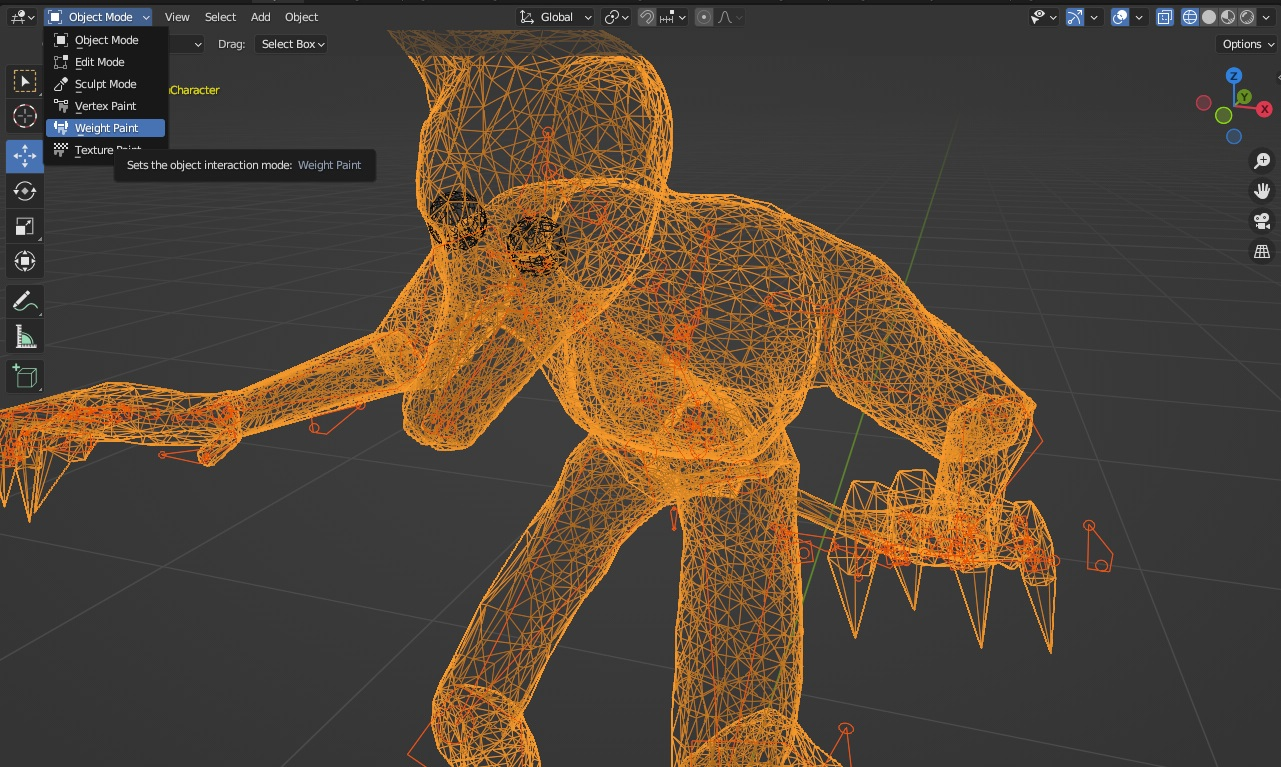
\includegraphics[width=12cm]{BlenderPict/WeightPaint_BeginWeightPaint.jpg}
    \caption{Wstępne wyliczenie wag kości }
    \label{Blender:BeginWeightPaint}
\end{figure}

Poziom wpływu danej kości na obszarze jest wyrażony w postaci kolorów. Kolor
niebieski reprezentuje brak wpływu kości na siatkę na danym obszarze, kolorem
czerwonym oznaczono wagę 1 dla danej kośći, a kolorem różowym oznaczono kości, które nie mają
stworzonej mapy do deformacji. Na rysunku \ref{Blender:SampleWeightPaint} pokazano jak wygląda mapa wag
dla kości. Kości można zmieniać poprzez kliknięcie lewym przyciskiem myszy kość
z wciśniętym klawiszem `CTRL'. Do malowania wag są dostępne różne pędzle.
Zostały one opisane bardzo dobrze w filmie \cite{blender_WeightPaint_brushes} –
narzędzia pokazane są na starszej wersji programu, ale sam film jest nadal
aktualny.

\begin{figure}[h]
    \centering
    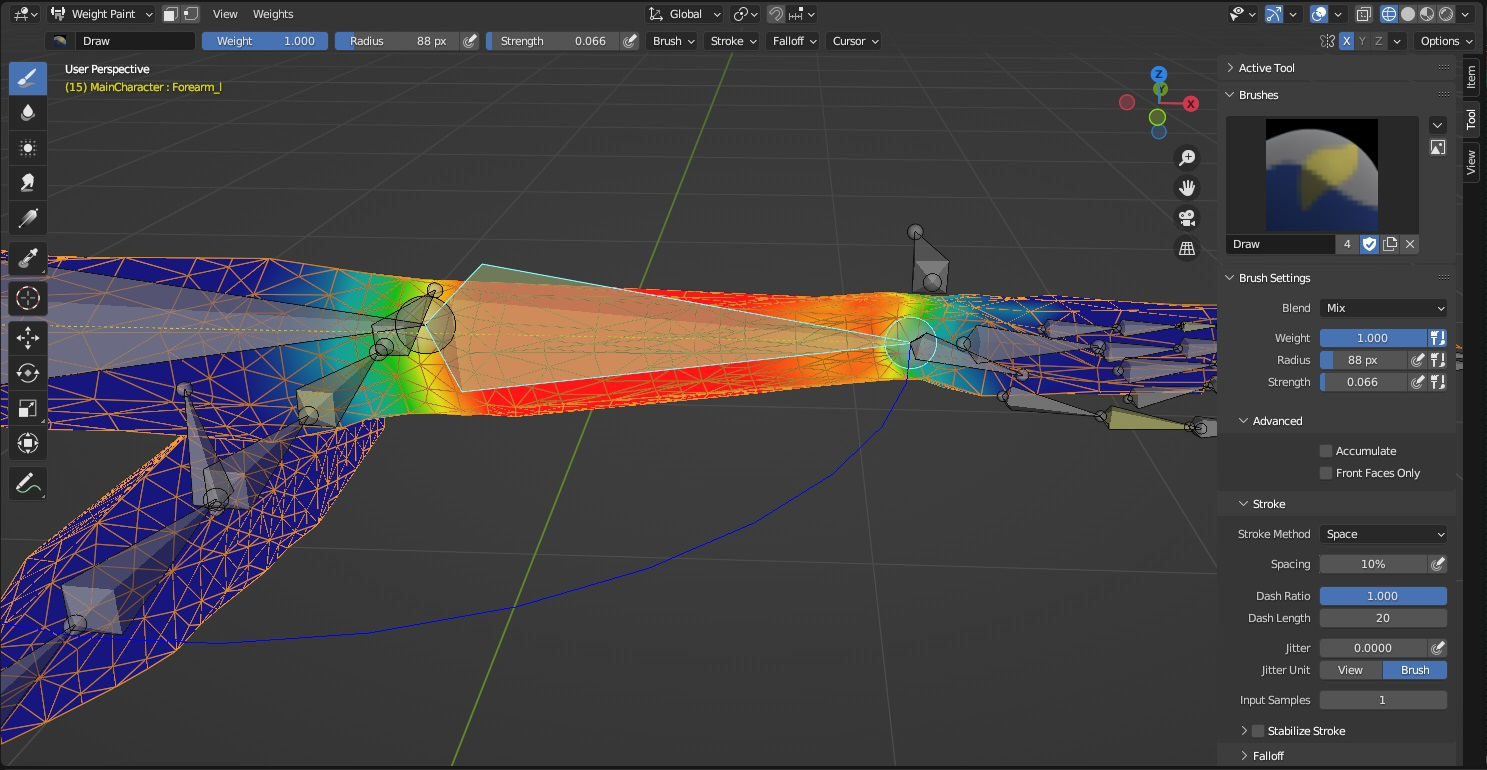
\includegraphics[width=12cm]{BlenderPict/WeightPaint_weights.jpg}
    \caption{Wstępne wyliczenie wag kości dla kości przedramienia}
    \label{Blender:SampleWeightPaint}
\end{figure}



\clearpage
\subsection{Kluczowanie klatek -- animowanie w programie Blender}
Animacja jest to -- ogólnie mówiąc -- ruch pewnego obiektu na obrazie. W grafice
2D zwykle odbywa się poprzez zmianę obrazów. W grafice 3D jest to bardziej
skomplikowane, ponieważ polega na zmianie stanu obiektu w czasie.  W grach komputerowych animacje nie
wymagają takiej jakości jak w przypadku filmów. Jakość animacji w danym
segmencie gry często jest zależna od dynamiki segmentu -- jeżeli gra jest szybka,
gracz nie będzie zwracał dużej uwagi na animacje. Tworzenie animacji jest
również czasochłonne, a im bardziej dokładna animacja tym bardziej czasochłonne
są nanoszone ewentualne poprawki. Dlatego do tworzenia animacji używa się
technologii `Motion Capture' -- technologia pozwalająca na przechwytywanie ruchu
aktorów. Problemem tego rozwiązania jest jego koszt –
sprzęt jest drogi, a dane trzeba przetworzyć co też wymaga czasu. Kontrą do tego
rozwiązania jest własnoręczne tworzenie animacji w programach graficznych. 

Ręczne tworzenie animacji wymaga kluczowania klatek. Jest to proces, w którym
zapisuje się transformacje i inne właściwości. W tym celu Blender udostępnia wiele narzędzi
pozwalających na animowanie. Na rysunku
\ref{Blender:DefaulAnimationWin} przedstawiono zestaw pól roboczych używanych do
animacji. Składają się na nie: 
\begin{itemize}
\item Pierwszym polem roboczym -- najbardziej po lewej --  jest `3D Viewport'. 
\item Na środku znajduje `Action Editor' z pola roboczego `Dope Sheet'.
\item Po lewej stronie okna znajdują się właściwości i zawartość sceny.
\item Na dole jest 'Timeline '
\end{itemize}
Taki zestaw pozwala na stworzenie zestawu animacji bez potrzeby przełączania się
między polami roboczymi. Animacje zostają zapisane w jako tzw. Akcje dzięki
czemu po wyeksportowaniu wszystkie animacje i model znajdą się w jednym pliku.

\begin{figure}[ht!]
    \centering
    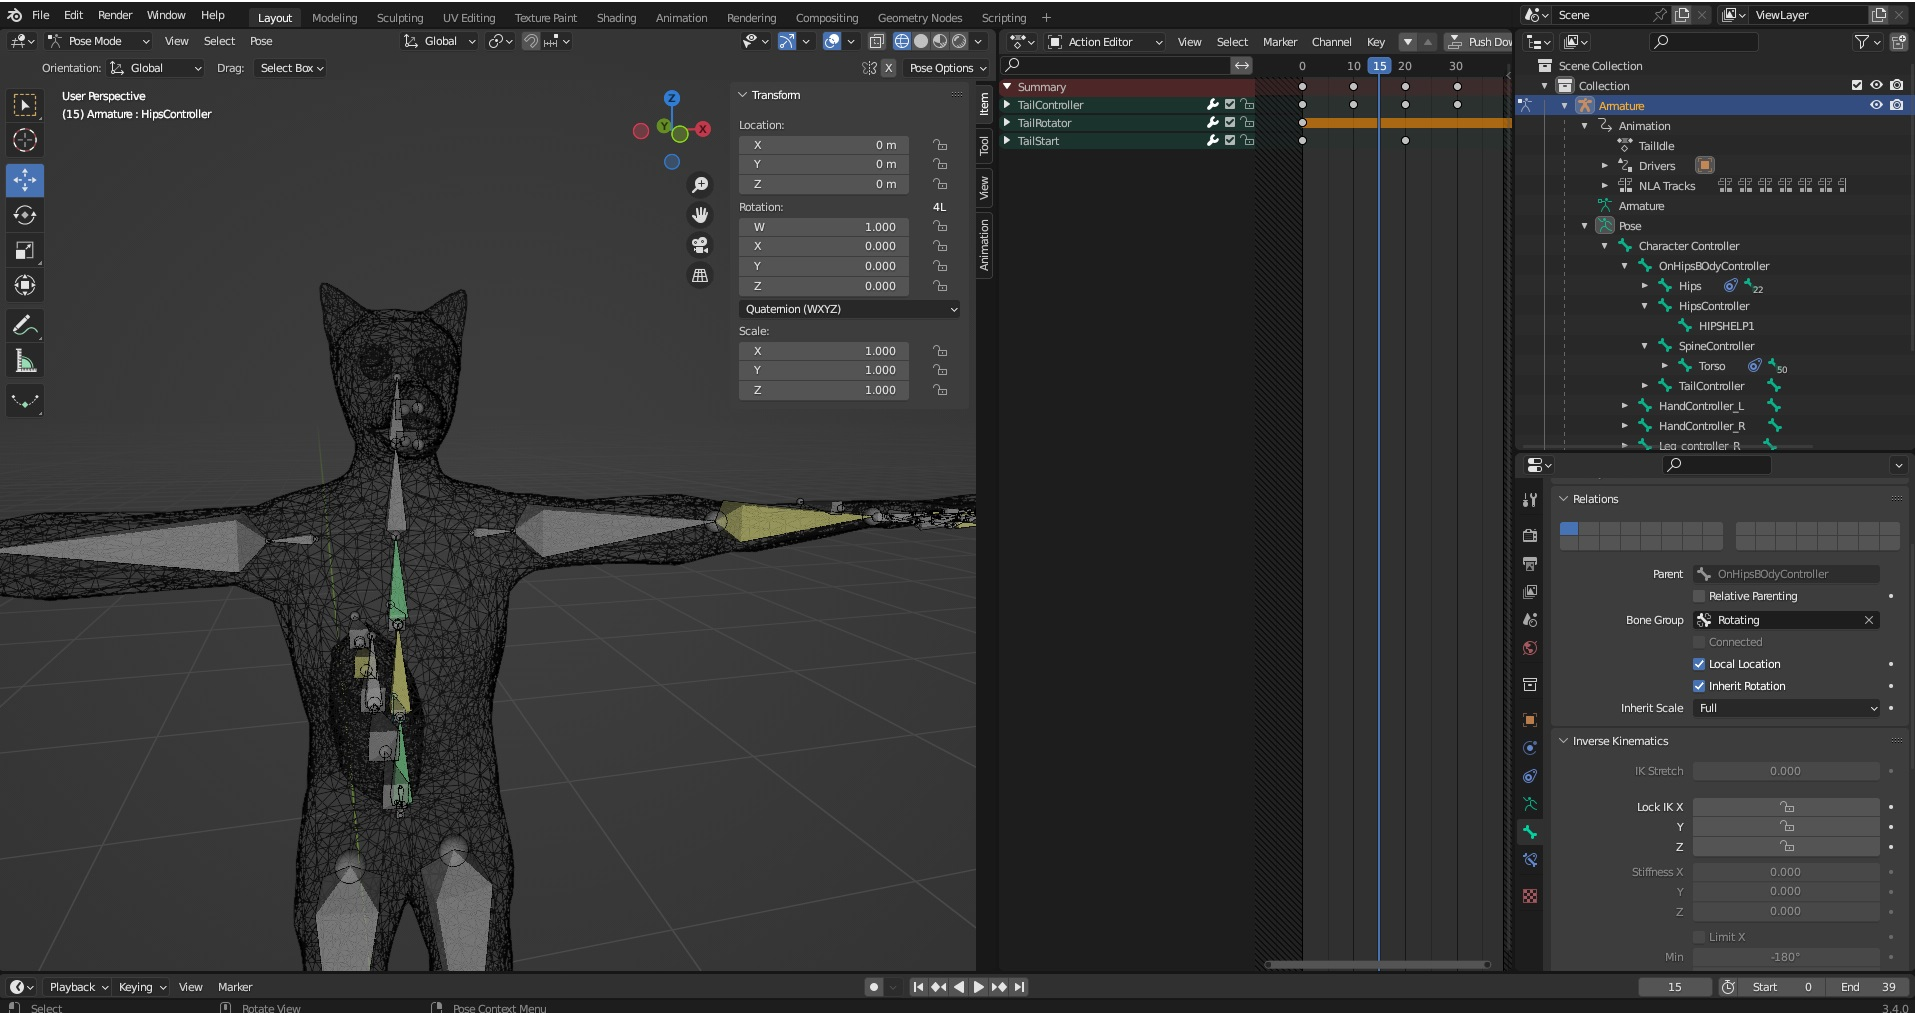
\includegraphics[width=12cm]{BlenderPict/WindowForAnimation.jpg}
    \caption{Zestaw pól roboczych używanych do animacji}
    \label{Blender:DefaulAnimationWin}
\end{figure}


Domyślnie 24 klatki oznaczają jedną sekundę animacji. Można to zmienić w polu
roboczym `Properties', w zakładce `Outpu Properties' zakładka `Format' pole
Frame Rate (pokazano na rysunku \ref{Blender:DefauitFrameRate}). Warto
zaznaczyć, że im większy `Frame Rate' tym większy będzie wyeksportowany plik,
ale animacje będą bardziej szczegółowe. 

\begin{figure}[ht!]
    \centering
    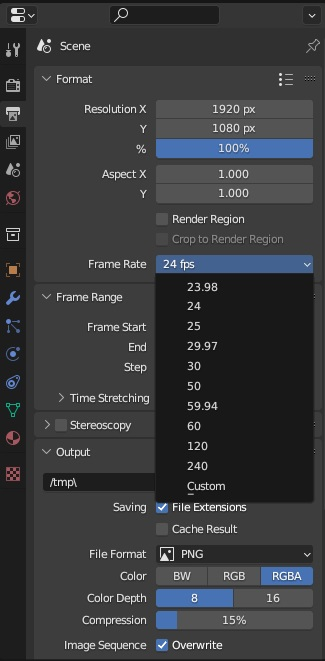
\includegraphics[width=6cm]{BlenderPict/Animation_FrameRate.jpg}
    \caption{Zmiana Frame Rate}
    \label{Blender:DefauitFrameRate}
\end{figure}

Przed rozpoczęciem animowania należy ustawić ile klatek ma trwać dana animacja –
domyślnie klatką początkową jest klatka 0, a końcową ostatnia zapisana klatka.
Na obranie \ref{Blender:Arrow} można zobaczyć strzałkę, które otwiera menu,
które pozwala na zmianę początku i końca animacji pokazanego na rysunku
\ref{Blender:ChangeStartFrame}. Poza tym można określić czy dana animacja jest
zapętlona -- pole "Cyclic Animation".

\begin{figure}[ht!]
    \centering
    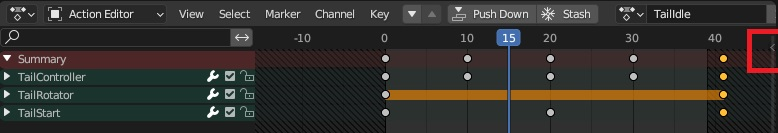
\includegraphics[width=6cm]{BlenderPict/ActionEditor_arrow.jpg}
    \caption{Strzałka prowadząca do menu pozwalającego na zmianę klatek początku i końca animacji}
    \label{Blender:Arrow}
\end{figure}


\begin{figure}[ht!]
    \centering
    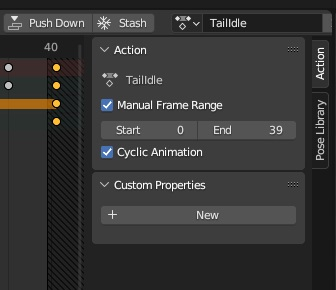
\includegraphics[width=6cm]{BlenderPict/ActionEditor_Frame_Range.jpg}
    \caption{Menu zmiany początku i końca animacji}
    \label{Blender:ChangeStartFrame}
\end{figure}

Zmiana klatki odbywa się poprzez kliknięcie na liczbę reprezentującą klatkę na
linii czasu (rysuneki \ref{Blender:TimeLine_a} i \ref{Blender:TimeLine_b} pola 1)
\begin{figure}[ht!]
    \centering
    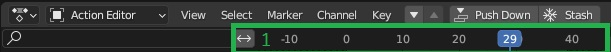
\includegraphics[width=12cm]{BlenderPict/TimeLine1.jpg}
    \caption{Linia czasu w polu roboczym Dope Sheet w trybie ActionEditor}
    \label{Blender:TimeLine_a}
\end{figure}

\begin{figure}[ht!]
    \centering
    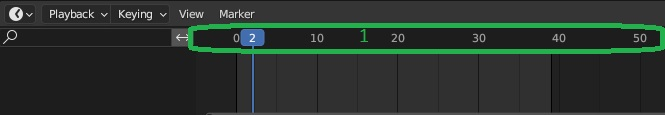
\includegraphics[width=12cm]{BlenderPict/TimeLine2.jpg}
    \caption{Linia czasu w polu roboczym TimeLine}
    \label{Blender:TimeLine_b}
\end{figure}


Kluczowanie klatek odbywa się  poprzez zaznaczenie kości -- jednej lub kilku -
wciśnięcie klawiska `I'. Wtedy pojawi się menu (rysunek
\ref{Blender:Insert_KeyFrame}), w którym można wybrać jakie wartości będą
zapisywane w klatce animacji. Warto wspomnieć o różnicach między poszczególnymi
opcjami kluczowania klatki. `Visual Location' zapisze lokację kości jaką widać
na podglądzie. Opcja ta jest używana głównie w przypadku używania modyfikatorów.
Zwykłe `Location' odnosi się do zmiany pozycji przez użytkownika. `Custom
Properties' mówi o innych właściwościach stworzonych przez użytkownika. `BBone
Shape' jest używany w przypadku specjalnych kości nazywanych `Bendy Bones'.
`Whole Character' kluczuje wszystkie właściwości wszystkich kości, jest to
rzadko używane.

\begin{figure}[ht!]
    \centering
    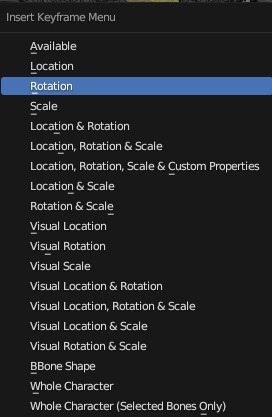
\includegraphics[width=8cm]{BlenderPict/Possible_Insert_KeyFrame.jpg}
    \caption{Menu wyboru zapisanych informacji do klatki animacji}
    \label{Blender:Insert_KeyFrame}
\end{figure}



\clearpage
\section{Przygotowanie modeli, animacji i tekstur}
Do projektu zostały przygotowane 2 modele z animacjami i teksturami –
ciernie i postać główna.

\subsection{Ciernie}
Model cierni został wykonany w stylu Low Polly -- bardzo mała ilość detali, model
może być kanciasty. Model został podzielony na 2 części -- grubsza i chudsza
część. Każda z tych części jest sterowana osobną kością. Zostały stworzone 3
animacje cierni -- `FastFloating', `SlowFloating' i `Touched'. `FastFloating'  i
`SlowFloating' są animacjami cyklicznymi i mają symulować wpływ wiatru na
ciernie. Animacja `Touched' jest zachowaniem się cierni na wypadek dotknięcia
ich przez postać główną. 
\begin{figure}[h!]
    \centering
    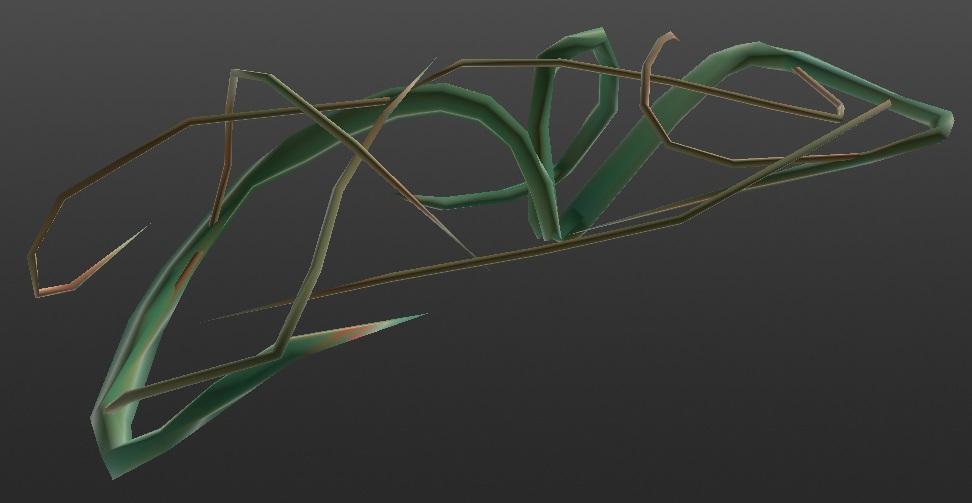
\includegraphics[width=12cm]{RealizacjaProjektu/Thorns/bramble_TEXT.jpg}
    \caption{Model cierni z nałożoną teksturą}
    \label{Bramble:Model}
\end{figure}
\subsubsection{Szkielet}
Szkielet jest bardzo prosty i składa się z 4 kości. Podstawową
kością, która służy do przemieszczania i rotowania całym modelem jest
`BasicBone'. Kości `SmallBrambles' i `BigBrambles' służą do poruszania
odpowiednio cieńszą i grubszą częścią. Kość `SteringBone' służy do poruszania
kośćmi `SmallBrambles' i `BigBrambles'

\begin{figure}[ht!]
    \centering
    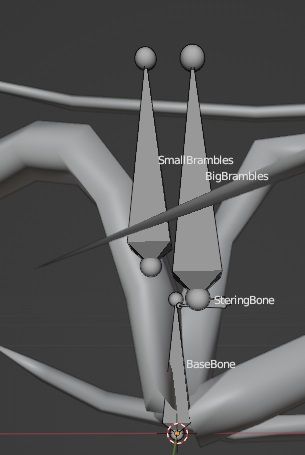
\includegraphics[width=7cm]{RealizacjaProjektu/Thorns/BrambleArmature.jpg}
    \caption{Położenie kości szkieletu cierni}
    \label{Bramble:Aramature}
\end{figure}
\begin{figure}[ht!]
    \centering
    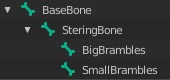
\includegraphics[width=7cm]{RealizacjaProjektu/Thorns/Bramble_ArmatrueHierarchy.jpg}
    \caption{Hierarchia kości dla skieletu cierni}
    \label{Bramble:ArmatrueHierarchy}
\end{figure}
\clearpage
\subsubsection{Weight Paint}

Kość `BaseBone' wpływa tylko na grubszą część modelu (rysunek
\ref{Bramble:WeightsRoot}). W ten sposób `Korzeń' modelu jest nieruchomy.
\begin{figure}[ht!]
    \centering
    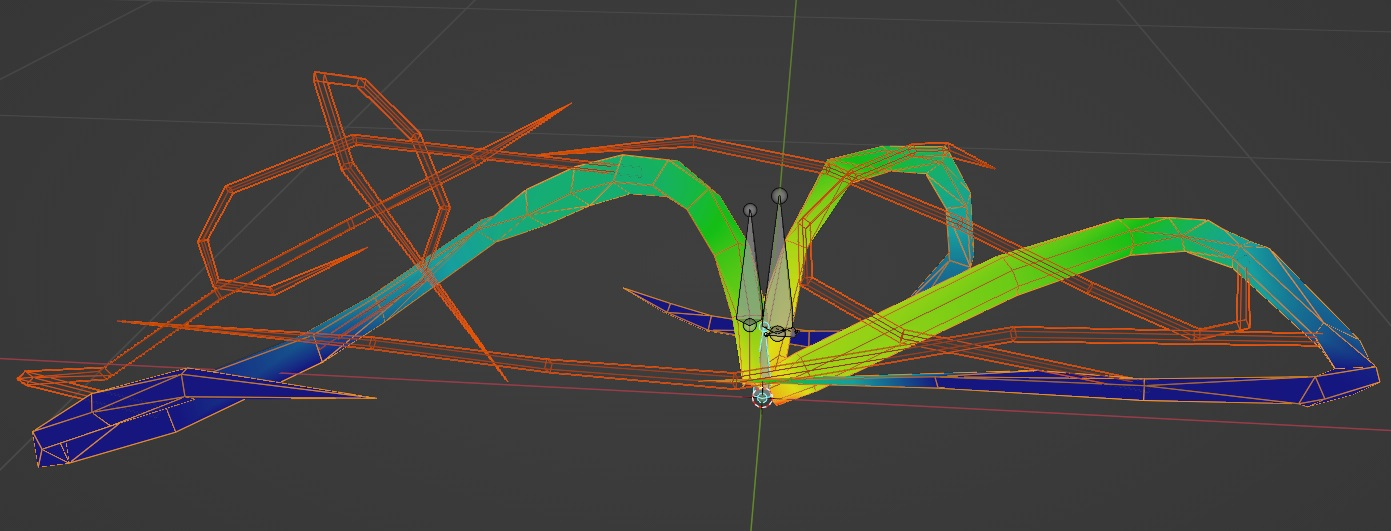
\includegraphics[width=12cm]{RealizacjaProjektu/Thorns/bramble_weight_root.jpg}
    \caption{Wpływ kości `BaseBone}
    \label{Bramble:WeightsRoot}
\end{figure}

Kość `BigBrambles' wpływa na 2 części modelu. Na rysunku
\ref{Bramble:WeightsBigBigBrambles} przestawiono mapę wag tej kości na modelu
grubszych cierni. Rysunek \ref{Bramble:WeightsSmallBigBrambles} przedstawia
wpływ tej kości na cieńszą część modelu. Takie rozwiązanie pozwoliło na
połączenie ze sobą tych dwóch części. Częstym problemem w animacjach jest
rozłączanie się modeli podzielonych na części.

\begin{figure}[ht!]
    \centering
    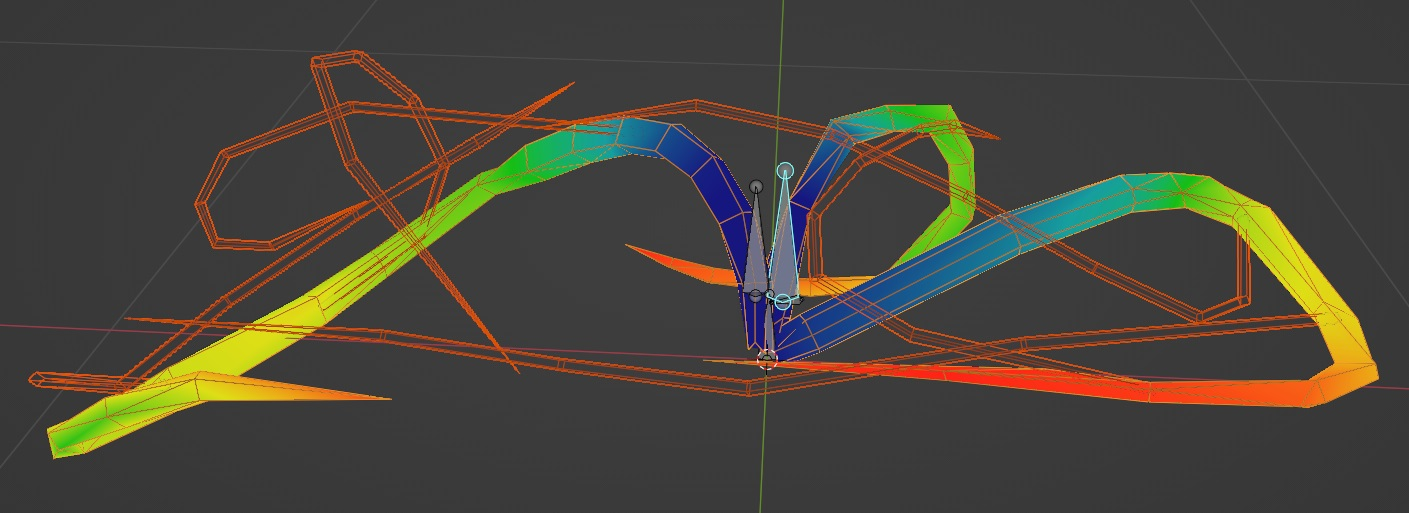
\includegraphics[width=12cm]{RealizacjaProjektu/Thorns/bramble_weight_Big_BigBrambles.jpg}
    \caption{Wpływ kości `BigBrambles na grubszą część modelu}
    \label{Bramble:WeightsBigBigBrambles}
\end{figure}
\begin{figure}[ht!]
    \centering
    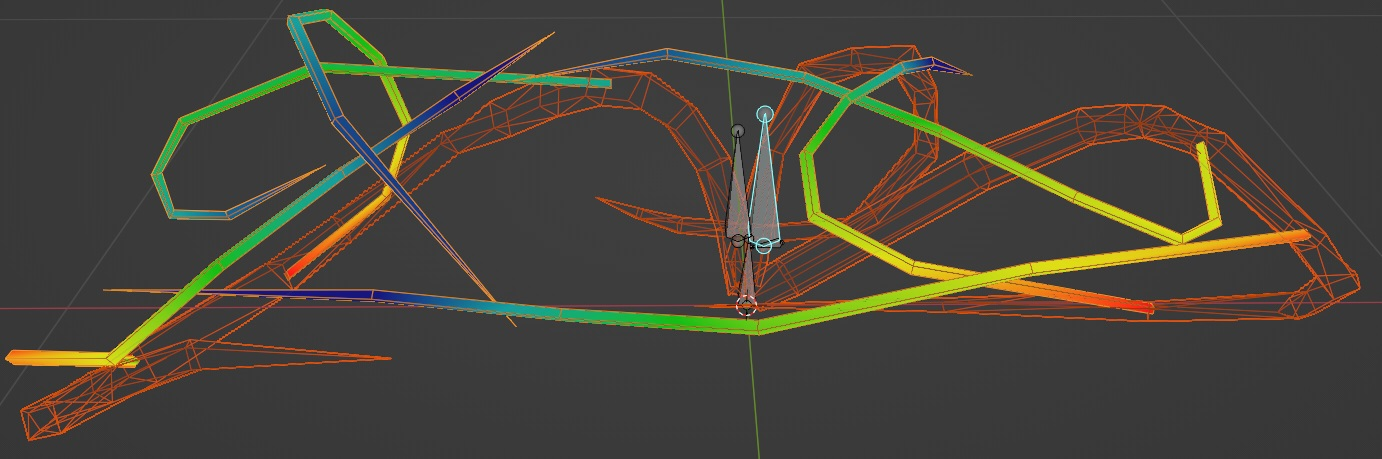
\includegraphics[width=12cm]{RealizacjaProjektu/Thorns/bramble_weight_Small_BigBrambles.jpg}
    \caption{Wpływ kości `BigBrambles na cieńszą część modelu}
    \label{Bramble:WeightsSmallBigBrambles}
\end{figure}

Kość `SmallBrambles` odpowiada za deformacje cieńszych gałęzi modelu. Pokazano
to na rysunku \ref{Bramble:WeightsSmallBrambles}.

\begin{figure}[ht!]
    \centering
    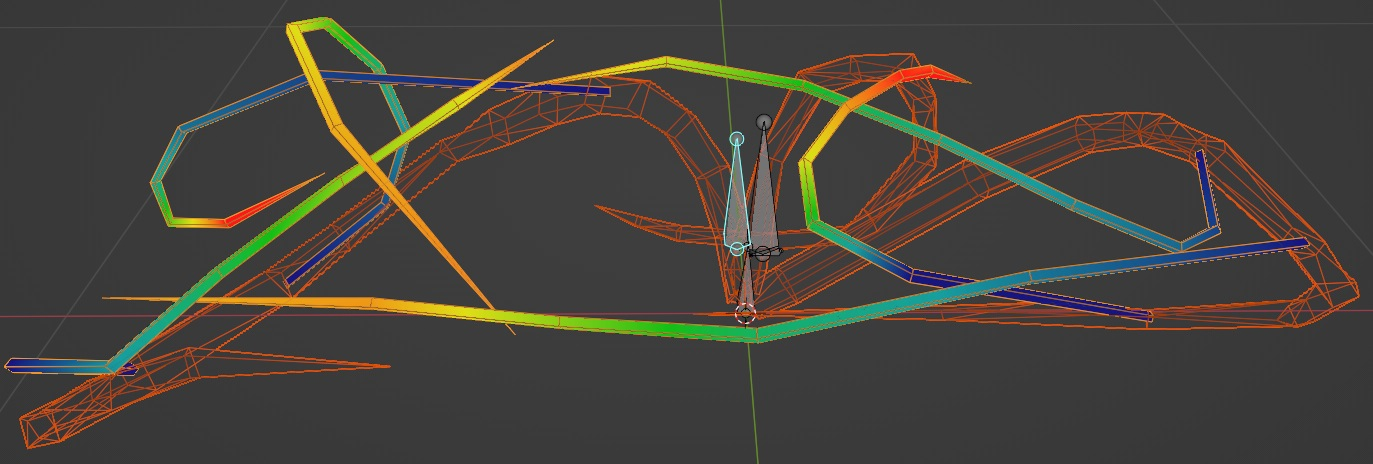
\includegraphics[width=12cm]{RealizacjaProjektu/Thorns/bramble_weight_SmallBrambles.jpg}
    \caption{Wpływ kości `SmallBrambles' model}
    \label{Bramble:WeightsSmallBrambles}
\end{figure}

\clearpage
\subsection{Postać główna}

Pozą spoczynkową -- w pozie spoczynkowej kości nie są transformowane -- jest tzw.
`T pose' -- postawa postaci przypomina literę T. Model postaci jest
skierowany twarzą wzdłuż osi Y. Powodem tego jest fakt, że edycja kości w programie
może działać lustrzanie, ale tylko w wypadku, gdy są one odbite lustrzanie wg.
osi Y. Jako wzór do zachowania pewnych proporcji -- np. stosunek rąk do tułowia –
został użyty obraz człowieka witruwiańskiego (rysunek \ref{VitruvianMan}).
Szkielet został lekko zniekształcony -- zostały wydłużone kończyny -- tak, aby
kształtem wyglądał jak wilkołak. Proces używania obrazu jako referencji został
pokazany w filmie \cite{blender_reference}. Krokiem pierwszym stworzenia postaci
głównej było zrobienie szkieletu, a następnie zrobienie modelu. W czasie
tworzenia animacji szkielet zmienił się kilka razy. Powody zmian zostały zawarte
w dziale o szkielecie postaci głównej.
\begin{figure}[h]

    \centering
	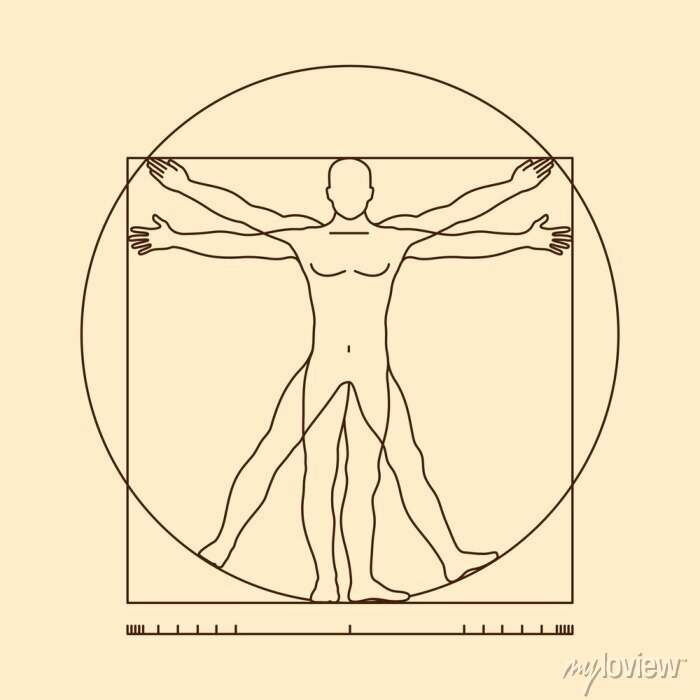
\includegraphics[width=6cm]{RealizacjaProjektu/MC/VitruvianMan.jpg}
	\caption{Szkic człowieka witruwiańskiego}
    \label{VitruvianMan}
\end{figure}

\subsubsection{Szkielet animacji}

Kości z końcówką L mają swój lustrzany odpowiednik R -- gdy zostanie stworzona
połowa szkieletu, to można ją symetrycznie odbić wzłuż osi Y, a nazewnictwo jest
wymagane, bo w przeciwnym razie kości nie są lustrzanie odbijane. Kości zostały
podzielone na 2 grupy: kości deformujące i kości kontrolujące. Kości
kontrolujące kontrolują za pomocą modyfikatorów kości kilka kości na raz (lub
jedną w bardzo specyficzny sposób). Modyfikator IK (Inverse Kinematic) został
użyty do kontroli palców, rąk i nóg. Inverse Kinematic jest skomplikowanym
modyfikatorem i używanie go do animacji wielu kości, które mogą być rotowane
wokół wielu osi może doprowadzić do niechcianych ruchów. W przypadku kręgosłupa
zamiast 24 kręgów zastosowano 5 kości -- kość deformująca głowę (Head), kark
(Neck),  klatkę piersiową (Torso), biodra(Hips) i jedna kość między biodrami a
klatką piersiową (Spine\_2) -- co zostanie bardziej szczegółowo omówione w
dalszej części pracy. Kość `CharacterConteroller' została użyta do transformacji
wszystkich kości, a kość `OnHipsBOdyController' do transformacji bez kości
`HandCOntroller' i `LegController'. Jest to spowodowane potrzebą odseparowania
kończyn -- nóg i rąk -- od reszty ciała. Hierarchia kości szkieletu została
przedstawiona na rysunkach
\ref{Aramature:BoneHierarchy1} i \ref{Aramature:BoneHierarchy2}.
\begin{figure}[hbt!]

    \centering
	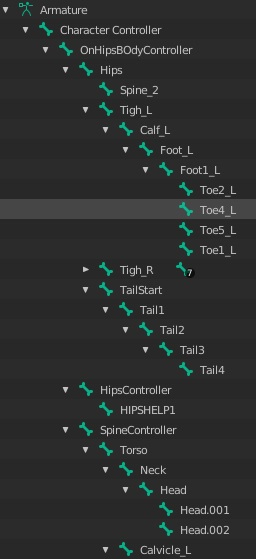
\includegraphics[width=6cm]{RealizacjaProjektu/MC/BoneHierarchy1.jpg}
	\caption{Hierarchia kości część 1}
    \label{Aramature:BoneHierarchy1}
\end{figure}
\begin{figure}[hbt!]

    \centering
	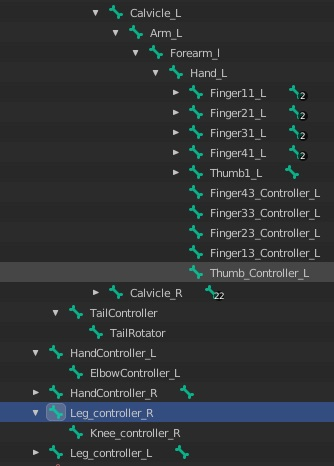
\includegraphics[width=6cm]{RealizacjaProjektu/MC/BoneHierarchy2.jpg}
	\caption{Hierarchia kości część 2}
    \label{Aramature:BoneHierarchy2}
\end{figure}
\hspace{0.10cm}
\linebreak
\linebreak
\linebreak
\linebreak
\linebreak
Żółte kości na rysunkach \ref{Aramature:HandBones}, \ref{Aramature:UpperBody} i
\ref{Aramature:LowerBody} posiadaja modyfikator IK, a na zielono posiadające
modyfikator `CopyTransform' lub `CopyLocation'. Kości, które są modyfikowane przez
modyfikator IK z kością `Pole Target' nie mogą być w jednej osi. Większość kości
otrzymała maksymalny kąt zgięcia w danej osi pod wpływem modyfikatora IK, co
pozwoliło na np. bardziej realistyczne zginanie się kości. Opcja ta jest
dostępna w polu roboczym `Properties' -> `Bone Properties' -> zakładka `Inverse
Kinematics' -> opcje `Limit X',  `Limit Y' i `Limit Z'. Było to bardzo użyteczne
podczas np. zginania ręki w łokciu -- ręka w łokciu może się zginać tylko w
jednym kierunku, a rotacja ramienia odbywa się w chrząstce między kością
ramieniową, a obojczykiem. Na zasadzie obserwacji i metody prób i błędów udało
się ustalić maksymalne kąty zgięcia w danym miejscu. Nie działa to perfekcyjnie,
ale bardzo ułatwia pracę podczas tworzenia animacji. Blender posiada błąd, który
powoduje, że modyfikator nie działa w takim wypadku poprawnie. Do obracania
całej dłoni służy kość `Hand', która ją też deformuje. Każdy z palców dłoni –
poza kciukiem, który składa się z 2 kości -- składa się z 3 kości deformujących
sterowanych jedną kością -- np. `Finger33\_Controller\_R' -- za pomocą
modyfikatora IK. Kontrolery palców za rodzica mają kość nadgarstka.
Sterowaniem całą ręką -- 2 kości, na kość obojczyka `calvicle' nie ma wpływu -
zajmuje się kość `HandController' za pomocą modyfikatora IK przypiętego do kości
`Forearm'. Rodzicem kości `HandController' jest kość główna `Character
Controller'. Jako kość rotacyjna ustawiona jest kość `ElbowController', której
rodzicem jest kość `HandController'. 

\begin{figure}[h]
    \centering
	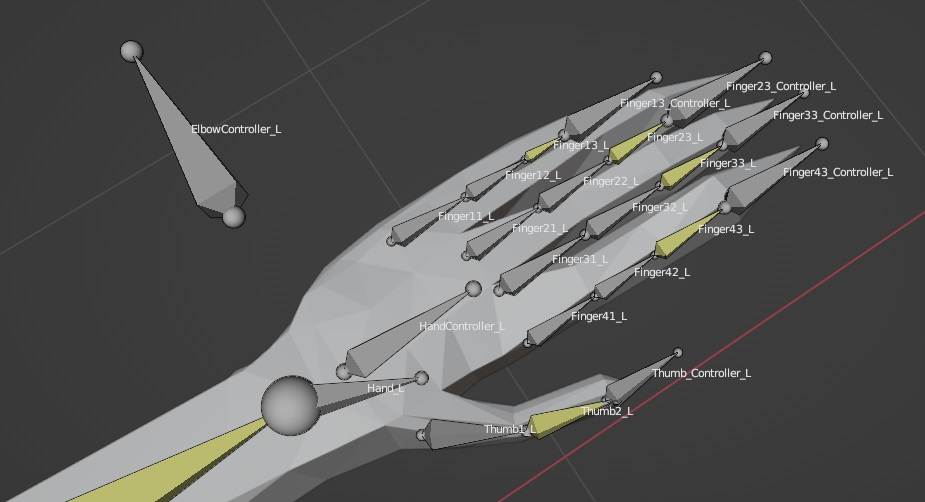
\includegraphics[width=10cm]{RealizacjaProjektu/MC/Bones_Hand.jpg}
	\caption{Kości Ręki}
    \label{Aramature:HandBones}
\end{figure}

Kości kręgosłupa są
sterowane inaczej niż kości nóg czy rąk. Kręgosłup jest częścią ciała, która
jest najbardziej giętka i dynamiczna. W porównaniu do kończyn dolnych i górnych
wymaga większej kontroli. Zastosowanie sterowania za pomocą pojedynczego
modyfikatora IK powodowało problemy -- lekkie poruszanie powodowało bardzo duże
zmiany w transformacjach kości. Dlatego na podstawie filmu
\cite{blender_Better_Spine} został zaimplementowany układ sterowania tułowiem.
Nowy układ pozwala na swobodne sterowanie odpowiednimi częściami tułowia.
Do sterowania deformacją w okolicach klatki piersiowej i bioder służą kości
`SpineController` i `HipsController` (rysunek \ref{Aramature:UpperBody}). 

\begin{figure}[h]
    \centering
	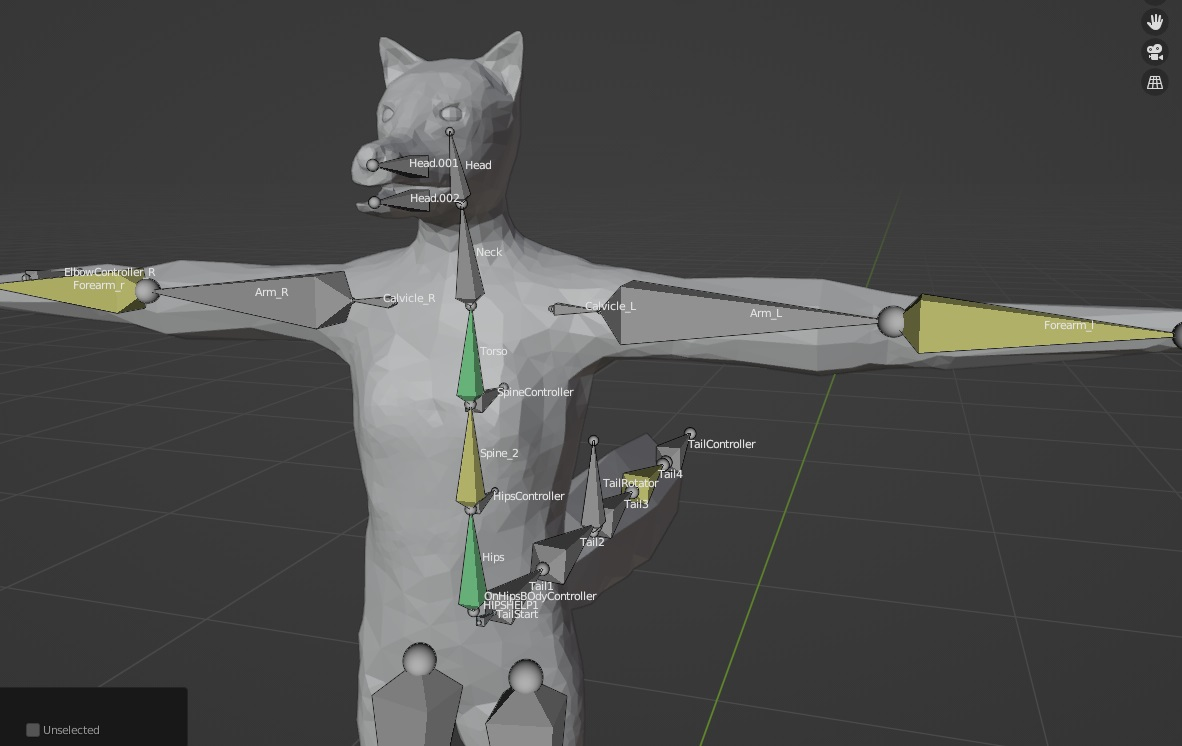
\includegraphics[width=10cm]{RealizacjaProjektu/MC/Bones_upperBody.jpg}
	\caption{Kości górnej części ciała}
    \label{Aramature:UpperBody}
\end{figure}

Sterowaniem nogą są używane 2 kości -- kość kontrolera `Leg\_controller' i kość
służąca do rotacji `Knee\_controller' -- które sterują dwoma kośćmi -- `Tigh' i
`Calf'. Stopa składa się z dwóch kości i każda animowana jest osobno oraz kości
palców, które nie są używane do animacji. 

\begin{figure}[!h]
    \centering
	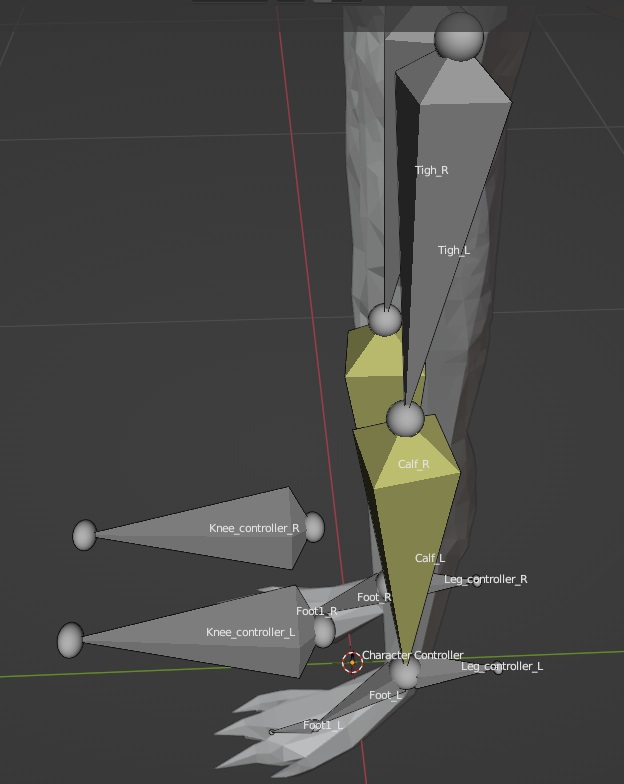
\includegraphics[width=9cm]{RealizacjaProjektu/MC/Bones_LowerBody.jpg}
	\caption{Kości dolnej części ciała}
    \label{Aramature:LowerBody}
\end{figure}

Ogon składa się z 7 kości -- 5 kości deformujących, kości sterującej
`TailContoller' i kości rotującej `TailRotator'. `TailController' steruje 4 z 5
kości deformujących -- kosci `Tail1-4', gdzie `Tail4' jest kością końcową. Kość
`TailStart' posłużyła do poprawnego ułożenia ogona względem ciała -- np. podczas
animacji biegu tułów i ogon powinny znajdować się w jednej płaszczyźnie.

\begin{figure}[!h]
    \centering
	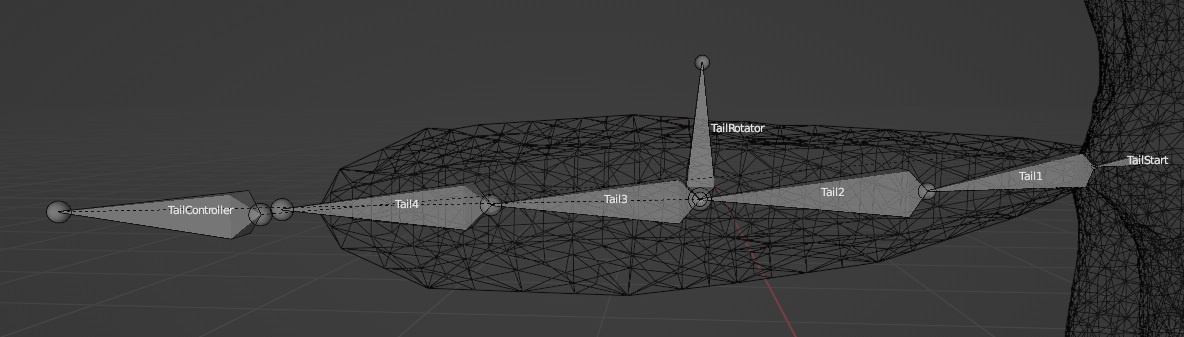
\includegraphics[width=10cm]{RealizacjaProjektu/MC/Armature_tail.jpg}
	\caption{Kości ogona postaci}
    \label{Aramature:Tail}
\end{figure}

\clearpage 
\subsubsection{Model i Tekstury}
Model postaci (wraz z teksturami na rysuneku\ref{Texture:FrontMC} i
rysunku \ref{Texture:QuixelMixer}) został przygotowany w stylu medium poly -
określenie na modele graficzne posiadające od 1000 do 15000 ścian, cechuje się
ilością detali. Model miejscami jest kanciasty, a częściami ciała, na których to
najbardziej widać są: dłonie (rysunek \ref{MC:Hand}), stopy(rysunek
\ref{MC:Foot}) i ogon \ref{MC:Tail}. W grze dłonie i stopy są mało widoczne,
przez co nie jest to widoczne. Ogon mimo posiadania wielu punktów nie został
dobrze `wyrzeźbiony'. Ogon postaci wymagał bardziej skomplikowanej siatki ze
względu na animacje.

Przed przystąpieniem do robienia tekstur należy zrobić `UV maping'. Tekstury są
dwu-wymiarowymi mapami nałożonymi na trójwymiarowy obiekt. Proces nakładania
tekstur można porównać do procesu oklejania papierem obiektu. W niektórych
przypadkach obiekt można okleić bez cięcia papieru. W większości przypadków
papier trzeba pociąć wiele razy.  Blender do tego celu posiada zestaw pól roboczych
– `UV Editing'. Na rysunkach \ref{MC:Hand}, \ref{MC:Foot} i \ref{MC:Tail} na czerwono oznaczono
cięcia, które będą zachodzić podczas generowania mapy UV. Proces ten bardzo
dobrze opisany -- wraz z rzeczami, na które należy uważać -- został w filmach
\cite{blender_UV_editing_advanced} i \cite{blender_UV_editing_simple}.

\begin{figure}[!h]
    \centering
	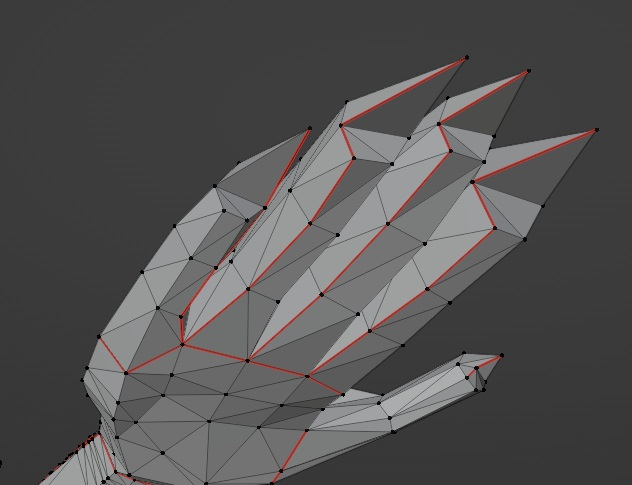
\includegraphics[width=10cm]{RealizacjaProjektu/MC/Model_hand.jpg}
	\caption{Ręka postaci głównej}
    \label{MC:Hand}
\end{figure}
\begin{figure}[!ht]
    \centering
	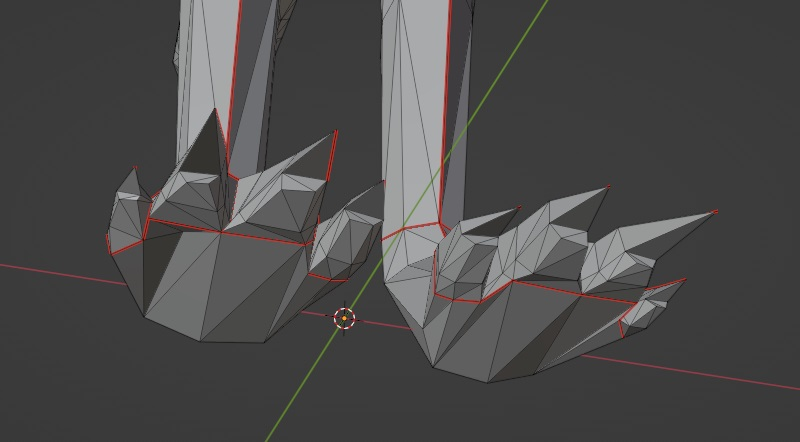
\includegraphics[width=10cm]{RealizacjaProjektu/MC/Model_feet.jpg}
	\caption{Stopa postaci głównej}
    \label{MC:Foot}
\end{figure}
\begin{figure}[!ht]
    \centering
	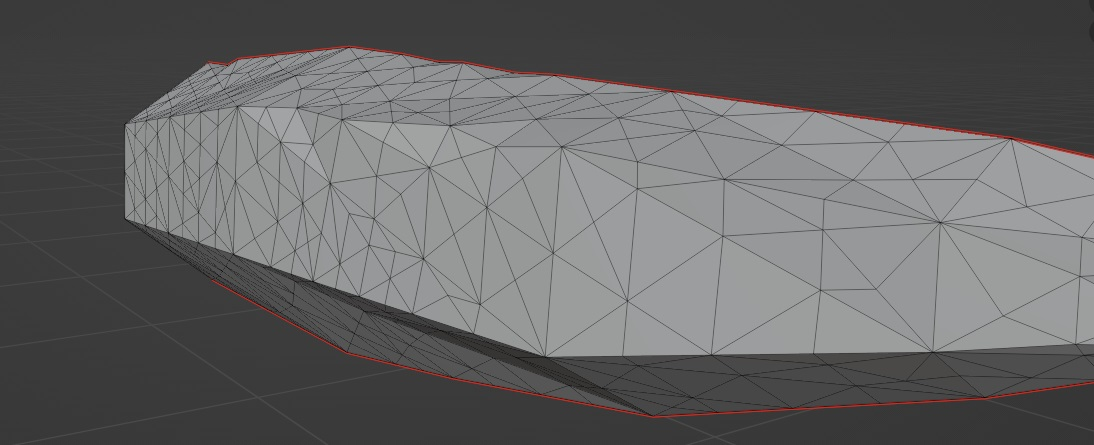
\includegraphics[width=12cm]{RealizacjaProjektu/MC/model_tail.jpg}
	\caption{Ogon postaci głównej}
    \label{MC:Tail}
\end{figure}
\clearpage
Tekstury zostały wykonane w programie Quixel Mixer (rysunek
\ref{Texture:FrontMC}). Tekstury zostały wykonane w programie Quixel Mixer.
Program działa podobnie do programu Gimp -- tworzenie grafik za pomocą warstw,
ale dla modeli 3D. Program przyjmuje model stworzony za pomocą innych programów
np. Blender lub Maya w formacie FBX.  Największym problemem programu jest jego
prędkość działania -- wymaga on mocnej karty graficznej.

\begin{figure}[!h]
    \centering
	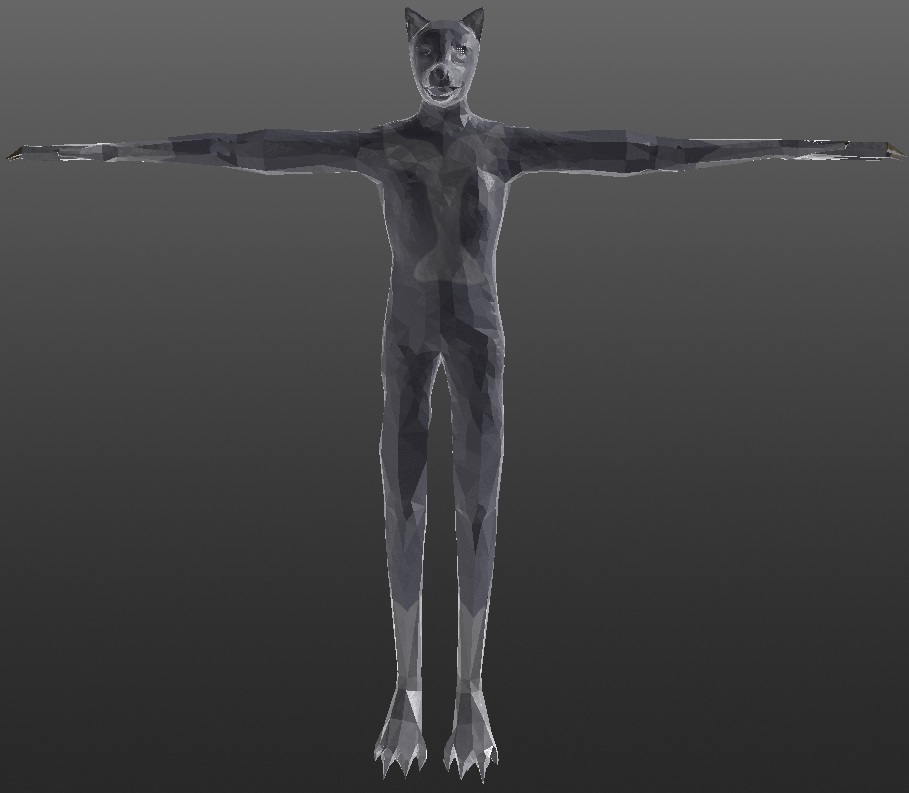
\includegraphics[width=12cm]{RealizacjaProjektu/MC/TexturedMC_Front.jpg}
	\caption{Oteksturowana postać -- widok od przodu}
    \label{Texture:FrontMC}
\end{figure}

Po lewej stronie rysunku \ref{Texture:QuixelMixer} znajdują się warstwy. Ikona folderu oznacza
grupę. Każda warstwa, która znajduje się w grupie, maluje tylko obszar dozwolony
przez maskę w grupie. Maska może być wygenerowana -- za pomocą szumów -- lub
malowana ręcznie. Każda warstwa może posiadać: poziom przezroczystości -- ten
zawsze musi być zdefiniowany -- kolor, metalowość, chropowatość i kilka innych.
Każdy z tych atrybutów może przyjmować wartość od 0 do 1. Materiałem może być
też sam szum, który może wpływać na materiały poniżej niego. Materiał lub grupa,
która jest najwyżej będzie najbardziej na wierzchu.

\begin{figure}[!ht]
    \centering
	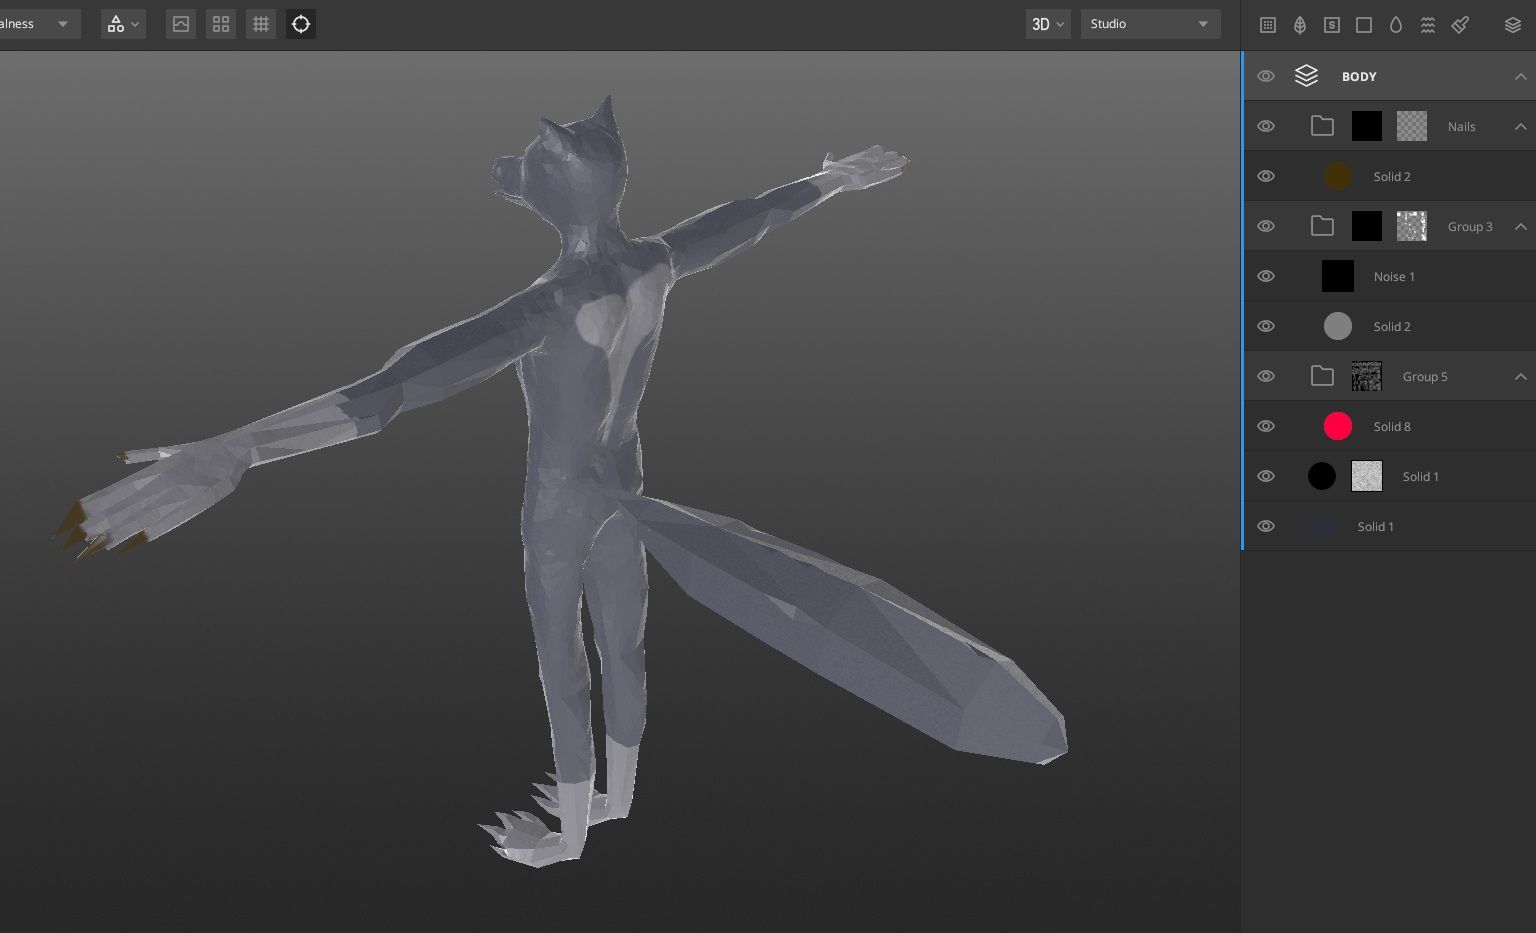
\includegraphics[width=10cm]{RealizacjaProjektu/MC/Texture_QuixelMixer.jpg}
	\caption{Postać główna w QuixelMixer}
    \label{Texture:QuixelMixer}
\end{figure}



\subsubsection{Animacje}

Animowanie są tematem złożonym, którego nie da się opisać w prosty sposób, a
samo tworzenie animacji jest zależne od wielu czynników. Pierwszym krokiem przed
rozpoczęciem animowania powinna być obserwacja ruchów zwierząt lub ludzi, którzy
wykonują podobne ruchy, jakie mają znaleźć się w animacji. W dzisiejszych
czasach, gdzie internet jest ogólnodostępny jest to proces jedynie czasochłonny.
Obserwowany ruch następnie należy rozbić na etapy, a w każdym etapie rozbić ruch
na części ciała -- np. nogi, ręce tułów, głowa. Przykładowo chód ludzi -- bez
brania pod uwagę momentu startu i momentu stopu -- ruch nóg można podzielić na 7
etapów -- w uproszczeniu -- gdzie jeden etap się powtarza:
\begin{itemize}
\item rozkrok dla uproszczenia lewa noga jest z tyłu, biodra znajdują się w najniższym możliwym punkcie (podczas chodu), lewa  ręka jest wysunięta do przodu, prawa ręka jest wysunięta do tyłu
\item podniesienie nogi lewej, przeniesienie punktu ciężkości ciała na prawą nogę, co powoduje lekkie przechylenie w prawo
\item noga lewa wyprzedza nogę prawą , biodra znajdują się w najwyższym możliwym puncie (podczas chodu), maksymalnie przychylenie ciała w prawo
\item postawienie nogi lewej, nogi ponownie znajdują się w rozkroku prawa ręka wysunięta do przodu, prawa ręka wysunięta w tył, biodra znajdują się w najniższym możliwym punkcie (podczas chodu)
\item podniesienie nogi prawej, przeniesienie punktu ciężkości ciała na lewą nogę, co powoduje lekkie przechylenie w lewo
\item noga prawa wyprzedza nogę lewą, biodra znajdują się w najwyższym możliwym puncie, maksymalnie przychylenie ciała w prawo
\item rozkrok dla uproszczenia lewa noga jest z tyłu, biodra znajdują się najniżej, lewa  ręka jest wysunięta do przodu, prawa ręka jest wysunięta do tyłu -- powrót do pozycji startowej
\end{itemize}
Dla bardziej zaawansowanych animacji taka rozpiska będzie bardziej obszerna –
będzie zawierać informacje o np. napięciach mięśni. Niestety dla animacji twarzy
taka rozpiska jest ciężka do zrobienia i zwykle twórcy te animacje robią metodą
`motion capture' lub `na czuja'. Każdy z tych etapów będzie kluczowaną klatką. W
trakcie animowania należy zwracać uwagę na synchronizację między częściami
ciała.  Trzeba zwrócić uwagę czy dana animacja ma być zapętlona czy nie. W
przypadku zapętlonych animacji ostatnią klatką animacji -- dlatego klatki stop i
start powinny być ustawiane ręcznie -- nie może być pozycja startowa, ponieważ
dojedzie do podwojenia klatki -- postać nienaturalnie zatrzyma się. 

Ostatnim etapem powinno być ustawienie czasu trwania poszczególnych etapów. Dla wyżej
podanego przykładu, czas podniesienia między postawieniem nogi prawej, a
podniesieniem nogi lewej powinien być bardzo krótki. Czas między podniesieniem,
a postawieniem nogi powinien być najdłuższą częścią animacji -- ok. 45\% czasu
animacji dla jednej nogi, czas liczony od początku do końca animacji. W
programach graficznych jest możliwa edycja przebiegu animacji określonych kości
między kluczowanymi klatkami -- pole robocze `Graph Editor' (rysunek
\ref{Animation:GraphEditor}). W edytorze grafów można bardziej precyzyjnie
ustawić wartości zmieniane w danej chwili. Jest to szczególnie przydatne w
trakcie obracania obiektów. Kwaterniony są systemem reprezentacji obrotu wokół
pewnej osi i ten system jest bardziej rekompensuje wady zastosowania rotacji
przez macierze rotacji. Normalizacja kwaternionów powoduje przejście zmiennej w
przestrzeni w -- odpowiedzialnej za kąt obrotu -- z -1 do 1. W obliczeniach
matematycznych nie robi to wielkiej różnicy, ale w przypadku animacji, gdy
obiekt kręci się wokół osi może doprowadzić do obrotu w inną stronę. Dlatego
przy pomocy edytora grafów można zmienić tę wartość tak, aby została przy
wartości -1. 
\begin{figure}[!h]
    \centering
	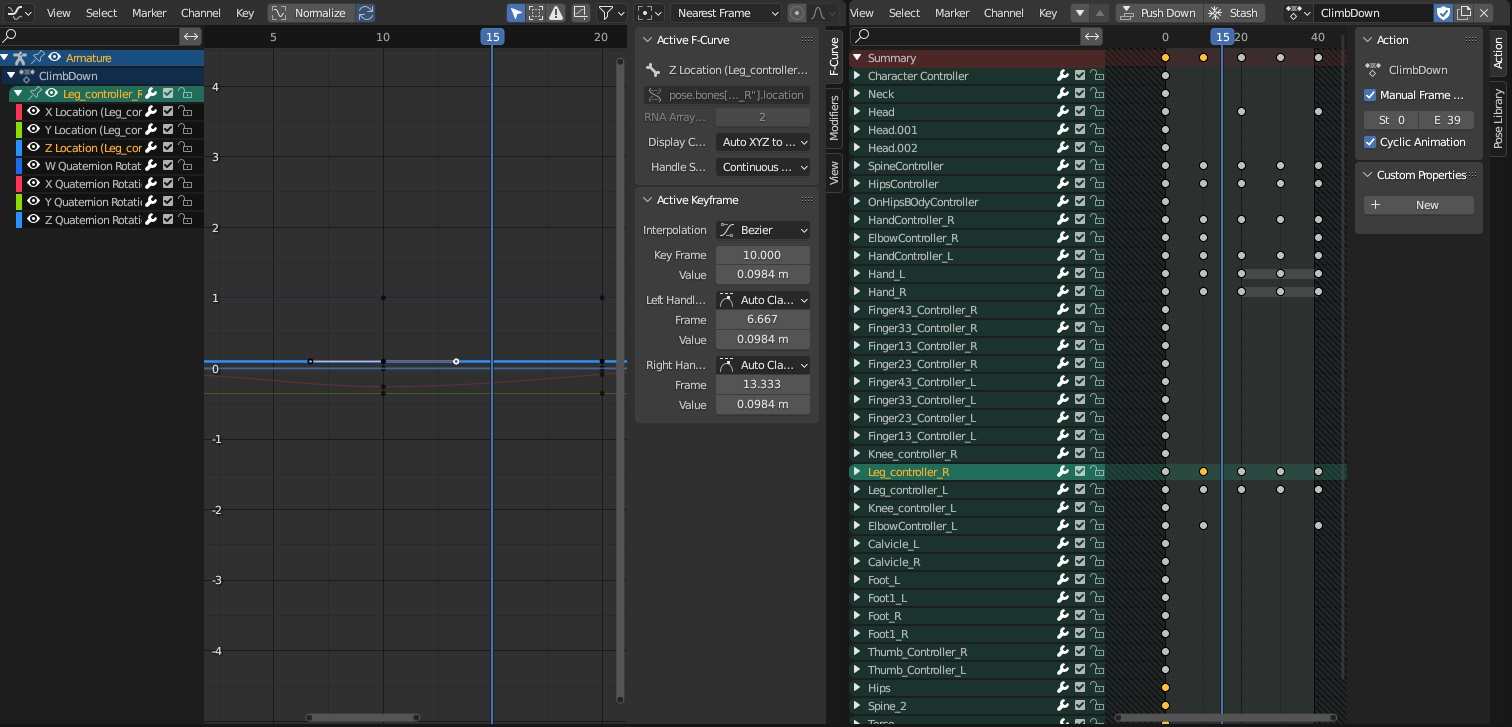
\includegraphics[width=10cm]{RealizacjaProjektu/MC/Animation_Graph_Editor.jpg}
	\caption{Edytor grafów w programie Blender}
    \label{Animation:GraphEditor}
\end{figure}
\linebreak
\linebreak
W animacji o nazwie `NextJump' postać robi przewrót w przód w powietrzu (rysunek
\ref{Animation:NextJumpProblem}). Problemem okazało się znormalizowanie
kwaternionu kości `OnHipsBOdyController' i postać zamiast przejść do pozycji
wyjściowej animacji zrobiła obrót w przeciwną stronę. Najlepszym rozwiązaniem
okazała się edycja przebiegu wartości `W' rotacji -- na dolnej części rysunku
\ref{Animation:NextJumpProblem} przedstawiono poprawioną wersję przebiegu
zmiennej. 

\begin{figure}[!ht]
    \centering
	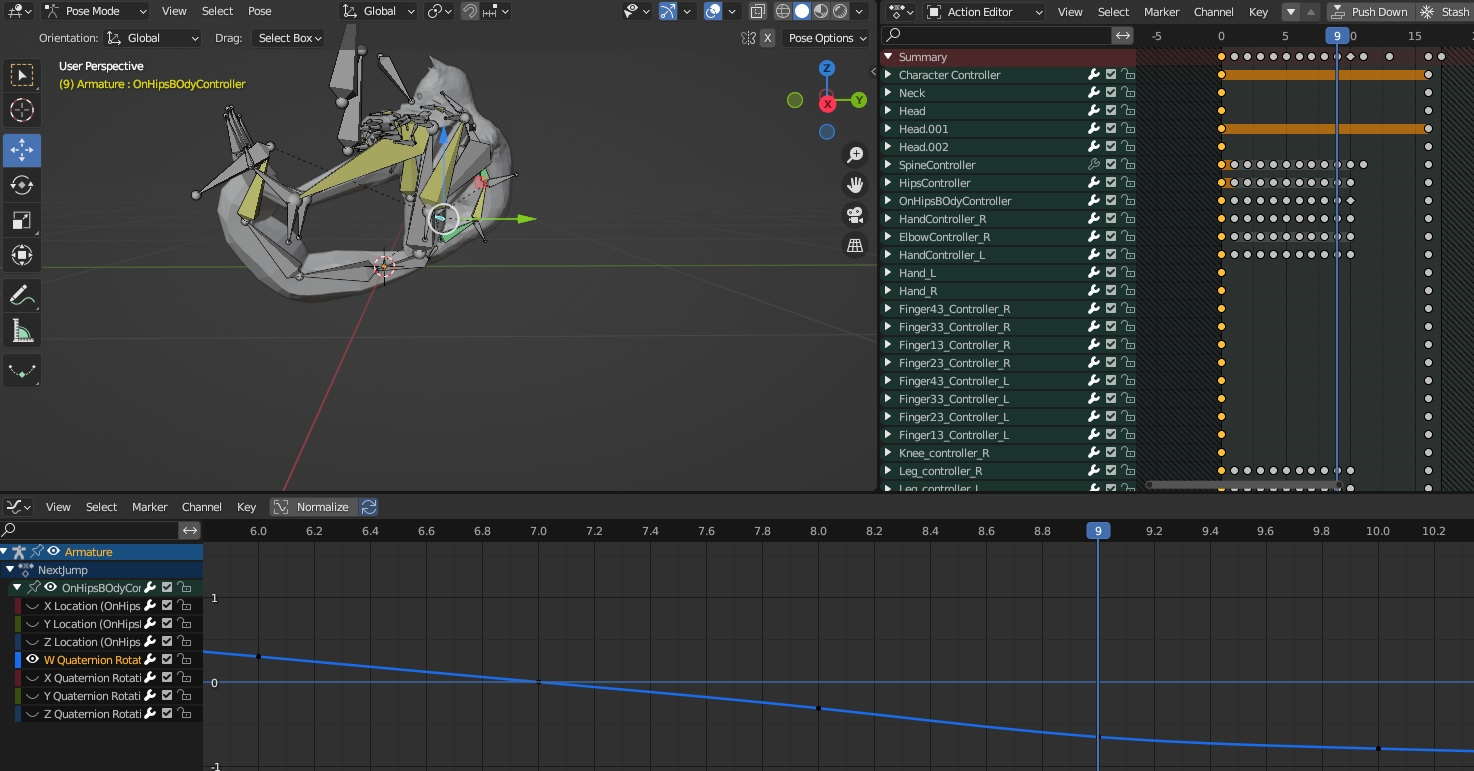
\includegraphics[width=10cm]{RealizacjaProjektu/MC/Animation_NextJump_problem.jpg}
	\caption{Animacja 'NextJump' z edytorem grafów}
    \label{Animation:NextJumpProblem}
\end{figure}

Poza tym postać główna posiada 18 innych animacji:
\begin{itemize}
\item Animacja `Idle' -- postać czeka (pokazano na rysunku \ref{Animation:Idle})
\item Animacja chodzenia (rysunek \ref{Animation:MoveLoop}) i biegu (rysunek \ref{Animation:Sprint})
\item Animacje ogona -- animacja spoczynku ogona i 4 animacje związane z ruchem postaci
\item Animacja skoku
\item Animacje wspinania (rysunek\ref{Animation:ClimbWait}) i podciągnięcia na krawędzi (rysunek \ref{Animation:ClimbOnEdge})
\item Animacja spadania
\item Animacja śmierci postaci (rysunek \ref{Animation:Death})
\end{itemize}

\begin{figure}[!ht]
    \centering
	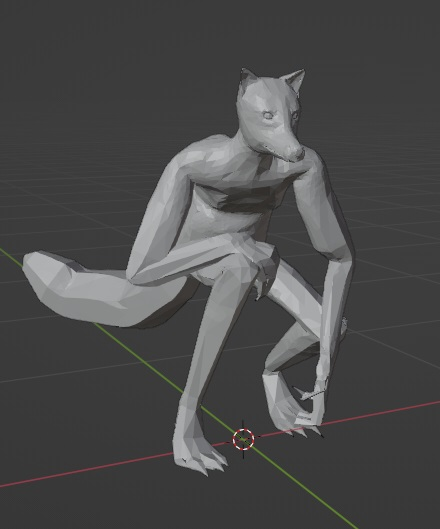
\includegraphics[width=9cm]{RealizacjaProjektu/MC/Animation_Idle_pose.jpg}
	\caption{Animacja 'Idle' -- postać oczekuje stojąc na ziemi}
    \label{Animation:Idle}
\end{figure}

\begin{figure}[!ht]
    \centering
	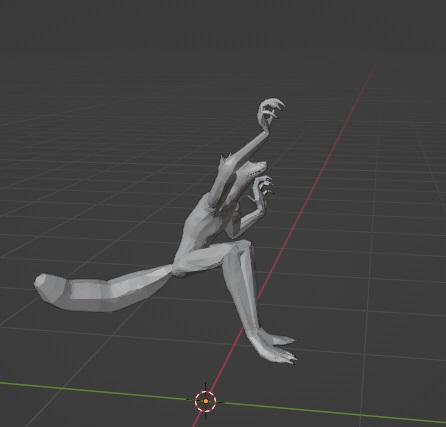
\includegraphics[width=10cm]{RealizacjaProjektu/MC/Animation_Climb_Wait.jpg}
	\caption{Animacja 'ClimbWait' -- oczekiwanie podczas wspinania}
    \label{Animation:ClimbWait}
\end{figure}
\begin{figure}[!ht]
    \centering
	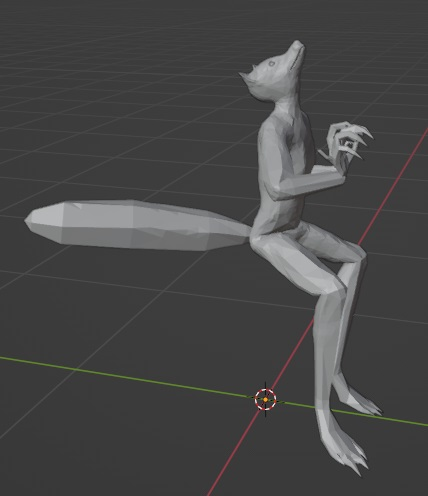
\includegraphics[width=10cm]{RealizacjaProjektu/MC/Animation_ClimbOnEdge.jpg}
	\caption{Animacja 'ClimbOnEdge' -- aniamcja podciągnięcia na krawędzi }
    \label{Animation:ClimbOnEdge}
\end{figure}
\begin{figure}[!ht]
    \centering
	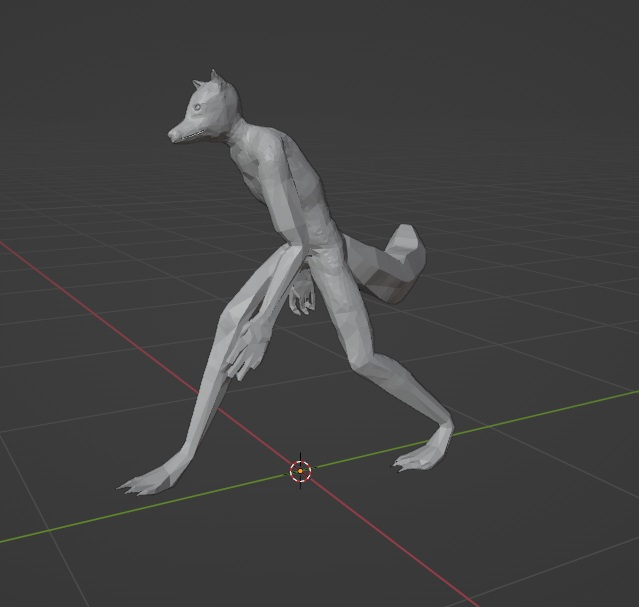
\includegraphics[width=10cm]{RealizacjaProjektu/MC/Animation_Move_Loop.jpg}
	\caption{Animacja 'MoveLoop' -- animacja chodu postaci}
    \label{Animation:MoveLoop}
\end{figure}
\begin{figure}[!ht]
    \centering
	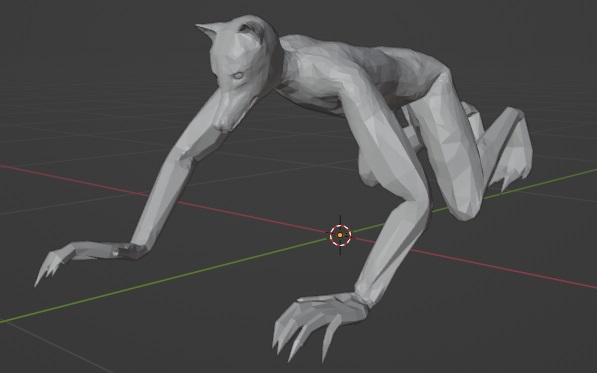
\includegraphics[width=10cm]{RealizacjaProjektu/MC/Animation_Sprint.jpg}
	\caption{Animacja 'Spring' -- animacja biegu postaci}
    \label{Animation:Sprint}
\end{figure}
\begin{figure}[!ht]
    \centering
	\includegraphics[width=10cm]{RealizacjaProjektu/MC/Animation_Death.jpg}
	\caption{Animacja 'Death' -- animacja śmierci postaci}
    \label{Animation:Death}
\end{figure}
\clearpage
\subsection{Eksportowanie modeli z animacjami}
Pliki .blend mogą być używane bezpośrednio przez silnik unity, ale nie działa to
poprawnie z animacjami. W tym celu należy ręcznie wyeksportować model z
animacjami do pliku FBX. W tym celu należy przejść do zakładki
`File'->'Export'->'FBX' (rysunek \ref{ExportFBX}).
\begin{figure}[!ht]
    \centering
	\includegraphics[width=10cm]{RealizacjaProjektu/Export/ExportFBX.jpg}
	\caption{Eksportowanie pliku FBX}
    \label{ExportFBX}
\end{figure}

Na rysunku \ref{ExportFBXOptions} zostały pokazane zalecane opcje eksportu
modelu z animacjami. W zakładce `Include' należy zaznaczyć `VisibleOBjects'
przez co zostaną wyeksportowane obiekty, które są widoczne -- obiekty można ukryć
za pomocą klawisza `H', a odkryć wszystkie obiekty kombinacją `Alt' i `H'.
Zakładka `Transform' zawiera informacje jak obiekty będą zapisany m.in.
jednostka, skala i informacje o kierunku osi -- która oś wskazuje górę i przód,
dla programu Blender będą to odpowiednio Z i Y. Należy zaznaczyć pola `Apply
Unit' i `Use Space Transform'. Pole `Apply Transform' musi być odznaczone. W
zakładce `Armature' odznaczyć pole `Add Leaf Bones'. Zaznaczenie tego pola
spowoduje dodanie dodatkowych kości każdej kości, która nie ma potomka. Przez to
działanie plik FBX stanie się dużo większy. Pole `Only Deform Bones' jeżeli jest
zaznaczone spowoduje usunięcie kości, które nie deformują. Zakładka `Bake
Animation' jest tutaj najważniejsza. Pole przy tej zakładce powinno być
zaznaczone. Wypalanie animacji polega na zapisaniu właściwości w każdej klatce
jeżeli zachodzi jakaś zmiana. `Key All Bones' polega na zapisaniu transformacji
każdej kości w klatce startowej animacji. `NLA Strips' w przypadku tego projektu
może być odznaczone -- to pole odnosi się do narzędzia nieużywanego w tym
projekcie. `All Actions' musi być zaznaczone co pozwoli na zapisanie wszystkich
animacji w jednym pliku. `Force Start/End Keying' wymusza zapis klatki
początkowej i końcowej, które zawierają właściwości zmieniane w danej animacji.

\begin{figure}[!ht]
    \centering
	\includegraphics[width=6cm]{RealizacjaProjektu/Export/ExportOptions.jpg}
	\caption{Opjce eskportowania}
    \label{ExportFBXOptions}
\end{figure}

\clearpage
\section{Skryptowanie i obróbka assetów w Unity}
Do projektu została zainstalowana paczka `Input system' za pomocą managera
pakietów silnika Unity -- `Window'-> `Packet Manager'. `Input system' jest
paczką, która unowocześnia odczytywanie sygnałów wejściowych -- z klawiatury,
padów, myszy itp. Zostały zainstalowane paczki dla środowiska Visula Studio Code
o nazwie `Visual Studio Code Editor'. Skrypty były pisane z myślą o dalszym rozwoju. 

\subsection{Input manager -- ustawienie managera wejścia}
`Input Manager' jest bardzo przydatną rzeczą podczas tworzenia gier
wieloplatformowych lub gier wymagających różnych kontrolerów. Przyciski i inne
sygnały wejścia są przypisywane do akcji. Do jednej akcji może być przypisane
wiele przycisków, jeden klawisz może być przypisany do wielu akcji. Wywołane
akcje wywołują metody, które trzeba wcześniej przypisać w obiekcie. Jest też
możliwość wczytywania stanu danej akcji w dowolnym momencie kodu -- wymagany jest
do tego specjalny obiekt.

Tworzenie akcji jest możliwe w trybie graficznym –
jest opcja tworzenia ich za pomocą kodu. W tym celu trzeba najpierw stworzyć
asset o nazwie `Input Action Assset' -- prawym przyciskiem myszy na miejsce,
gdzie ma znajdować się dany Asset -> `Create' ->'Input Actions'. Zostanie
utworzona nowa mapa akcji. Po dwukrotnym kliknięciu na ten asset pokaże się okno
pokazane na rysunku \ref{Unity:ActionMap}. Stworzenie i omówienie akcji zostało
omówione w filmie \cite{unity_action_editor}.

\begin{figure}[!ht]
    \centering
	\includegraphics[width=10cm]{RealizacjaProjektu/UnityPictires/InputActionMap.jpg}
	\caption{Mapa akcji stworzona w projekcie}
    \label{Unity:ActionMap}
\end{figure}

Na rysunku \ref{Unity:InputOnPlayer} został pokazany skonfigurowany już
komponent przypisany do obiektu gracza. Każda metoda została wzięta z jednego
skryptu ale mogą być przypisane metody z różnych obiektów. Ważne, aby te metody
miały za argument `InputAction.CallbackContext x'. Nazewnictwo metod jest
dowolne.   

\begin{figure}[!ht]
    \centering
	\includegraphics[width=10cm]{RealizacjaProjektu/UnityPictires/InputActionInPlayer.jpg}
	\caption{Mapa akcji skonfigurowana w obiekcie gracza}
    \label{Unity:InputOnPlayer}
\end{figure}

\clearpage
\subsection{Prefab gracza}

Prefab o nazwie `Player1' jest postacią grywalną (hierarchia znajduje się na
rysunku \ref{Hero:OBJhierarchy}). W obiekcie zostały zawarte obiekty ciała –
Body -- oraz kamery -- CameraHandler zawierający kamerę `Main Camera'. Obiekt
`Body' składa się z szkieletu i modelu, które zostały wcześniej zrobione w
programie Blender. Obiekt kamery `Main Camera' jest potomkiem obiektu
`CameraHandler'. To rozwiązanie pozwala w łatwy sposób ustawić kamerę względem
postaci.

\begin{figure}[!ht]
    \centering
	\includegraphics[width=10cm]{RealizacjaProjektu/UnityPictires/Player1_hierarchy.jpg}
	\caption{Hierarchia obiektów w prefab`ie gracza}
    \label{Hero:OBJhierarchy}
\end{figure}

W komponentach gracza na rysunku \ref{Hero:Player1Components} jest złożony z
kilku komponentów. Pierwszym –poza wbudowanym, w każdy obiekt sceny `Transform'-
komponentem jest `CapsuleCollider', który odpowiada za kolizje z innymi
obiektami zawierającymi component typu Collider. Wybór komponentu kolidującego
jest decyzją zależną m.in. do czego obiekt będzie służył i jak będzie się
poruszał. `CapsuleCollider' jest bardzo dobrze przystosowany do poruszania się
postaci. Następnym komponentem jest `RigidBody', który odpowiada za symulowanie
fizyki. Bez niego obiekt nie będzie podlegał grawitacji, siłom tarcia -- jeżeli
odpowiednio obiekty zostały przygotowane -- i innym efektom fizycznym. W
komponencie zostały zablokowane rotacje wokół osi, a detekcja kolizji została
ustawiona na ciągłą. Następnym komponentem jest opisany wcześniej (rysunek
\ref{Unity:InputOnPlayer}) komponent wejść. Ostatnimi komponentami są skrypty,
jeden jest głównym skryptem gracza, a drugi jest skryptem obsługującym kolizje.
Do skryptu `HeroController' wprowadzana jest maska z jaką kolidują pewne
elementy skryptu oraz referencja do skryptu obsługującego animacje postaci. 

\begin{figure}[!ht]
    \centering
	\includegraphics[width=10cm]{RealizacjaProjektu/UnityPictires/Player1_Player1_components.jpg}
	\caption{Komponenty głównego obiektu gracza}
    \label{Hero:Player1Components}
\end{figure}

Na rysunku \ref{Hero:BodyComponents} zostały przedstawione 2 komponenty
dołączone do obiektu `Body'. Pierwszym komponentem jest `Animator', który
odpowiada za przełączanie animacji. Przełączanie animacji odbywa się poprzez
zmianę odpowiednich wartości przez skrypt obiektu -- nie zawsze animacje są
przełączane przez ten skrypt. Skrypt `Hero Animation Sript' zawiera zestaw metod
uruchamianych w odpowiednich momentach animacji lub innych skryptów. 

\begin{figure}[!ht]
    \centering
	\includegraphics[width=10cm]{RealizacjaProjektu/UnityPictires/Player1_Body_components.jpg}
	\caption{Komponenty obiektu `Body` w prefab`ie gracza} 
    \label{Hero:BodyComponents}
\end{figure}
\clearpage
\subsection{Animator postaci głównej}
Animator jest komponentem zawierającym animacje oraz przejścia między
animacjami. Nie ma standardowych animatorów, dlatego należy takowy stworzyć -- w
edytorze Unity prawy przycisk myszy na pole, gdzie znajdują się pliki ->
`Create' -> `Animator Controller'. Animator składa się z warstw (na rysunku
\ref{Hero:Aniamtor:Layers} znajduje się warstwa podstawowa i dodatkowa warstwa)
– domyślnie będzie `Base Layer', pozwalają na włączanie kilku animacji w tym
samym czasie dla różnych części ciała -- parametrów (rysunek
\ref{Hero:Aniamtor:parameters}) -- wartości, których zmiana jest sprawdzana w
trakcie zmiany animacji -- oraz stanów \ref{Hero:Aniamtor:BaseLayerNodes} –-
nazywanych też węzłami, reprezentacją animacje. 

\begin{figure}[!ht]
    \centering
	\includegraphics[width=10cm]{RealizacjaProjektu/UnityPictires/Animator/Player1_Layers.jpg}
	\caption{Warstwy w animatorze postaci głównej}
    \label{Hero:Aniamtor:Layers}
\end{figure}

W silniku Unity warstwy pozwalają na włączenie kilku różnych animacji kości w tym
samym czasie. Na rysunku \ref{Hero:Aniamtor:BaseLayerSettings} pokazano
ustawienia warstwy `Base Layer`. 

\begin{figure}[!ht]
    \centering
	\includegraphics[width=10cm]{RealizacjaProjektu/UnityPictires/Animator/Player1_Animator_BaseLayer_settings.jpg}
	\caption{ustawienia warstwy `Base Layer'}
    \label{Hero:Aniamtor:BaseLayerSettings}
\end{figure}


Parametry mogą przyjąć 4 typy wartości: Float, Int, Bool i Trigger. Parametry
zmieniane są w skryptach. Float, Int i Bool są typami występującymi w językach
programowania i działają tak samo. Trigger swoim działaniem przypomina typ Bool.
Jedyną różnicą jest to, jak zmieniana jest wartość. Trigger raz przełączony na
`True' w kodzie, może być przełączony na `False' dopiero w przejściu, które
wykorzystuje dany Trigger. Warto wspomnieć, że zmienne typu trigger powinny być
używane tylko w przypadku, gdy dana animacja ma być włączona w wyniku wciśnięcia
klawisza lub podczas akcji, która będzie rzadko występowała np. animacja
śmierci postaci. Zmienna typu trigger zmieniana podczas kolizji może powodować
włączanie tej samej animacji kilka razy pod rząd.

Na rysunku \ref{Hero:Aniamtor:parameters} są parametry używane w animatorze
postaci sterowanej przez gracza. Parametr `State' jest typu Int i określa stan w
jakim postać się znajduje. Wartość 0 oznacza, że graczowi skończyło się zdrowie.
Stany 1,2,3 i 4 oznaczają poruszanie się postaci. 1 i 2 to odpowiednio chód i
bieg. Stan 3 oznacza, że postać spada lub skacze, a stan 4 oznacza że postać
wspina się po ścianie. PrevState określa jaki był stan postaci w poprzedniej
klatce. `OnEdgeClimb' jest typu Bool  i oznacza, że została włączona sekwencja
podciągnięcia się na krawędzi. MVSpeed jest długością wektora prędkości postaci
w osiach X i Z. Włączenie Trigger`a `Jump' wymusi na postaci skok. Triggery `Dead`
i `Resurect` są przełączane odpowiednio podczas śmierci postaci oraz podczas
odrodzenia się postaci w punkcie kontrolnym. `Resurect` jest tylko do
zresetowania animacji --  włączenie domyślnej animacji po odrodzeniu. Parametry
XVelocityOffset, YVelocityOFfset i YVelocity są używane do sterowania animacjami
ogona postaci. 

\begin{figure}[h]
    \centering
	\includegraphics[width=9cm]{RealizacjaProjektu/UnityPictires/Animator/Player1_Animator_Parameters.jpg}
	\caption{Parametry w animatorze postaci głównej}
    \label{Hero:Aniamtor:parameters}
\end{figure}


W każdej warstwie mogą się znajdować `Sub-StateMachine', które mogą zawierać w
sobie wiele węzłów. Są to pojemniki, do których można włożyć wiele animacji,
które mają ze sobą cechy wspólne np. animacja biegu i czekania lub animacja
spadania i skoku w powietrzu. Przejścia między węzłami mogą zachodzić, gdy
zostanie spełniony warunek lub podczas zakończenia animacji, która nie jest
zapętlona. Domyślnie w każdej warstwie i `Sub-StateMachine' znajdują się 3 węzły
podstawowe: 
\begin{itemize}
\item Entry służy do oznaczenia animacji startowej. Pomarańczowa linia mówi,
która animacja błędzie włączana jako pierwsza podczas wejścia w daną warstwę lub pojemnik.
Można to zmienić klikając prawym przyciskiem myszy na daną animację i `Set as
Layer Defaul State'.
\item Exit po wejściu w ten stan następuje wyjście z danej `Sub-StateMachine'.
Jeżeli następuje w warstwie to przechodzi do węzła Entry.
\item Any State -- każde przejście od tego węzła będzie sprawdzane co klatkę.
Jeżeli warunek zostanie spełniony to zostanie włączona animacja, do której
prowadzi przejście niezależnie od tego jaka była grana poprzednia animacja. 
\end{itemize}
Dodatkowo można stworzyć specjalny węzeł, który pozwala na częściowe włączenie
kilku animacji -- Blentree. Bardzo użyteczny węzeł podczas animacji, które są
zależne od np. prędkości postaci. 

Na rysunku \ref{Hero:Aniamtor:Transition} przestawiono przejście między węzłami
zawierającymi animacje `IdleJump' i `BlendTree'. Najważniejszym punktem
konfiguracji przejścia jest pole `Has Exit Time`. Jeżeli pole jest zaznaczone
przejście między animacjami może nastąpić po zakończeniu animacji oraz może
trwać jakiś czas. To pole musi być odznaczone podczas animacji, które musza być
zapętlone, w innym wypadku animacja będzie przechodzić w wyznaczonym czasie
animacji -- wartość w polu `Exit Time`, która jest znormalizowaną wartością. Gdy
`Has Exit Time` jest odznaczone to przejście musi posiadać warunek przejścia.
Pole `Transmition Duration` określa jak długo będzie przejście następować.
Miejsce, od którego będzie grana nowa animacja jest określana w polu `Transition
Offset`.


\begin{figure}[ht]
    \centering
	\includegraphics[width=10cm]{RealizacjaProjektu/UnityPictires/Animator/Player1_Animator_Transition.jpg}
	\caption{Przykładowe przejście między węzłami `IdleJump' i `BlendTree' w pojemniku `Walking`}
    \label{Hero:Aniamtor:Transition}
\end{figure}

\clearpage
\subsubsection{`Base Layer' animacje ciała}
Na rysunku \ref{Hero:Aniamtor:BaseLayerNodes} przedstawiono graf przejść między
poszczególnymi `Sub-StateMachine'. Pojedyncze szare strzałki oznaczają, że
przejścia następują między pojemnikami --  tak zostały oznaczone przez edytor
Unity. Te przejścia zachodzą podczas zmiany parametru `State`.  Białe strzałki
oznaczają przejścia między animacjami w `Sub-StateMachine'. Trzy strzałki
oznaczają, że występuje kilka przejść między stanami lub pojemnikami. Na rysunku
\ref{Hero:Aniamtor:BaseLayerNodes}  są to szczególne przypadki, które często
spowodowane były dziwnym zachowaniem animacji lub zapętleniem animacji.
Startowym `Sub-StateMachine' jest stan poruszania się po ziemi. 

\begin{figure}[!ht]
    \centering
	\includegraphics[width=10cm]{RealizacjaProjektu/UnityPictires/Animator/Player1_Animator_Main.jpg}
	\caption{Węzły i przejścia w warstwie `Base Layer'}
    \label{Hero:Aniamtor:BaseLayerNodes}
\end{figure}

W pojemniku `Walking` (rysunek \ref{Hero:Aniamtor:Walking}) znajdują się 3 stany
animacji -- skok w ruchu, skok w spoczynku i ‘Blend Tree’.  Animacja stworzona w
`Blend Tree` na rysunku \ref{Hero:Aniamtor:WalkingBlendTree} jest zależna od
parametru MVSpeed. Wyjściowa animacja jest zależna od progów ‘Treshold’ oraz
wartości danego prametru. Wartość `Treshold` została wyznaczona metodą prób i
błędów. Warunkiem przejścia z węzła `Blend Tree` do węzła `IdleJump` jest
prędkość mniejsza niż 0.1 i trigger `Jump` ustawiony na 1. Podobnie jest w
przypadku przejścia do WalkJump, tylko że w tym przypadku prędkość ruchu postaci
musi być większa lub równa 0.1. Warunkiem przejścia z węzłów ‘IdleJump’ i
`WalkJump` do węzła `Exit` zakończenie animacji, a przejście z tych węzłów do
wyjścia z kontenera `(Up) BaseLayer` prowadzi do węzła ‘NextJump’, co odpowiada
wykonaniu animacji skoku w powietrzu. Przejście z węzła `BlendTree` do węzła
`Exit` jest spowodowane zmianę wartości parametru `State` na 0 lub liczbę
większą niż 2. 
\begin{figure}[!ht]
    \centering
	\includegraphics[width=10cm]{RealizacjaProjektu/UnityPictires/Animator/Player1_Animator_Walking.jpg}
	\caption{Węzły i przejścia w pojemniku `Walking'}
    \label{Hero:Aniamtor:Walking}
\end{figure}
\begin{figure}[!ht]
    \centering
	\includegraphics[width=10cm]{RealizacjaProjektu/UnityPictires/Animator/Player1_Animator_Walking_blendTree.jpg}
	\caption{Stan 'Blend Tree' w pojemniku `Walking'}
    \label{Hero:Aniamtor:WalkingBlendTree}
\end{figure}
\linebreak
\linebreak
\linebreak
\linebreak
Zawartość kontenera `Fall` znajduje się na rysunku \ref{Hero:Aniamtor:Falling}.
Znajdują się tutaj 2 węzły: `Falling` -- odpowiedzialny za animacje spadania –
oraz ‘NextJump’ -- skok w powietrzu. Domyślnym węzłem tego kontenera jest
`Falling`. Innym przejściem prowadzącym do tego węzła jest przejście z
`NextJump` pod warunkiem, że parametr `State` jest równy 3. Do węzła ‘NextJump’
prowadzą 4 przejścia: 
\begin{itemize}
\item Z węzła `AnyState' pod warunkiem, że ‘State’ jest równe 3, co oznacza, że
postać spada, poprzedni stan był równy 4 oraz został aktywowany trigger `Jump`.
To przejście było wymagane w celu wyeliminowania błędu animacji po skoku z
ściany.
\item 2 wcześniej opisane przejścia z animacji `IdleJump` i `WalkJump`
\item Z węzła `Falling` pod warunkiem aktywacji triggera `Jump`
\end{itemize} 
Przejścia do węzła `Exit` są 3. Dwa z nich wychodzą z węzła ‘Falling’ -- jedno
pod warunkiem, że obecny stan nie jest równy 3 i drugie jest pozostałością z
testów. Jedno wychodzi z węzła `NextJump` z warunkiem, że `State` nie jest równy
3. 
\begin{figure}[!ht]
    \centering
	\includegraphics[width=10cm]{RealizacjaProjektu/UnityPictires/Animator/Player1_Animator_Falling.jpg}
	\caption{Węzły i przejścia w pojemniku`Falling'}
    \label{Hero:Aniamtor:Falling}
\end{figure}

Na rysunku \ref{Hero:Aniamtor:Climbing} przedstawiono kontener z animacjami
dotyczącymi wspinania się postaci. Węzłem domyślnym jest `Blend Tree`, a jego
zawartość jest pokazana na rysunku \ref{Hero:Aniamtor:ClimbingBlend}. Do tego
węzła prowadzą przejścia z węzłów `Any State` --  pod warunkiem, że aktualny stan
ma wartość 4, a poprzedni wartość różną od 4 -- oraz `Armature|ClimbUP` -- pod
warunkiem, że wartość trigger`a `Jump` była ustawiona na True. Do węzła
`ClimbOnEdge` prowadzą 2 przejścia z węzłów `BlendTree` i `Armature|ClimbUP`
oraz posiadają ten sam warunek przejścia -- parametr `OnEdgeClimb` ustawiony na
true. Do węzła `ClimbJump` prowadzą przejścia z węzłów `BlendTree` i
`Armature|ClimbUP’. Warunkiem przejścia jest ustawienie trigger`a `Jump` na
true. 

Węzeł `Armature|ClimbUP` został oddzielony z węzła `BlendTree`. Powodem tego
rozwiązania był problem związany z prędkością postaci podczas wspinaczki w górę
– podczas wchodzenia w górę w animacji można zauważyć 2 cykle: podciągnięcie się
postaci oraz przestawienie kończyn. Podczas podciągania się prędkość postaci w
osi Y powinna wynosić pewną dodatnią wartość, a podczas przestawiania
kończyn ta prędkość będzie wynosić około 0. Przy użyciu węzła typu `Blend Tree`
nie można ustawić dwóch animacji z wartością 0. Przejście z węzła  `BlendTree`
do węzła `Armature|ClimbUP` zachodzi tylko w wypadku zmiany flagi `ClimbUP`. 

Wejście do węzła `Exit` następuje, gdy: wykonywania animacji z węzła
`ClimbOnEdge` lub `BlendTree`  został zmieniony parametr `State`, skończyła się
animacja `ClimbJump`. 
\begin{figure}[ht]
    \centering
	\includegraphics[width=10cm]{RealizacjaProjektu/UnityPictires/Animator/Player1_Animator_Climbing.jpg}
	\caption{Węzły i przejścia w pojemniku `Climbing'}
    \label{Hero:Aniamtor:Climbing}
\end{figure}
\begin{figure}[ht]
    \centering
	\includegraphics[width=10cm]{RealizacjaProjektu/UnityPictires/Animator/Player1_Animator_Climbing_blendTree.jpg}
	\caption{Stan 'Blend Tree' w pojemniku `Climbing'}
    \label{Hero:Aniamtor:ClimbingBlend}
\end{figure}
\linebreak
\linebreak
\linebreak
\linebreak
Na rysunku \ref{Hero:Aniamtor:Death}  została przedstawiona zawartość kontenera
`Dead`. Jedyną możliwą metodą wejścia do tego pojemnika jest przestawienie
parametru `State` na 0, co następuje podczas spadku zdrowia postaci do 0. Ważne
jest wykorzystanie tutaj węzła `Any State`, co pozwoliło na wymuszenie tej
zmiany nieważne od aktualnej animacji. Wejście do węzła `Exit` następuje tylko
podczas przestawienia trigger`a `Resurect` na True. Przejście z węzła `Death` do
`StillDead` następuje po zakończeniu animacji `Death`.\begin{figure}[!ht]
    \centering
	\includegraphics[width=10cm]{RealizacjaProjektu/UnityPictires/Animator/Player1_Animator_Dead.jpg}
	\caption{Węzły i przejścia w pojemniku `Dead'}
    \label{Hero:Aniamtor:Death}
\end{figure}

\clearpage
\subsubsection{`Tail Layer' -- steroawnie ogonem}

Warstwy w animatorze nie zostały nazwane warstwami bez przyczyny. Miało to na
celu skojarzenie z warstwami w takich programach jak Photoshop czy Gimp.
Działają one w podobny sposób. Każda warstwa może posiadać maskę, która określa
na jakie kości dana maska wpływa -- domyślnie warstwa wpływa na każdą kość w
szkielecie. Są możliwe dwa rodzaje wpływu: `Additive`, w którym transformacje
przemnożone przez wagę są dodawane oraz ‘Override’, gdzie transformacje są
zastępowane. Jednak szkielety postaci zwykle się różnią między sobą, dlatego
Unity pozwala na stworzenie Avatar’a -- maski dla szkieletu. Na rysunku
\ref{Hero:Avatar:Definition} przedstawiono zaimportowanie szkieletu, dzięki
czemu będzie go można użyć jako maskę -- wybranie takich opcji pozwoliło na
stworzenie Avatar`u dla postaci głównej w tym projekcie. 

\begin{figure}[!ht]
    \centering
	\includegraphics[width=10cm]{RealizacjaProjektu/UnityPictires/Animator/PLayer1_Avatar_definition.jpg}
	\caption{Ustawienie szkieletu jako dostępnego `Avatar’a'}
    \label{Hero:Avatar:Definition}
\end{figure}

Dzięki tej operacji szkielet będzie widoczny w inspektorze, po wybraniu Avatar`a
z plików -- pusty Avatar można stworzyć klikając prawym przyciskiem myszy w
przeglądarce plików edytora unity -> `Create' -> `Avatar Mask'.  Na rysunku
\ref{Hero:Avatar:Setting} została pokazana skonfigurowana maska dla asset`u
gracza. Zostały wybrane kości, które odpowiadają ogonowi postaci.

\begin{figure}[!ht]
    \centering
	\includegraphics[width=10cm]{RealizacjaProjektu/UnityPictires/Animator/Player1_Avatar_Setting.jpg}
	\caption{Ustawienie maski dla warstwy `TailLayer'}
    \label{Hero:Avatar:Setting}
\end{figure}

Rysunek \ref{Hero:Aniamtor:TailLayerSetting} przedstawia ustawienia warstwy
`TailLayer` animatora. W polu `Mask` znajduje się Avatar, który został pokazany
na rysunku \ref{Hero:Avatar:Setting}. `Blending` został ustawiony na
nadpisywanie transformacji kości. 

\begin{figure}[!ht]
    \centering
	\includegraphics[width=6cm]{RealizacjaProjektu/UnityPictires/Animator/Player1_Animator_TailLayer_settings.jpg}
	\caption{Ustawienia warstwy `TailLayer'}
    \label{Hero:Aniamtor:TailLayerSetting}
\end{figure}

Rysunek \ref{Hero:Aniamtor:TailLayer} zostały pokazane węzły i przejścia. Węzeł
`New State` nie zawiera animacji, ponieważ dzięki temu żadna animacja nie jest
grana i kontrola jest oddawana warstwie `Base Layer`. Wejście do tego węzła
następuje, gdy trigger `Dead` jest aktywowany na wartość True. Przejście do
węzła `Blend Tree` następuje po zmianie wartości parametru `State` na wartość
większą nić 0.

\begin{figure}[!ht]
    \centering
	\includegraphics[width=10cm]{RealizacjaProjektu/UnityPictires/Animator/Player1_Animator_TailLayer.jpg}
	\caption{Węzły i przejścia w warstwie `TailLayer'}
    \label{Hero:Aniamtor:TailLayer}
\end{figure}

Na rysunku \ref{Hero:Aniamtor:TailLayerTree} widać wnętrze węzła `Blend Tree`.
Jest to drzewo dwuwymiarowe zależne od parametrów XvelocityOffset i
YVelocityOffset. W tym drzewie `mieszane` są animacje ogona.

\begin{figure}[!ht]
    \centering
	\includegraphics[width=10cm]{RealizacjaProjektu/UnityPictires/Animator/Player1_Animator_TaiLayer_BlendTree.jpg}
	\caption{Węzeł `Blend Tree' w warstwie `TailLayer'}
    \label{Hero:Aniamtor:TailLayerTree}
\end{figure}

\clearpage
\subsection{Skrypty postaci głównej}
Skryp głównej postaci został rozdzielony na kilka klas. Klasą główną sterującą
wszystkimi klasami jest klasa `HeroController'. W tej klasie znajdują się
obiekty do sterowania statystykami `HeroStatManager' i obiekty odpowiadające
trybom poruszania postacią -- np. wspinaczkę po ścianach.

`HeroStatManager' jest klasą sterująca statystykami i stanami postaci (listing
\ref{HeroScript:HeroStatManager}). Obliczenia przeprowadzane w obiekcie tej
klasy są bardzo podstawowe, dlatego  nie dziedziczy ona z klasy MonoBehaviour.

\begin{lstlisting}[language={[Sharp]C},caption=Skyrpt HeroStatManager,label={HeroScript:HeroStatManager}]
    public class HeroStatManager
    {
        public enum playerMoveStateTAB
        {
            Dead,
            Walk,
            Sprint,
            Fall,
            Climb
        };
        //obecny stan postaci
        private  int playerMoveState = 0;
        //obecne poziomy HP, SP 
        public float Health_Points, Stamina_Points;
        public float jumpStrength, acceleration, AirControll, staminaDCD;
        
        static float  staminaDepleationCD = 1.0f;
        public int jumpsCounter;
        //czas w jakim postac nie moze otrzymac ponownie obrazen
        public float invincibilityTime;
        //lista zawierajaca predkosci ruchu postaci
        public List<float> mvSpeeds;
        //obiekty zawierajace podstawowe statystyki i statysstyki zebrane na mapie
        [HideInInspector] private Stats Base_stats, UPD_Stats;
        //flagi opisujace czy postac stoi na ziemi, czy biegnie, czy sie wspina i czy zyje
        public bool isGrounded = false, isSprinting = false, isClimbing = false, isdead = false;
        // Start is called before the first frame update
        public HeroStatManager()
        {
            Base_stats = new Stats();
            UPD_Stats = new Stats();
            //inicjalizacja statystyk
            InitBaseStats();
            //poziom kontroli w powietrzu
            AirControll = 0.75f;
            //poczatkowe wartosci punktow zdrowia i punktow wytrzymalosci
            Health_Points = 2.0f;
            Stamina_Points = 2.0f;
            //zdegfiniowanie predkosci ruchow w poszczegolnych stanach
            mvSpeeds = new List<float>();
            mvSpeeds.Add(0.0f);
            mvSpeeds.Add(4.0f);
            mvSpeeds.Add(6.0f);
            mvSpeeds.Add(4.0f);
            mvSpeeds.Add(4.0f);
            acceleration = 16.0f;
            // ustawienie licznika skokow
            jumpsCounter = (int)Base_stats.stats_values[(int)Stats.StatisticsCODE.maxJump]+(int)UPD_Stats.stats_values[(int)Stats.StatisticsCODE.maxJump];
            //ustawienie sily skokow
            jumpStrength = mvSpeeds[1]*1.5f;
            staminaDCD = staminaDepleationCD;
            invincibilityTime = 0.3f;
    
        }
        
        //metoda zwraca czy postac zyje    
        public bool Update(bool isMoving)
        {
            //sprawdzanie czy postac zyje
            if(!isdead){            
            StaminaManage(isMoving);
            //zmiana stanu postaci
            changeState(isMoving);
            return HealthManage();
            }
            return false;
            
        }
        //metoda odpowiedzialana za zarzadznie wytrzymaloscia postaci
        void StaminaManage (bool isMoving)
        {
            //ustawienie regeneracji wytrzymalosci  -- jest to kombinacja statystyk stalych i zebranych
            float StaminaReg = Base_stats.stats_values[(int)Stats.StatisticsCODE.SP_regen]+UPD_Stats.stats_values[(int)Stats.StatisticsCODE.SP_regen];
            //jezeli postac biegnie, wspina sie lub jest w powietrzu to wytrzymalosc sie nie regeneruje
            if (isMoving && ((playerMoveState==(int)playerMoveStateTAB.Sprint && isGrounded) || playerMoveState==(int)playerMoveStateTAB.Climb ))
            {
                Stamina_Points -= (StaminaReg)*0.2f * Time.deltaTime;         
                
            }
            else
                Stamina_Points += System.Convert.ToSingle(isGrounded) * StaminaReg * Time.deltaTime;
            //jezeli wytrzymalosc spradnie do 0 to postac przestaje biec lub trzymac sie sciany
            if (Stamina_Points <= 0.0f)
                {
                    Stamina_Points = 0;
                    isSprinting = false;
                    isClimbing = false;
                    staminaDCD = staminaDepleationCD;
                    
                }
            // zaokraglenie wytrzymalosci, zeby nie byla ponad maksymalna wartosc
            if (Stamina_Points >  Base_stats.stats_values[(int)Stats.StatisticsCODE.Max_SP] + UPD_Stats.stats_values[(int)Stats.StatisticsCODE.Max_SP])
            {
                Stamina_Points = Base_stats.stats_values[(int)Stats.StatisticsCODE.Max_SP]+ UPD_Stats.stats_values[(int)Stats.StatisticsCODE.Max_SP];
            }
            //flaga zeby postac nie mogla caly czas zmieniac stanow np. biegu
            if(staminaDCD<=0.0f)
            {
                staminaDCD = 0.0f;
            }
            else 
                staminaDCD-=Time.deltaTime;
        }
        //metoda do zarzadzania zdrowiem, jezeli zdrowie spadnie do 0 postac umiera
        private bool HealthManage()
        {
            
            if(Health_Points<0.0f)
            {
                isdead = true;
                playerMoveState = (int)playerMoveStateTAB.Dead;
                changeState(false);
                return true;
            }
            //regeneracja zdrowia
            Health_Points += (Base_stats.stats_values[(int)Stats.StatisticsCODE.HP_regen]+UPD_Stats.stats_values[(int)Stats.StatisticsCODE.HP_regen]) * Time.deltaTime;
            if (Health_Points > Base_stats.stats_values[(int)Stats.StatisticsCODE.Max_HP] + UPD_Stats.stats_values[(int)Stats.StatisticsCODE.Max_HP])
            {
                Health_Points = Base_stats.stats_values[(int)Stats.StatisticsCODE.Max_HP]+ UPD_Stats.stats_values[(int)Stats.StatisticsCODE.Max_HP];
            }
            return false;
        }
        public void Heal(float heal)
        {
            Health_Points += heal;
        }
        public void StaminaHeal(float sHeal)
        {
            Stamina_Points +=sHeal;
        }
        //metoda zadania obrazen 
        public void applyDamage(float damage){
            Health_Points -= damage;    
        }
        //metoda zarzadzanias stanami, do playerMoveState zostaje zapisana liczba odpowiadajaca odpowiedniemu stanowi poruszania
        public void changeState(bool isMoving)
        {
            //if blokujacy przechodzenie dalej przez warunki
            if(playerMoveState==(int)playerMoveStateTAB.Dead)
            {
            }
            else if(isClimbing)
            {
                playerMoveState = (int)playerMoveStateTAB.Climb;
            }
            else if(!isGrounded)
            {
                playerMoveState = (int)playerMoveStateTAB.Fall;
            }
            else if(isSprinting  && !isClimbing && staminaDCD<=0.0f)
            {
                playerMoveState = (int)playerMoveStateTAB.Sprint;
            }
            else if( isMoving && (!isSprinting || staminaDCD>0.0f))
            {
                isSprinting = false;
                playerMoveState = (int)playerMoveStateTAB.Walk;
            }
            
            
        }
        //odrodzenie postaci
        public void resurect()
        {
            playerMoveState = (int)playerMoveStateTAB.Walk;
            isClimbing = false;
            isSprinting = false;
            isdead = false;
            isGrounded =false;
            Health_Points = Base_stats.stats_values[(int)Stats.StatisticsCODE.Max_HP]+UPD_Stats.stats_values[(int)Stats.StatisticsCODE.Max_HP];
        }
        //metoda do ulepszenia statystyk
        public void upgradeStats(ref Stats Upgrade){
            for(int i=0; i<sizeof(Stats.StatisticsCODE)+1; i++)
            {
                UPD_Stats.stats_values[i] += Upgrade.stats_values[i];
            }
            
        }
        public int  getState()
        {
            return playerMoveState;
        }
        public float getMvSpeed()
        {
            return mvSpeeds[playerMoveState];
        }
        public float getInvincibilityTime()
        {
            return invincibilityTime;
        }
        public int getMaxJumps(){
            return (int)Base_stats.stats_values[(int)Stats.StatisticsCODE.maxJump]+(int)UPD_Stats.stats_values[(int)Stats.StatisticsCODE.maxJump];
        }
        public float getMaxHP(){
            return Base_stats.stats_values[(int)Stats.StatisticsCODE.Max_HP]+UPD_Stats.stats_values[(int)Stats.StatisticsCODE.Max_HP];
        }
        public float getMaxSP(){
            return Base_stats.stats_values[(int)Stats.StatisticsCODE.Max_SP]+UPD_Stats.stats_values[(int)Stats.StatisticsCODE.Max_SP];
        }
        //metoda ustawienia podstawowych statytsyk
        private void InitBaseStats(){
            Base_stats.stats_values[(int)Stats.StatisticsCODE.Max_HP] = 20.0f;
            Base_stats.stats_values[(int)Stats.StatisticsCODE.Max_SP] = 20.0f;
            Base_stats.stats_values[(int)Stats.StatisticsCODE.HP_regen] = 1.0f;
            Base_stats.stats_values[(int)Stats.StatisticsCODE.SP_regen] = 5.0f;
            Base_stats.stats_values[(int)Stats.StatisticsCODE.maxJump] = 2.0f;
        }
        
    }
    
\end{lstlisting}

Klasa Stats jest bardzo prosta klasą, która zawiera pole typu enum -
StatisticsCODE  -- i pole listy, której indeksy są powiązane z polem
StatisticsCODE. W klasie jest konstruktor przyjmujący listę, która definiuje
pola listy. [SerializeFiled] jest dla compilatora Unity i oznacza że dane pole
ma być widoczne w inspektorze silnika. [System.Serializable] jest wymagane, gdy
dana obiekt stworzony na podstawie klasy, jest polem innej klasy i ma być
widoczny w inspektorze.

\begin{lstlisting}[language={[Sharp]C},caption=Skyrpt HeroStatManager,label={HeroScript:HeroStatManager}]
    [System.Serializable]
    public class Stats
    {
      public enum StatisticsCODE
        {
            Max_HP,
            HP_regen,
            Max_SP,
            SP_regen,
            maxJump,        
        };
        [SerializeField] public float[] stats_values;
        public Stats(){
          //sizeof enum return bigest number in enum not actual size, highest number of enum is 1 less than size 
          stats_values = new float[sizeof(StatisticsCODE)+1];
          for(int i =0; i<sizeof(StatisticsCODE); i++)
          {
            stats_values[i] = 0;
          }
        }
       //metoda przyjmuje kod z StatisticsCODE i wartosc zwiekszenia danej statystyki
        void increaseStatsByIndex(int StatCode, int Value){
          stats_values[StatCode] += Value;
        }
    
    }


\end{lstlisting}

Klasa `HeroController'(listing \ref{HeroScript:HeroController}) jest podłączona
bezpośrednio do obiektu postaci. W metodzie `Start()' są inicjowane wartości
początkowe i inicjowane inne obiekty. W linii 51 pobrana jest referencja do
transformacji obiektu, w którym znajduje się model. Pole o nazwie `moveSet' jest
listą zawierającą zestaw ruchów dla określonego stanu postaci. Klasa
`WalkMoveSet' jest klasą, która odpowiada za poruszanie się postacią podczas
chodzenia, biegania i spadania -- została opisana
\ref{HeroScript:WalkMoveSet}. Referencja obiektu utworzona z tej klasy
została zapisana w 3 polach listy. Klasa `ClimbMoveset' jest zestawem ruchów
podczas wspinania postaci. Klasa `ClimbMoveset' dziedziczy z klasy
`WalkMoveSet'. Do pola `animator' zapisany zostaje komponent `Animator', który
steruje animacjami. `playerStatus' dostaje referencje do skryptu sterującego GUI
– paski pokazujące stan zdrowia i wytrzymałości. Metoda `Update()' jest metodą
wywoływaną przez silnik co klatkę. Metoda `HeroTerrainColidingHandler()'
odpowiadająca za detekcję czy postać stoi i czy postać może się dalej wspinać.
Ta metoda musi być tutaj wywoływana ponieważ podczas wywoływania w metodzie
`FIxedUpdate()' powodowała bardzo dziwne zachowania animacji. Metoda `Update'
obiektu `HeroStat', która odpowiedzialna jest za zmianę stanów postaci. Jeżeli
stanem postaci będzie przegrana, zostanie przełączony Trigger w animatorze
postaci i zostanie włączona animacja śmierci postaci. Na końcu tej metody są
ustawiane poziomy zdrowia i wytrzymałości w interfejsie graficznym. 

Metoda `repsawn' przyjmuje referencje do punktu kontrolnego. Pozycja bohatera
jest zmieniana na pozycje punktu kontrolnego, następnie w obiekcie kontrolera
statystyk jest wywoływana metoda `resutrect'. Ustawienie trigger’a `Resurect'
odpowiada zresetowaniu kontrolera animacji -- po śmierci jest on zablokowany aż
do zmiany tego pola. Na koniec odblokowana jest możliwość poruszania się
postaci. W metodzie FixedUpdate wywoływanej przed pętlą fizyczną jest metoda
`movementController'. Metoda `movementController' odpowiada za przemieszczanie
postaci -- sterowanie odbywa się poprzez dodawanie odpowiedniej prędkości w danym
kierunku -- oraz rotację modelu w kierunku ruchu. Linia 110 sprawdza czy postać
znajduje się w poprawnym stanie -- stan o numerze -1 mówi o tym,że zdrowie się
skończyło. Rozdzielenie pewnych obliczeń w tym miejscu było potrzebne –
rotowanie postaci nie może odbywać się w obiektach dotyczących ruchu, ponieważ
należałoby przekazać wiele referencji do tych obiektów, a w założeniu były one
małe i nie posiadały mało pól. Linie od 120 do 124 odpowiadają za nakierowanie
modelu w pewnym kierunku. Rotacja modelu nie jest natychmiastowa, dzięki czemu
poruszanie postaci jest bardziej naturalne.

Metoda `HeroTerrianColidingHandler()' ma 2 zasadnicze zadania do wykonania:
sprawdzić, czy postać dotyka podłogi i wywołanie metody, która sprawdzi czy
postać nadal spełnia warunki do `przyklejenia się' do ściany. Linie 139-149
odpowiadają za sprawdzenie, czy postać dotyka podłoża oraz zmienienie
odpowiednich flag i warotści. Metoda Raycast klasy Physics `wystrzeliwuje'
promień i jeżeli promień dotknie obiektu  typu `collider' to metoda zwróci
wartość `True'. Pierwszym argumentem metody jest położenie -- w tym wypadku jest
to położenie środka collider’a gracza. Drugim argumentem jest kierunek
wystrzelenia promienia. Za trzeci argument metoda przyjmuje obiekt typu
RaycastHit -- zapisuje w nim jaki obiekt został uderzony, kąt uderzenia itp. Do
metody trzeba też podać długość promienia, w tym przypadku długość promienia
wynosi ponad połowę wysokości collider’a -- przy podaniu dokładnie połowy może
dojść do tego, że warunek nigdy nie będzie spełniony. Ostatnim argumentem jest
maska -- lista warstw kolizji, z którą promień może kolidować.  Dodatkowo
sprawdzane jest czy nachylenie podłoża nie jest zbyt duże.  Jeżeli warunki
zostały spełnione -- postać dotyka nie stromego podłoża -- to zostaje zapisany
modyfikator podłoża -- zmniejszenie przyśpieszenia, dzięki czemu postać ma pewną
trudność podczas chodzenia po bardziej stromych zboczach -- zostaje zresetowany
licznik skoków oraz zostaje ustawiona flaga `isGrounded'. W liniach 151-158
dochodzi do sprawdzenia czy postać wspina się, następnie sprawdzane jest czy
postać nadal może się wspinać. Jeżeli nie może to zastaje wywołana funkcja
wyjścia z stanu wspinania. 

Metoda `OnJump' jest metodą wywoływaną przez kontroler wejść. Argumentem metody
jest obiekt CallbackContext, który zawiera informacje czy klawisz jest
wciśnięty, czy puszczony, wartość wciśniętego klawisza itp. W tej metodzie są
wywoływane metody aktualnego zestawu ruchów, gdy klawisz odpowiedzialny za akcje
zostanie wciśnięty. Metody `onMoveHorizontal' i `onMoveVertical' działają na tej
samej zasadzie. Są wywoływane podczas wciśnięcia odpowiedniego klawisza -- lub
jego puszczenia. W metodach do pola `inputMoveVector' są zapisywane wartości –
są to wartości od -1 do 1. Metoda onSpirnt zmienia flagę `isSprinting' na true,
gdy klawisz spirntu jest wciśnięty i flalse, gdy ten klawisz jest puszczony.
Metoda `onWallSnap' jest wywoływana podczas wywołania akcji `WallSnap'. Jej
działanie jest zależne od aktualnego stanu postaci -- jeżeli się wspina to
wspinanie jest przerywane, w innym wypadku bada czy jest możliwość
`przyklejenia' do ściany. 

Pozostałe metody klasy są typowymi metodami get i set. 



\begin{lstlisting}[language={[Sharp]C},caption=Skyrpt HeroController -- HeroController,label={HeroScript:HeroController}]

    using System.Collections;
    using System.Collections.Generic;
    using UnityEngine;
    using UnityEngine.InputSystem;
    
    /*
    This class is for managing movement, collisions and keyinput.
    FixedUpdate is mainly used for movement and colision related calculations
    */
    public class HeroController : MonoBehaviour
    {
    
        //private
        private RespawnController RC;
        private Rigidbody rb;
        private CapsuleCollider collide;
        //maska, ktora okresla jakie obiekty moga wchodzic w kolizje z postacia
        [SerializeField] private LayerMask hitableMasks;
        //pole dla kontrolera wejscia
        private PlayerInput input;
        private RaycastHit hit;
        private HeroStatManager HeroStat;
        private List<WalkMoveSet> moveSet;
    
        private Animator animator;
        private PlayerStatus playerStatus;
        private bool canMove;
        private float groundMultiplayer = 0.0f;
        private Transform BodyTransform;
        [SerializeField] HeroAnimationScript PAS;
        //public
        private Vector3
        /*  
        movingPlane -- okresla os (x,y,z) w jakiej postac moze sie poruszac 
        */
        movingPlane = new Vector3(1, 1, 0),
        lookDirection = new Vector3(1, 0, 1),
        lastInputVector = new Vector3(1,0,1),
        //vector of combined inputs (ad, jump, ws)
        inputMoveVector = new Vector3(0, 0, 0);
    
        private int moveSetState;
    
        // Start is called before the first frame update
        void Start()
        {
            moveSetState = 0;
            rb = GetComponent<Rigidbody>();
            collide = GetComponent<CapsuleCollider>();
            input = GetComponent<PlayerInput>();
            HeroStat = new HeroStatManager();
            BodyTransform = this.transform.Find("Body").transform;
            rb.velocity = Vector3.zero;
            moveSet = new List<WalkMoveSet>();
            moveSet.Add(new WalkMoveSet()); 
            moveSet.Add(moveSet[0]); 
            moveSet.Add(moveSet[0]);
            moveSet.Add(new ClimbMoveset(hitableMasks, collide.radius, collide.height));
            
            rb.mass = 50.0f;
      
            canMove = true;
            HeroStat.resurect();
            //animations
            animator = this.transform.Find("Body").GetComponent<Animator>();
            ((ClimbMoveset)moveSet[(int)HeroStatManager.playerMoveStateTAB.Climb-1]).setAnimator(ref animator);
            //gui
            playerStatus = GameObject.Find("Gui").GetComponent<PlayerStatus>();
            playerStatus.Initiate(HeroStat.getMaxHP(), HeroStat.getMaxSP());
            GetComponent<HeroCollision>().setHeroStat(ref HeroStat);
    
            
        }
    
        // Update is called once per frame -- better use for graphical effects
        void Update()
        {
            HeroTerrainColidingHandler();
            moveSetState = HeroStat.getState() -- 1;
            
            if(HeroStat.Update(rb.velocity.x * rb.velocity.x + rb.velocity.y * rb.velocity.y > 0.1f))
            {
                animator.SetTrigger("Dead");
            }
            playerStatus.SetCurrentLevels(HeroStat.Health_Points, HeroStat.Stamina_Points);
    
        }   
        public void respawn(ref GameObject RespawnPoint){
            this.transform.position = RespawnPoint.transform.position;
            HeroStat.resurect();
            animator.SetTrigger("Resurect");
            canMove = true;
    
        }
    
    
        //Fixed update is called once in constant amount of time -- better use for phisic related things
        private void FixedUpdate()
        {
            movementController();
            //Debug.Log(lookDirection);
    
        }
    
    
        //Controller of player forces, , Velocity
        private void movementController()
        {
            if ((int)HeroStat.getState() > 0)
            {
                if(moveSetState!= (int)HeroStatManager.playerMoveStateTAB.Climb-1)
                {
                    canMove = true;
                    if (inputMoveVector.sqrMagnitude > 0)
                    {
                        lastInputVector = this.transform.rotation * Vector3.Scale(inputMoveVector, movingPlane);
    
                    }         
                    Quaternion tmp = Quaternion.FromToRotation(lastInputVector, new Vector3(0.0f, 0.0f, -1.0f));
                    BodyTransform.rotation = Quaternion.RotateTowards(BodyTransform.rotation, tmp,10.0f);
                    lookDirection = BodyTransform.rotation*(new Vector3(0.0f, 0.0f, 1.0f));
                    lookDirection.Normalize();
                }
                moveSet[moveSetState].movementController(groundMultiplayer, inputMoveVector, this.transform.rotation);
            }
            else if(canMove) {
                canMove = false;
                StartCoroutine(RC.respwanOnDelay());
            }
    
        }
    
    
        //method for detecting ground and other colision related things
        private void HeroTerrainColidingHandler()
        {
            //if collider colides with ground
            if (Physics.Raycast(rb.position+collide.center, Vector3.down, out hit, collide.height * 0.55f, hitableMasks) && hit.normal.y > 0.60f)
            {
    
                groundMultiplayer = hit.normal.y;
                HeroStat.jumpsCounter = HeroStat.getMaxJumps() -- 1;
                HeroStat.isGrounded = true;
            }
            else
            {
                HeroStat.isGrounded = false;
            }
            //if is climbing
            if (moveSetState == (int)HeroStatManager.playerMoveStateTAB.Climb-1)
            {
                if (!((ClimbMoveset)moveSet[(int)HeroStatManager.playerMoveStateTAB.Climb-1]).canClimb(lookDirection, hitableMasks))
                {
                    HeroStat.isClimbing = false;
                    ((ClimbMoveset)moveSet[(int)HeroStatManager.playerMoveStateTAB.Climb-1]).ExitState();
                }
            }
    
        }
    
        //methods called when certain key is pressed
        public void OnJump(InputAction.CallbackContext context)
        {
            if (canMove)
            {
    
                if (context.started)
                {
                    if (moveSet[moveSetState].onJump(context))
                        PAS.aChangeJumpFlag();
                }
            }
        }
    
    
        public void onMoveHorizontal(InputAction.CallbackContext context)
        {
    
            inputMoveVector.x = context.ReadValue<float>();
        }
    
    
        public void onMoveVertical(InputAction.CallbackContext context)
        {
    
            inputMoveVector.z = context.ReadValue<float>();
        }
    
    
        public void onSprint(InputAction.CallbackContext context)
        {
            if (context.started)
            {
                HeroStat.isSprinting = true;
    
            }
            if (context.canceled)
            {
                HeroStat.isSprinting = false;
            }
        }
    
    
        public void onWallSnap(InputAction.CallbackContext context)
        {
            if (context.started)
            {
                if (moveSetState == (int)HeroStatManager.playerMoveStateTAB.Climb -- 1)
                {
                    ((ClimbMoveset)moveSet[moveSetState]).ExitState();
                    HeroStat.isClimbing = false;
                    HeroStat.changeState(rb.velocity.x * rb.velocity.x + rb.velocity.y * rb.velocity.y > 0.1f);
                }
                else if(((ClimbMoveset)moveSet[(int)HeroStatManager.playerMoveStateTAB.Climb-1]).canClimb(lookDirection, hitableMasks))
                {
                    HeroStat.jumpsCounter = HeroStat.getMaxJumps();
                    HeroStat.isClimbing = true;
                    HeroStat.changeState(rb.velocity.x * rb.velocity.x + rb.velocity.y * rb.velocity.y > 0.1f);
                }
            }
    
        }
    
        public HeroStatManager GetHeroStat()
        {
            return HeroStat;
        }
        public RaycastHit GetHit()
        {
            return hit;
        }
        public void upgradeStats(ref Stats Upgrade){
            HeroStat.upgradeStats(ref Upgrade);
        }
        public ClimbMoveset GetClimbMoveset(){
            return (ClimbMoveset)moveSet[(int)HeroStatManager.playerMoveStateTAB.Climb-1];
        }
        public ref HeroStatManager GetHeroStatManager()
        {
            return ref HeroStat;
        }
        public  Vector3 getVelocityVector()
        {
            return rb.velocity;
        }
            public Vector3 getLookDirection()
        {
            return lookDirection;
        }
        public void setRespawnController(ref RespawnController rc){RC = rc;}
    }
\end{lstlisting}

Zamysłem stworzenia skryptu \ref{HeroScript:WalkMoveSet} było oddzielenie od
siebie różnych akcji postaci i zawarcie ich do jednej klasy. Efektem końcowym
jest kod, który może się bardzo rozrastać w przyszłości bez konieczności
wprowadzania dużych zmian w klasie `HeroController`. `WalkMoveSet` dziedziczy z
klasy `MonoBehaviour`, ponieważ używa kilku funkcjonalności tej klasy ale nie
jest komponentem obiektu. W polach tej klasy zawarto komponent `Rigidbody`
postaci, obiekt zarządzający statystykami postaci z klasy `HeroStatManager`,
obiekt zarządzający sygnałami wejścia stworzony z klasy `PlayerInput` oraz
wektor 3D `movingPlane`, który określa jak przetwarzany jest wektor wejść z
klawiatury -- dla kalwiszy `WASD`. W klasie znajdują się 2 metody wirtualne --
`movementController` i `onJump`.

Metoda `movementController` odpowiada za wprawienie postaci w ruch w zależności
od wciśniętych klawiszy. W liniach 23 -25 odbywa się ograniczenia długości
wektora prędkości postaci w osiach X i Z do wartości prędkości maksymalnej.
Linie 27 do 33 odpowiadają za wyhamowanie postaci, gdy żaden z klawiszy `WASD`
nie jest wciśnięty. W liniach 36-54 jest część skryptu odpowiedzialna za
przyśpieszenie postaci w zależności od tego czy postać znajduje się w powietrzu,
czy dotyka ziemi. Odpowiada za to linia 41, gdzie zamiast użycia formuły `if
else` zastosowano dodawanie. Miało to na celu przyśpieszenie działania kodu w
tym miejscu. Linie 46-54 odpowiadają za zaokrąglenie prędkości spadania postaci
do 100 jednostek na sekundę. `movementController` jest wywoływana, przez metodę
o takiej samej nazwie w klasie `HeroController`, która z kolei jest wywoływana w
metodzie `FixedUpdate`. 

Metoda `onJump` jest wywoływana, gdy klawisz skoku został wciśnięty. W linii 59
jest sprawdzany warunek czy postać może skoczyć. Następnie wektor prędkości w
osi Y jest zerowany, i zostaje do niego wprowadzona nowa wartość za pomocą
metody `AddForce` obiektu `rb`. W linii 63 następuje dekrementacja licznika
skoków. Metoda zwraca wartość true, gdy postać wykona skok lub wartość flase,
gdy skok nie nastąpi. 


\begin{lstlisting}[language={[Sharp]C},caption=Skyrpt `WalkMoveSet' ,label={HeroScript:WalkMoveSet}]
    public class WalkMoveSet : MonoBehaviour
    {
        protected Vector3  movingPlane = new Vector3(1, 1, 0);
        /*  
          movingPlane -- okresla czy postac moze poruszac sie lewo prawo, przod tyl, gora dol
        lookDirection -- saved last input vector > 0
        */
    
       
        protected Rigidbody rb;
        protected PlayerInput input;
        protected HeroStatManager HeroStat;
    
        public WalkMoveSet()
        {
            rb = GameObject.Find("Player1").GetComponent<Rigidbody>();
    
            input = GameObject.Find("Player1").GetComponent<PlayerInput>();
            HeroStat = GameObject.Find("Player1").GetComponent<HeroController>().GetHeroStat();
        }
        public virtual void movementController(float groundMultiplayer,  Vector3 inputMoveVector, Quaternion rot)
        {
            Vector3 tmp;
            float speed =HeroStat.getMvSpeed();
            tmp = Vector3.ClampMagnitude(new Vector3(rb.velocity.x, 0.0f, rb.velocity.z), speed * groundMultiplayer);
            //clamp moving speed
            if (inputMoveVector.sqrMagnitude <= 0.001f)
            {
                if (tmp.sqrMagnitude >= 0.01)
                {
                    rb.AddForce(-tmp.normalized * HeroStat.acceleration * 0.8f, ForceMode.Acceleration);
                }
            }
            else
            {
                //tmp = this.transform.rotation * Vector3.Scale(inputMoveVector, movingPlane).normalized * speed *groundMultiplayer;
    
                rb.velocity = new Vector3(tmp.x, rb.velocity.y, tmp.z);
    
                tmp = rot * Vector3.Scale(inputMoveVector, movingPlane).normalized * HeroStat.acceleration
                * (((System.Convert.ToInt32(HeroStat.isGrounded) + 1) % 2 * HeroStat.AirControll + (System.Convert.ToInt32(HeroStat.isGrounded))));
                rb.AddForce(tmp, ForceMode.Acceleration);
    
            }
            //clamp fallling speed
            if (rb.velocity.y * rb.velocity.y > 10000.0f)
            {
                tmp = Vector3.zero;
                tmp.y = rb.velocity.y;
                tmp = Vector3.ClampMagnitude(tmp, 100);
                tmp.x = rb.velocity.x;
                tmp.z = rb.velocity.z;
                rb.velocity = tmp;
            }
        }
        public virtual bool onJump(InputAction.CallbackContext context)
        {
            Vector3 tmp = Vector3.zero;
            if ((HeroStat.jumpsCounter > 0 || HeroStat.isGrounded))
            {
                rb.velocity = new Vector3(rb.velocity.x, 0.0f, rb.velocity.z);
                rb.AddForce(0.0f, Mathf.Sqrt(-HeroStat.jumpStrength * Physics.gravity.y), 0.0f, ForceMode.VelocityChange);
                HeroStat.jumpsCounter -= 1;
                return true;
            }
            return false;
        
        }
    
    }

\end{lstlisting}


Klasą dziedziczącą z klasy `WalkMoveSet` jest klasa `ClimbMovesset` (listing
\ref{HeroScript:ClimbMoveset}). Klasa odpowiada za przetwarzanie sygnałów
wejścia, gdy postać wspina się oraz posiada metodę sprawdzającą, czy postać może
się wspinać. W polach klasy znajdują się: 
\begin{itemize}
\item obiekt `Hit`, który zawiera informacje o kolizji
\item wysokość oraz szerokość, obiektu collider`a postaci
\item `lookDirection` -- wektor, który określa kierunek, w którym jest skierowana
postać
\item zestaw flag
\end{itemize}

Metoda `canClimb` określa czy postać spełnia warunki do wspinania. Metoda zwraca
wartość true jeżeli warunki zostały spełnione.  Sprawdzanie flagi `isJumping` ma
na celu sprawdzenie, czy gracz nie wydał polecenia skoku. Linie 45, 46, 47
działają w podobny sposób. Różnica polega na sprawdzaniu innych wysokości -- na
wysokości oczu, w połowie obiektu `collider` postaci oraz na poziomie kolana
postaci. Jeżeli obiekt, który znajduje się w warstwie kolizji określonej w masce
został trafiony przez promień z metody `Raycast`, to zostaje zwrócona wartość
true. Pole `iWantClimb` i `wantEdgeJump` przechowują wyniki tych operacji. W
linii 48 skryptu zostaje sprawdzany warunek, czy postać może wykonać spięcie się
po krawędzi. Następnie zmieniona jest odpowiednia flaga i zostaje włączona
odpowiednia animacja. Metoda `Play` obiektu `anim` przyjmuje, nazwę animacji –
kontener, w którym się znajduje oraz nazwa węzła w animatorze -- oraz
identyfikator warstwy animatora. Linia 52 odpowiada za `odmrożenie` -- obliczenia
związane z fizyką nie zmieniają pozycji lub rotacji postaci -- pozycji osi Y –
constraints jest zmienną typu int, gdzie na każdym bicie zapisane jest inna oś
rotacji lub pozycji.

Nadpisana metoda ‘movementController’ została podzielona na 3 segmenty `if
else`. Pierwszy segment -- linie 60--67 -- opowiadają za wspinaczkę do góry.
Pierwszą częścią segmentu jest `odmrożenie` osi Y oraz zresetowanie liczby
skoków. Następnie zostaje zmieniona prędkość postaci w zależności od stanu flagi
`goingUP`. Na końcu zostaje podniesiona flaga `climbUp`. Drugim segmentem jest
wspinanie się w dół. Ostatnim segmentem jest `spoczynek na ścianie`. Postać stoi
w miejscu i się nie porusza. Pole `constraints` w obiekcie `rb` zostało
wykorzystane do zamrożenia postaci w miejscu. W trakcie sprowadzania prędkości
postaci w osi Y do 0 powodowało minimalny spadek postaci, a było to spowodowane
faktem, że skrypty w metodzie `FiexedUpdate`  uruchamiane są przed obliczeniami
fizycznymi silnika. Ostatnia linia metody zmienia parametr animatora `ClimbUp`.

Metoda `onJump` jest dziedziczona z klasy `WalkingMoveSet` więc została
nadpisana. Moment skoku postaci w założeniu miał następować w pewnym miejscu
animacji. W tym celu musiała się pojawić odpowiednia flaga `isJumping`. Było to
spowodowane tym, że postać zostawała w miejscu -- pole `Constaraints` obiektu
`rb` były modyfikowane. Pole `LookDirection` zostaje negowane, ponieważ postać
została by rotowana 2 razy -- raz przez animacji i drugi raz przez skrypt. 

Po pewnym czasie po uruchomieniu metody `onJump` zostaje uruchomiona metoda
`jump`, która sprawia, że postać odskakuje od krawędzi. Zmienna `tmp` w linii 27
zawiera wektor prostopadły do ściany, do której `przykleiła się` postać. Długość
tego wektora jest równa 1, ale do wartości w osi Y zostaje dodane 1, a następnie
wszystko jest ponownie normalizowane. Ma to na celu sprawienie, że postać będzie
wyskakiwać trochę do góry. W lniach 30-33 są zmieniane odpowiednie flagi i
liczniki, oraz zostaje zmieniony stan postaci -- postać od tej pory nie wspina
się. 

Wspięcie się na krawędzi zostało podzielone na 2 etapy -- wyskoczenie do góry i
wyskoczenie w przód. Metody `onEdgeUp` i `onEdgeFormward` dopowiadają za zmianę
odpowiednich flag i wartości -- wraz z prędkością postaci w odpowiednim kierunku. 

Metoda `ExitState` jest odpowiedzialna za ustawnie odpowiednich flag do wartości
domyślnych -- wprowadzenie tej metody pozwoliło na zmniejszenie błędów w grze.  


\begin{lstlisting}[language={[Sharp]C},caption=Skyrpt `ClimbMoveset' ,label={HeroScript:ClimbMoveset}]
    public class ClimbMoveset : WalkMoveSet
    {
        private RaycastHit hit;
        private float capsWidth, capsheight;
        private Vector3 lookDirection;
        private bool isJumping, goingUp, iWantClimb, wantEdgeJump, edgeClimb;
        Animator anim;
        
        public ClimbMoveset(int hitmask, float capwidth, float capHeig)
        {
            movingPlane = new Vector3(0, 1, 1);
            capsWidth = capwidth;
            capsheight = capHeig;
    
    
        }
        // Start is called before the first frame update
        void Start()
        {
            isJumping = false;
            iWantClimb = false;
        }
        public void jump()
        {
            rb.constraints = (rb.constraints | RigidbodyConstraints.FreezePositionY)^RigidbodyConstraints.FreezePositionY;
            Vector3 tmp = Vector3.zero;
            tmp = new Vector3(hit.normal.x, hit.normal.y + 1, hit.normal.z).normalized;
            Debug.Log(tmp);
            rb.AddForce(Mathf.Sqrt(-HeroStat.jumpStrength * Physics.gravity.y) * tmp, ForceMode.VelocityChange);
            HeroStat.jumpsCounter -= 1;
            HeroStat.isClimbing = false;
            isJumping = false;
            HeroStat.changeState(true);
            ExitState();
        }
        public bool canClimb(Vector3 lookDir, int hitableMasks)
        {
            if (!isJumping )
            {
                lookDirection = lookDir;
            }
            else {
                return true;
            }
            iWantClimb = (Physics.Raycast(rb.position + new Vector3(0.0f, capsheight*0.8f, 0.0f), lookDirection, out hit, capsWidth * 1.1f, hitableMasks));
            wantEdgeJump = !iWantClimb && (Physics.Raycast(rb.position, lookDirection, out hit, capsWidth * 1.1f, hitableMasks) ||
            (Physics.Raycast(rb.position + new Vector3(0.0f, -capsheight*0.8f, 0.0f), lookDirection, out hit, capsWidth * 1.1f, hitableMasks)));
            if(wantEdgeJump && !edgeClimb && input.actions["Vertical"].ReadValue<float>()>0)
            {
                edgeClimb = true;  
                anim.Play("Climb.ClimbOnEdge",anim.GetLayerIndex("Base Layer"));
                rb.constraints = (rb.constraints | RigidbodyConstraints.FreezePositionY)^RigidbodyConstraints.FreezePositionY;
            }
            return iWantClimb || wantEdgeJump;
        }
        public override void movementController(float groundMultiplayer, Vector3 inputMoveVector, Quaternion rot)
        {
            bool climbUp = false;
            //if climbing upwards
            if(input.actions["Vertical"].ReadValue<float>() > 0 && !isJumping && !edgeClimb)
            {
                //make sure that rb unfreezes
                rb.constraints = (rb.constraints | RigidbodyConstraints.FreezePositionY)^RigidbodyConstraints.FreezePositionY;
                HeroStat.jumpsCounter = HeroStat.getMaxJumps();
                rb.velocity = new Vector3(0.0f, HeroStat.getMvSpeed() * System.Convert.ToSingle(goingUp), 0.0f);
                climbUp = true;
            }
            //if climbing downwards
            else if(input.actions["Vertical"].ReadValue<float>() < 0 && !isJumping)
            {
                //make sure that rb unfreezes
                rb.constraints = (rb.constraints | RigidbodyConstraints.FreezePositionY)^RigidbodyConstraints.FreezePositionY;
                rb.velocity = new Vector3(0.0f, HeroStat.getMvSpeed() * input.actions["Vertical"].ReadValue<float>(), 0.0f);
            }
            //if staing in position
            else if(!isJumping && iWantClimb)
            {
                //make sure that rb freezes
                rb.constraints = (rb.constraints | RigidbodyConstraints.FreezePositionY);
            }
            anim.SetBool("ClimbUp", climbUp);
            
    
        }
        public override bool onJump(InputAction.CallbackContext context)
        {
            if (HeroStat.jumpsCounter > 0)
            {
                anim.Play("Climb.ClimbJump", anim.GetLayerIndex("Base Layer"));
                lookDirection = -lookDirection;
                rb.constraints = rb.constraints | RigidbodyConstraints.FreezePositionY;
                isJumping = true;
                iWantClimb = false;
            }
            return isJumping;
        }
        
        public void setAnimator(ref Animator animat)
        {
            anim = animat;
        }
        public void setgoingUp(bool goup){
            goingUp = goup;
        }
        public void onEdgeUp(){
            edgeClimb = false;
            rb.AddForce(Vector3.up*5.0f, ForceMode.VelocityChange);
        }
        public void onEdgeForward(){
            rb.AddForce(lookDirection.normalized*2.0f, ForceMode.VelocityChange);
            edgeClimb = false;
            ExitState();
        }
        public void ExitState(){
            rb.constraints = (rb.constraints | RigidbodyConstraints.FreezePositionY)^RigidbodyConstraints.FreezePositionY;
            anim.SetBool("ClimbUp", false);
            edgeClimb = false;
        }
        public void EnterState(){ }
    }
\end{lstlisting}
\clearpage
\subsection{Połączenie skryptu i animacji}
System wydarzeń w animacjach został stworzony w celu ułatwienia synchronizacji
włączania dźwięku chodzenia z stawianiem stopy na podłożu. Ten system można
jednak wykorzystać na kilka innych sposobów. W tym projekcie został użyty do
synchronizacji skryptów z animacjami. 

W celu ustawienia wydarzenia animacji assetu importowanego w formacie fbx należy
wejść w ustawienia importu -- klikając dwukrotnie lewym przyciskiem myszki na
dany asset -- następnie przejść w zakładkę `Animations`. Tam znajduje się
zakładka `Events`. Metody będą wywoływane z obiektu dołączonego jako komponent
do obiektu stworzonego z assetu. Nazwa obiektu nie jest ważna. Nazwy metod w
edytorze wydarzeń animacji i w klasie, z której tworzony jest obiekt muszą się
zgadzać. 

Na rysunku \ref{Hero:AnimEvent:ClimbOnAnimationJump} zostało pokazane jedno
zdarzenie. Jest to zdarzenie, które powoduje u postaci odskok od ściany.
Wywoływana funkcja nie przyjmuje argumentów, dlatego wszystkie pola -- poza
function -- zostały zostawione z wartościami domyślnymi. 

\begin{figure}[!ht]
    \centering
	\includegraphics[width=10cm]{RealizacjaProjektu/UnityPictires/Animator/Player1_ClimbOnAnimationJump.jpg}
	\caption{Implementacja wydarzenia w animacji odskoku od ściany}
    \label{Hero:AnimEvent:ClimbOnAnimationJump}
\end{figure}

Na rysunku \ref{Hero:AnimEvent:OnEdgeClimb}  zostały zaimplementowane 2
wydarzenia: wspięcia się do góry -- `ClimbOnEdgeUp` -- oraz wyrzucenia do przodu -
`ClimbOnEdgeForward`. 

\begin{figure}[!ht]
    \centering
	\includegraphics[width=10cm]{RealizacjaProjektu/UnityPictires/Animator/Player1_OnEdgeClimb.jpg}
	\caption{Implementacja wydarzeń w animacji wspięcia się po krawędzi postaci}
    \label{Hero:AnimEvent:OnEdgeClimb}
\end{figure}

Na rysunku \ref{Hero:AnimEvent:ClimbOnAnimationUpwards} przedstawiono wydarzenia
w animacji wspinania się postaci do góry ` ClimbUP. Są 2 metody, które
wywoływane są na przemian: jedna powoduje, że wspina się –
‘ClimbOnAnimationMoveUpwardsStart’ -- a druga powoduje, że postać zatrzymuje się
- ‘ClimbOnAnimationMoveUpwardsStop’. 

\begin{figure}[ht]
    \centering
	\includegraphics[width=10cm]{RealizacjaProjektu/UnityPictires/Animator/Player1_ClimbOnAnimationUpwards.jpg}
	\caption{Implementacja wyadrzeń podczas wspinania się postaci do góry}
    \label{Hero:AnimEvent:ClimbOnAnimationUpwards}
\end{figure}

Skrypt \ref{HeroScript:HeroAnimationScript} łączy w sobie 2 funkcjonalności -- aktualizację
parametrów animatora i zawarcie metod wywoływanych w wydarzeniach. Aktualizacją
parametrów zajmuje się metoda Update wywoływana co klatkę. 

\begin{lstlisting}[language={[Sharp]C},caption=Skyrpt `HeroAnimationScript' ,label={HeroScript:HeroAnimationScript}]

    public class HeroAnimationScript : MonoBehaviour
{
    [SerializeField] HeroController HC;
    [SerializeField] Animator animator;
    Vector2 mvVeloffset;
    //basic MonoBehaviour
    void Start(){
        mvVeloffset =  new Vector2();
    }
    void Update(){ 
        updateAnimationParameters();
    }
    //methods called on animation event
    void ClimbOnAnimationMoveUpwardsStart(){
        HC.GetClimbMoveset().setgoingUp(true);
    }
    void ClimbOnAnimationMoveUpwardsStop(){
        HC.GetClimbMoveset().setgoingUp(false);
    }
    void ClimbOnAnimationJump(){
        HC.GetClimbMoveset().jump();
    }
    void ClimbOnEdgeUp(){
        HC.GetClimbMoveset().onEdgeUp();
    }
    void ClimbOnEdgeForward(){
        HC.GetClimbMoveset().onEdgeForward();
    }
    //method for setting animation parameters
    private void updateAnimationParameters(){
        aChangeState();
        aChangeMVSpeed();
    }
    public void aChangeJumpFlag()
    {
        animator.SetTrigger("Jump");
    }

    private void aChangeState()
    {
        animator.SetInteger("PrevState", animator.GetInteger("State"));
        animator.SetInteger("State", HC.GetHeroStat().getState());
    }
    private void aChangeMVSpeed()
    {
        Vector3 tmp = HC.getVelocityVector();
        animator.SetFloat("MVSpeed", Mathf.Sqrt(tmp.x * tmp.x + tmp.z * tmp.z));
        animator.SetFloat("YVelocity", tmp.y);
        tmp.Normalize();
        Vector2 tmp2 = new Vector2((HC.getLookDirection().normalized.x -- tmp.x)*System.Convert.ToSingle(tmp.x>0.01f && tmp.x<-0.01f),
         (HC.getLookDirection().normalized.z-tmp.z -1))*System.Convert.ToSingle(tmp.z>0.01f && tmp.z<-0.01f);
        //obliczenia opoznionej predkosci
        mvVeloffset.x -= (mvVeloffset.x/5 + tmp2.SqrMagnitude())/2;
        mvVeloffset.y -= (mvVeloffset.y/8 + tmp.y)/4;
        animator.SetFloat("XVelocityOffset", mvVeloffset.x);
        animator.SetFloat("YVelocityOffset", mvVeloffset.y);

    }
}

\end{lstlisting}
\clearpage

\section{Efekt Pracy}

Na rysunku \ref{Map} przedstawiono mapę stworzoną do gry. Na rysunku
\ref{Hero:Checkpoint} znajduje się postać sterowana przez gracza. 

\begin{figure}[ht]
    \centering
	\includegraphics[width=10cm]{RealizacjaProjektu/UnityPictires/Map.jpg}
	\caption{Mapa gry}
    \label{Map}
\end{figure}

Ruchem postaci steruje się za pomocą klawiszy `WASD`, klawisz spacji odpowiada
za skok, klawisz lewy `Shift` powoduje, że postać zaczyna biec. Jeżeli postać
znajduje się blisko ściany i zostanie wciśnięty klawisz `lewy CTRL` to postać
rozpoczyna wspinaczkę jak na rysunku \ref{Hero:Climbing}. Na rysunku \ref{Hero:Checkpoint} znajduje się postać
sterowana przez gracza. Naprzeciw niej znajduje się punkt kontrolny, do którego
postać zostaje przenoszona, gdy zdrowie postaci spadnie do 0. W lewym górnym
rogu znajdują się paski wskazujące na ilość zdrowia -- czerwony -- oraz
wytrzymałości -- zielony.

\begin{figure}[ht]
    \centering
	\includegraphics[width=10cm]{RealizacjaProjektu/UnityPictires/Checkpoint.jpg}
	\caption{Postać stoi naprzeciw punktu kontrolnego}
    \label{Hero:Checkpoint}
\end{figure}
\begin{figure}[ht]
    \centering
	\includegraphics[width=10cm]{RealizacjaProjektu/UnityPictires/Climbing.jpg}
	\caption{Postać wspina się w górę}
    \label{Hero:Climbing}
\end{figure}
Na rysunku \ref{PltafromStats} można zobaczyć postać jadącą na platformie.
Niebieski poł-przezroczysty słupek spowoduje zwiększenie statystyk. 
\begin{figure}[ht]
    \centering
	\includegraphics[width=10cm]{RealizacjaProjektu/UnityPictires/StatsUpgrade_platform.jpg}
	\caption{Platforma i punkt zwiększania statystyk}
    \label{PltafromStats}
\end{figure}





\clearpage
\section{Podsumowanie i wnioski końcowe}

Udało się zrealizować cel projektu polegający na napisaniu platformowej gry 3D.
Zaimplementowano wszystkie funkcjonalności. W projekcie został stworzony poziom,
który gracz może przemierzyć. Zaimplementowano prosty interfejs graficzny
pokazujący stan zdrowia i wytrzymałość bohatera. Modele, tekstury i animacje
zostały stworzone i zaimplementowane oraz działają prawidłowo. Skrypty w trakcie
testów ręcznych nie wykazały błędów. Utworzono prosty system statystyk postaci,
który działa prawidłowo. 
Za wkład własny w realizację projektu Autor uważa:
\begin{itemize}
\item Opracowanie
\item Stworzenie modelu, animacji i tekstur postaci głównej
\item Stworzenie modelu, animacji i tekstur otoczenia
\item Przygotowanie prostej mapy 
\item Stworzenie skryptów do zarządzania statystykami gracza, sterowania postacią główną, 
\item Przygotowanie prostego interfejsu graficznego pokazującego stan zdrowia i wytrzymałości postaci
\item Połączenie animacji i skryptów 
\end{itemize}

Skrypty gry były pisane o możliwości dalszego rozwoju, możliwe jest rozwinięcie
wachlarza umiejętności postaci.  Dla modelu postaci można przeprowadzić proces
retopologizacji -- proces upraszczania siatki, który powoduje, że siatka jest
bardziej `czysta` -- przez co animacje będą wyglądać lepiej. W celu urozmaicenia
rozgrywki można dodać inne elementy przeszkadzające w trakcie gry. Przykładem
mogą być rozmieszczone w różnych miejscach lasery lub wieżyczki. Inną opcją jest
dodanie sterowanych przez sztuczną inteligencję przeciwników podążających za
graczem. GUI można rozwinąć o menu główne, menu ustawień oraz interfejs
wyświetlający wszystkie statystyki postaci. Jest możliwe również dodanie kilku
map. 


\clearpage

\section*{Załączniki}
\addcontentsline{toc}{section}{Załączniki}
\begin{enumerate}
\item Kod źródłowy

\item Model opracowanej postaci

\item Modele elementów otoczenia
\end{enumerate}
\addcontentsline{toc}{section}{Literatura}

\begin{thebibliography}{4}
\bibitem{blender_URL} \url{https://www.blender.org/} Dostęp 17.01.2023
\bibitem{QuixelMixer} \url{https://quixel.com/mixer} Dostęp 17.01.2023

\bibitem{SteamCrash} \url{https://store.steampowered.com/app/1378990/Crash_Bandicoot_4_Its_About_Time/} Dostęp 17.01.2023
\bibitem{SteamCeleste} \url{https://store.steampowered.com/app/504230/Celeste/} Dostęp 17.01.2023
\bibitem{SteamOri} \url{https://store.steampowered.com/app/261570/Ori_and_the_Blind_Forest/?l=polish} Dostęp 17.01.2023

\bibitem{UnityPAGE} \url{https://unity.com/} Dostęp 17.01.2023
\bibitem{UnrealPAGE} \url{https://www.unrealengine.com/en-US/unreal-engine-5} Dostęp 17.01.2023



\bibitem{UnityVSUnreal} \url{https://www.incredibuild.com/blog/unity-vs-unreal-what-kind-of-game-dev-are-you} Dostęp 17.01.2023
\bibitem{UnityFlow} \url{https://docs.unity3d.com/Manual/ExecutionOrder.html} Dostęp 17.01.2023

\bibitem{blender_window_workspaces} \url{https://docs.blender.org/manual/en/latest/interface/window_system/workspaces.html} Dostęp 17.01.2023
\bibitem{blender_workspace_show} \url{https://www.youtube.com/watch?v=jstOXABEj24} Dostęp 17.01.2023
\bibitem{blender_IK} \url{https://docs.blender.org/manual/en/latest/animation/constraints/tracking/ik_solver.html} Dostęp 17.01.2023
\bibitem{blender_Space_Types} \url{https://docs.blender.org/manual/en/latest/animation/constraints/interface/common.html#rigging-constraints-interface-common-space} Dostęp 17.01.2023
\bibitem{blender_WeightPaint_brushes} \url{https://www.youtube.com/watch?v=za7BDv0-QsQ} Dostęp 17.01.2023
\bibitem{blender_reference} \url{https://www.youtube.com/watch?v=j0yyjfzpKE8} Dostęp 17.01.2023
\bibitem{blender_Better_Spine} \url{https://www.youtube.com/watch?v=Erqgl_PQyrk} Dostęp 17.01.2023
\bibitem{blender_UV_editing_simple} \url{https://www.youtube.com/watch?v=Y7M-B6xnaEM} Dostęp 17.01.2023
\bibitem{blender_UV_editing_advanced} \url{https://www.youtube.com/watch?v=scPSP_U858k} Dostęp 17.01.2023
\bibitem{unity_action_editor} \url{https://www.youtube.com/watch?v=Yjee_e4fICc} Dostęp 17.01.2023

\end{thebibliography}

\clearpage

\makesummary

\end{document}
